% Adaptación del preámbulo de Paper III v1.5 español; no plantilla standalone de Pandoc.
\documentclass[spanish,11pt,a4paper]{article}
\usepackage[margin=1in]{geometry}
\usepackage{fontspec}
\setmainfont{lmroman10-regular.otf}[BoldFont=lmroman10-bold.otf,ItalicFont=lmroman10-italic.otf,BoldItalicFont=lmroman10-bolditalic.otf]
\setsansfont{lmsans10-regular.otf}[BoldFont=lmsans10-bold.otf]
\setmonofont{lmmono10-regular.otf}[Scale=MatchLowercase]
\usepackage{amsmath,amssymb}
\usepackage[spanish,es-noshorthands,es-tabla]{babel}
\usepackage{microtype,parskip}
\usepackage{graphicx,float,caption}
\usepackage{longtable,booktabs,array,calc}
\usepackage{xcolor}
\usepackage{xurl}
\usepackage{hyperref,bookmark}
\usepackage{etoolbox,needspace}
\setcounter{secnumdepth}{-\maxdimen}
\setlength{\emergencystretch}{3em}
\providecommand{\tightlist}{\setlength{\itemsep}{0pt}\setlength{\parskip}{0pt}}
\newcounter{none}
\AtBeginEnvironment{longtable}{\Needspace{8\baselineskip}\small}
\pretocmd{\section}{\Needspace{5\baselineskip}}{}{}
\pretocmd{\subsection}{\Needspace{4\baselineskip}}{}{}
\pretocmd{\subsubsection}{\Needspace{4\baselineskip}}{}{}
\captionsetup{font=small,labelfont=bf}
\urlstyle{same}
\hypersetup{pdftitle={Particiones de cliques en grafos cordales: estabilidad cuantitativa y cotas agudas para órdenes grandes},
pdfauthor={Juan Pablo Traverso Gianini},pdflang={es-ES},
colorlinks=true,linkcolor=blue,urlcolor=blue,citecolor=blue}
\title{Particiones de cliques en grafos cordales:\\estabilidad cuantitativa y cotas agudas para órdenes grandes}
\author{Juan Pablo Traverso Gianini\\
\small Investigador independiente, Santiago, Chile\\
\small \href{mailto:jtraverso@gmail.com}{jtraverso@gmail.com}\\
\small ORCID: 0009-0003-6068-4096}
\date{}
\begin{document}
\raggedbottom
\maketitle
\textbf{Paper IV de la serie}\\
\textbf{Preprint:} versión 1.0.1 candidata a revisión externa.\\
\textbf{Fecha de esta revisión:} 28 de septiembre de 2026.\\
\textbf{Estado:} el corte Lean v1.0 identificado pasó el build local combinado y la auditoría interna del autor. Esta edición bilingüe v1.0.1 conserva su contenido matemático. El primer ciclo adversarial externo se detuvo por un defecto de atribución antes de recompilar Lean. Esta edición revisada corrige esa atribución y espera una nueva revisión externa; no se ha publicado ni se le ha asignado un DOI. \textbf{DOI de concepto de la serie:} \url{https://doi.org/10.5281/zenodo.21273143}. El DOI de versión del depósito que reunirá Papers I--IV todavía no está asignado.

\textbf{MSC 2020:} Primario 05C70; secundarios 05C35, 05C72.

\subsection{Resumen}\label{resumen}

El número de partición \(\operatorname{cp}(G)\) es el mínimo número de cliques cuyas aristas particionan \(E(G)\); escribimos \(c_r(G)\) cuando cada pieza tiene a lo sumo \(r\) vértices. Demostramos que todo grafo cordal de orden \(n\) satisface \[
c_4(G)\le M(n)+b,\qquad M(n)=\left\lfloor\frac{n(n+1)}6\right\rfloor,
\] con una constante absoluta \(b\). Para órdenes suficientemente grandes, la cota es \(M(n)\) y se alcanza incluso frente a particiones sin restricción de orden. La forma válida para todo \(n\) implica la cota \(n^2/6+O(n)\) pedida por Erdős, Ordman y Zalcstein.

La cercanía a la igualdad tiene una consecuencia estructural cuantitativa. Para grafos cordales suficientemente grandes con \(c_4(G)\ge M(n)-\delta\), donde \(0\le\delta\le\gamma n^2\) para una constante fija \(\gamma>0\), existe una clique \(R\) tal que \(G\) difiere del correspondiente grafo completo-split en a lo sumo \(16\delta\) ediciones de aristas. La misma raíz controla toda partición \(Q\) en cliques, aun sin restricción en el orden de sus piezas: si \(|Q|\le M(n)+\tau\) con \(\tau\ge0\), a lo sumo \(\tau+48\delta\) piezas no son aristas raíz--exterior ni triángulos con dos vértices en la raíz. En la igualdad, el argumento clasifica los grafos cordales extremales eventuales.

La prueba continúa Papers I--III. El nibble de Paper III permite redondear la ganancia mixta de triángulos y \(K_4\) cuando hay margen fraccional cuadrático. En el régimen crítico, un descenso por copias localiza una raíz y una construcción sobre el grafo original produce la partición. La dicotomía entre los regímenes lejano y cercano, junto con las cuentas físicas conservadas, da las cotas estructurales anteriores.

Para cada defecto simplicial enraizado fijo \(s\), Okechukwu {[}15, Teorema 1.1{]} obtiene el máximo eventual \(M(n+s)-\binom{s+1}{2}\) para particiones en cliques sin restricción de orden. Reforzamos su conclusión de cota superior usando sólo piezas de orden a lo sumo cuatro, con una prueba Lean independiente y la misma familia de testigos inferiores. El orden tres no basta uniformemente, ya en el caso cordal. El redondeo tiene un umbral explícito de tipo torre para grafos cordales, que se propaga a una cota para \(b\); no es práctico ni demuestra \(b=0\). Los coeficientes cuadrático y lineal del objetivo cordal son óptimos.

La cota cordal y los teoremas de estabilidad del grafo y de sus particiones tienen demostraciones verificadas por el kernel de Lean 4. Sus declaraciones auditadas utilizan sólo los axiomas fundacionales estándar de Lean, y la cadena de demostración no deja interfaces matemáticas pendientes. El corte identificado pasó el build local combinado y la auditoría interna del autor; la revisión adversarial externa permanece abierta.

\textbf{Palabras clave:} grafo cordal; partición en cliques; empaquetamiento mixto; redondeo fraccional; grafo completo-split; formalización matemática.

\subsection{1. Introducción}\label{introduccion}

Una partición en cliques de un grafo \(G\) es una familia de cliques cuyos conjuntos de aristas son disjuntos y cuya unión es \(E(G)\). Escribimos \(\operatorname{cp}(G)\) para el menor número de piezas. Los vértices pueden pertenecer a varias piezas; lo que no puede repetirse es una arista. Para \(r\ge2\), denotamos por \(c_r(G)\) el mínimo cuando todas las piezas tienen orden a lo sumo \(r\).

El problema de Erdős, Ordman y Zalcstein {[}1,8{]} pide una cota de la forma \(n^2/6+O(n)\) para grafos cordales. Los ejemplos completo-split explican el coeficiente cuadrático. Sin embargo, una cota fraccional de ese orden no produce inmediatamente una partición con error lineal: el redondeo general permite una pérdida subcuadrática, que puede ser mucho mayor que \(n\).

Los tres papers anteriores de la serie separan aspectos de esta dificultad. Paper I {[}2{]} estudia perfiles de vecindario sobre una presentación split y reduce el problema residual a un politopo fijo. Paper II {[}3{]} determina el máximo exacto del déficit fraccional triangular sobre todos los cordales mediante copias de vértices. Paper III {[}4{]} construye particiones con error lineal para grafos split, distinguiendo los regímenes en que basta la holgura fraccional de aquellos que requieren una construcción más precisa. Su desarrollo formal aporta además la infraestructura de nibble y redondeo que se reutiliza en la Sección 3 y en el Apéndice B.

Este trabajo forma parte de la serie: sus entradas se enuncian donde se aplican.

Esta investigación hace cuatro contribuciones para grafos cordales. Primero, el Teorema 6.1 da estabilidad integral con una constante explícita: para órdenes suficientemente grandes y una constante fija \(\gamma>0\), si \(c_4(G)\ge M(n)-\delta\) con \(0\le\delta\le\gamma n^2\), entonces \(G\) se encuentra a lo sumo a \(16\delta\) ediciones de aristas de un grafo completo-split sobre una raíz clique \(R\). Segundo, el Corolario 6.1a utiliza la misma raíz, elegida independientemente de la partición, para controlar toda partición en cliques con a lo sumo \(M(n)+\tau\) piezas, donde \(\tau\ge0\), sin restricción en el orden de las piezas: todas salvo a lo sumo \(\tau+48\delta\) son aristas raíz--exterior o triángulos con dos vértices en la raíz y uno fuera. Tercero, el paso de redondeo tiene un umbral explícito (§6.3 y Apéndice C.3), que se propaga a una cota explícita, aunque impráctica, para la constante aditiva \(b\). Cuarto, la cota cordal y ambos teoremas de estabilidad tienen demostraciones verificadas por el kernel de Lean 4 cuyas declaraciones auditadas utilizan sólo los axiomas fundacionales estándar (§7).

El preprint público {[}5{]} también establece el máximo eventual para grafos cordales, del que se deduce una cota aditiva para todos los órdenes. Okechukwu {[}15, Teorema 1.1{]} demuestra el máximo eventual para cada defecto simplicial enraizado fijo, junto con una cota aditiva para todos los órdenes para particiones en cliques irrestrictas y una clasificación de la igualdad; su caso cordal es {[}15, Corolario 1.2{]}. El máximo de nuestro Teorema C es el mismo resultado a nivel de enunciados. Nuestra cota superior restringe además las piezas a orden a lo sumo cuatro. Asimismo, {[}15, Teorema 1.3{]} demuestra estabilidad estructural asintótica para defecto enraizado sublineal, y {[}15, Corolario 5.5{]} da estabilidad cualitativa por ediciones para cada defecto fijo. La presente cadena formal no depende lógicamente de los resultados de esos trabajos. La Sección 8 compara los enunciados y mecanismos; no reclamamos prioridad de la cota extremal.

Cipollini {[}21{]} anunció la cota parcial \(n^2/6+o(n^2)\) para grafos cordales. Ese anuncio identifica la dificultad restante entre el error subcuadrático y el lineal; es un antecedente, no una entrada de nuestra prueba.

La formulación de {[}8{]} pregunta: «Can the edges of \(G\) be partitioned into \(n^2/6+O(n)\) many cliques?», para \(G\) cordal. Erdős, Ordman y Zalcstein {[}1{]} habían probado una cota \((1/4-\epsilon)n^2\), con una constante positiva pequeña \(\epsilon\). El Teorema A da la forma solicitada para todos los órdenes.

En esta investigación extendemos la distinción entre margen y construcción al caso cordal, con un modelo mixto de triángulos y \(K_4\). El segundo tipo de pieza tiene seis aristas y sustituye seis piezas individuales por una. Su ganancia es, por tanto, cinco; la de un triángulo es dos. Esas ganancias deben mantenerse durante el redondeo. Preservar sólo el número de copias no preserva el coste de la partición.

\subsubsection{Teorema A. Cota para todos los órdenes}\label{teorema-a.-cota-para-todos-los-ordenes}

Existe una constante absoluta \(b\in\mathbb N\) tal que, para todo \(n\ge0\) y todo grafo cordal \(G\) de orden \(n\), \[
\operatorname{cp}(G)\le c_4(G)\le M(n)+b
\le\frac{n^2}{6}+\frac n6+b.
\tag{A}
\] En consecuencia, existe \(C\ge0\) tal que \(c_4(G)\le n^2/6+Cn\) para todos esos grafos. Esta última afirmación responde al problema 81 de Erdős {[}1,8{]}; no tiene excepciones de orden. La constante aditiva \(b\) no se afirma óptima.

\subsubsection{Teorema B. Cota aguda y máximo eventual}\label{teorema-b.-cota-aguda-y-maximo-eventual}

Existe un entero \(N\) tal que todo grafo cordal \(G\) de orden \(n\ge N\) admite una partición en cliques de orden a lo sumo cuatro con a lo sumo \(M(n)\) piezas. En particular, \[
\operatorname{cp}(G)\le c_4(G)\le M(n).
\tag{1.1}
\] Para los mismos órdenes, aumentando \(N\) si es necesario, \[
\max_{\substack{|V(G)|=n\\G\text{ cordal}}}\operatorname{cp}(G)=M(n).
\tag{1.2}
\]

La segunda afirmación se obtiene de la cota superior y de un testigo completo-split, cuya optimalidad se demuestra frente a todas las particiones en cliques, no sólo frente a las de orden acotado. Este argumento por sí solo no clasifica todos los grafos extremales. El Teorema B es más preciso que la cota pedida en el problema; el Teorema A expresa su consecuencia válida para todo orden.

El ejemplo que fija la escala es concreto: para \(n\ge6\), tomemos \(k=\lceil n/3\rceil\), \(h=n-k\) y \(S=K_k\vee I_h\). Eliminar primero los anfitriones independientes y después el núcleo da un orden de eliminación perfecto, luego \(S\) es cordal. Una base del núcleo por triángulo permite construir una partición de coste \(kh-\binom k2=M(n)\); el argumento de pesos de §6.1 muestra que ninguna partición, ni siquiera con cliques mayores, cuesta menos.

La construcción da más que el valor extremal. El Teorema 6.1 acota las ediciones necesarias para llegar a un grafo completo-split, mientras que el Corolario 6.1a utiliza la misma raíz, elegida independientemente de la partición, para controlar las piezas de toda partición casi óptima. Al anular el déficit se identifican además los grafos extremales eventuales.

\subsubsection{Teorema C. Defecto simplicial enraizado fijo}\label{teorema-c.-defecto-simplicial-enraizado-fijo}

Siguiendo a Okechukwu {[}15, §1{]}, decimos que \(G\) tiene \textbf{defecto simplicial enraizado a lo sumo \(s\)} si cumple la siguiente condición. Dados un conjunto inducido \(U\subseteq V(G)\) y una clique prescrita \(R\subsetneq U\), existe \(v\in U\setminus R\) cuyo vecindario en \(U\) contiene una clique que omite a lo sumo \(s\) de sus vecinos. Se permite \(R=\varnothing\). La cuantificación sobre todas las raíces prescritas es parte de la definición, no una propiedad que se deduzca de un único orden de eliminación. Conservamos también la notación \(Q_s\) de {[}15, (1.1){]}.

Para cada entero fijo \(s\ge0\), existe \(N_s\) tal que, si \(G\) pertenece a esta clase y tiene orden \(n\ge N_s\), entonces \[
\operatorname{cp}(G)\le c_4(G)\le Q_s(n),
\qquad
Q_s(n):=M(n+s)-\binom{s+1}{2}.
\tag{C}
\] Además, para cada orden suficientemente grande existe un grafo de la clase con \(\operatorname{cp}(G)=Q_s(n)\). Por tanto, el máximo eventual coincide con \(Q_s(n)\), también cuando se permiten cliques de cualquier orden.

Éste es un refuerzo con piezas de orden a lo sumo cuatro de la cota superior eventual de {[}15, Teorema 1.1{]}. La Proposición D.2 muestra que cuatro no puede sustituirse por tres uniformemente sobre las clases del Teorema C: la obstrucción ya aparece para \(s=0\). No afirma minimalidad por separado para cada defecto positivo.

El máximo irrestricto del Teorema C es el establecido por {[}15, Teorema 1.1{]}, con la misma familia que lo alcanza. Frente a ese enunciado, la conclusión adicional aquí es la cota superior con piezas de orden a lo sumo cuatro, respaldada por una prueba formal independiente. Todo cordal pertenece a la clase \(s=0\), y \(Q_0=M\). El Teorema C no extiende por sí solo nuestra clasificación de igualdad ni los teoremas de estabilidad más allá de la clase cordal. El Apéndice E explica el constructor, el paso inductivo y el testigo inferior. El umbral explícito que se da en §6.3 corresponde a los cordales; no se atribuye automáticamente a todas las clases \(s>0\).

\subsubsection{1.1. La condición común: presupuesto de pérdida}\label{la-condicion-comun-presupuesto-de-perdida}

Sea \(W^*(G)\) la ganancia óptima fraccional mixta de triángulos y \(K_4\), con ganancias dos y cinco. Escribamos \[
F_4(G)=e(G)-W^*(G),\qquad \Delta(G)=M(n)-F_4(G).
\] Para un empaquetamiento físico \(\mathcal P\), de ganancia \(g(\mathcal P)\), completar las aristas no cubiertas como piezas individuales cuesta exactamente \(e(G)-g(\mathcal P)\). Por tanto, \[
\boxed{
e(G)-g(\mathcal P)\le M(n)
\quad\Longleftrightarrow\quad
W^*(G)-g(\mathcal P)\le\Delta(G).
}
\tag{1.3}
\] La desigualdad de la derecha tiene una lectura concreta. La cantidad \(W^*(G)-g(\mathcal P)\) mide la ganancia que se pierde al pasar del óptimo fraccional al empaquetamiento construido; \(\Delta(G)\) mide el margen que deja ese óptimo respecto de \(M(n)\). Si la pérdida no supera el margen, la partición completada tiene a lo sumo \(M(n)\) piezas. Llamaremos a esta comparación \textbf{presupuesto de pérdida}. La identidad no indica cómo elegir \(\mathcal P\): permite comprobar cualquier construcción de copias disjuntas por aristas.

La cuenta admite una forma independiente del modelo mixto. Sea \(Q\) cualquier partición en cliques, con piezas de orden al menos dos, y definamos su ganancia total por \[
g(Q)=\sum_{K\in Q}\left(\binom{|K|}{2}-1\right).
\] La cobertura exacta y la disyunción de las aristas dan, para cualquier objetivo \(T\), \[
g(Q)+|Q|=e(G),\qquad
|Q|\le T\quad\Longleftrightarrow\quad e(G)\le g(Q)+T.
\tag{1.3a}
\] No se ha usado una cota sobre el orden de las piezas. En particular, las piezas \(K_2\) tienen ganancia cero y pueden conservarse en la suma o añadirse al completar un empaquetamiento. Ésta es la identidad formalizada en {\ttfamily\small LossBudget.\discretionary{\hbox{\ensuremath{\hookrightarrow}}}{}{}budget\_\discretionary{\hbox{\ensuremath{\hookrightarrow}}}{}{}iff}; para piezas grandes se usa la ganancia ordinaria, no la función capada del modelo mixto.

Para comparar familias, fijemos un conjunto \(S\subseteq\{3,\ldots,n\}\) de órdenes permitidos. Denotemos por \(W_S^*(G)\) la máxima ganancia fraccional con esas piezas, por \(F_S(G)=e(G)-W_S^*(G)\) el coste fraccional y por \(\Delta_S(G)=M(n)-F_S(G)\) su margen. Las capacidades siguen siendo una por arista. Extender un empaquetamiento por cero muestra que, si \(S\subseteq S'\), entonces \(W_S^*\le W_{S'}^*\) y \(\Delta_S\le\Delta_{S'}\). Para \(4\le L\le n\), resulta \[
\Delta_{\{3,4\}}(G)\le\Delta_{\{3,\ldots,L\}}(G)
\le\Delta_{\mathrm{cp}}(G),
\tag{1.3b}
\] donde el último término permite todos los órdenes hasta \(n\). Con la misma convención se obtiene \(c_4(G)\ge c_L(G)\ge\operatorname{cp}(G)\). Las desigualdades de margen no tienen por qué ser estrictas. Además, para una construcción fija, ampliar \(S\) aumenta tanto el óptimo con el que se mide la pérdida como el margen: la ventaja consiste en disponer de más construcciones admisibles, no en mejorar automáticamente su saldo.

Así, (1.3) es el caso mixto de una identidad de cuentas general. La dificultad sigue siendo producir una construcción que la cumpla para cada cordal. El resultado estructural siguiente proporciona esa cobertura en nuestra familia de piezas.

En esta investigación demostramos que el redondeo uniforme RC01 produce una pérdida menor que la holgura en el régimen lejano. Para el régimen crítico, el descenso localiza una raíz y la construcción H1/RD09 produce \(\mathcal P\) directamente en \(G\), sin escoger un índice de primera entrada. Sus cuentas físicas, desarrolladas en la Sección 5, demuestran \[
e(G)-g(\mathcal P)
\le B_n(p)-\frac m{20}-\frac A2
\le M(n),
\tag{1.4}
\] y (1.3) da el presupuesto requerido.

Fijamos tres términos. El \textbf{margen} es \(\Delta(G)\); la \textbf{pérdida} es \(W^*(G)-g(\mathcal P)\). La \textbf{holgura del selector} se refiere, en cambio, a la capacidad que no está ocupada en un empaquetamiento fraccional auxiliar. Esta última no exige una cota inferior para las cargas y no debe confundirse con el margen del grafo.

\subsubsection{1.2. Dicotomía estructural y mecanismos de resolución}\label{dicotomia-estructural-y-mecanismos-de-resolucion}

\textbf{Dicotomía estructural.} Para \(\eta_0=10^{-16}\) y todo cordal suficientemente grande, \[
\boxed{
F_4(G)<\frac{n^2}{6}-\eta_0n^2
\quad\text{o}\quad
\exists\,\text{testigo estructural cercano de }G.
}
\tag{1.5}
\] El testigo incluye un comparador completo-split, una raíz que es clique de \(G\) y un empaquetamiento del grafo original con sus cuentas físicas. Las alternativas son exhaustivas; no se afirma que la existencia del testigo sea incompatible con tener margen cuadrático. No es una condición meramente métrica: conserva los recursos que permiten terminar la partición. El Apéndice A identifica la declaración formal de esta dicotomía.

En la primera rama, el redondeo mixto produce una pérdida menor que el margen disponible en (1.3). En la segunda, las cuentas del constructor verifican directamente el objetivo. Para concluir bastan el empaquetamiento, su factibilidad y la desigualdad de cuentas. El testigo cercano conserva además la estructura que los produce.

La Figura 1 sigue únicamente nuestra demostración. Para conectar el esquema con el texto, llamaremos \textbf{rama L} al caso lejano: el Teorema 3.1 redondea y el Corolario 3.5 paga su pérdida. La \textbf{rama C} es el caso crítico: la Proposición 4.3 localiza el comparador, la Sección 5 construye en \(G\) y el Lema 5.3 paga las pérdidas. Ambas ramas terminan en el Teorema B; la Sección 6.3 extiende su conclusión a todos los órdenes y demuestra el Teorema A. Las letras L y C designan los dos casos de una misma prueba.

El testigo cercano se conserva porque su raíz y sus cuentas dan más que una cota superior. La \textbf{forma híbrida} registra {\ttfamily\small NearStructur\discretionary{\hbox{\ensuremath{\hookrightarrow}}}{}{}eWitness} ---raíz, comparador y cuentas--- y conduce a los resultados de estabilidad del grafo y de sus particiones de la Sección 6.5. El \textbf{puente de modelos} tiene otra función: conserva recursos y ganancias al cambiar la representación formal de las piezas, como se documenta en la Sección 7.2. Ninguno de los dos refinamientos constituye una tercera prueba del Teorema B.

\begin{figure}[H]
\centering
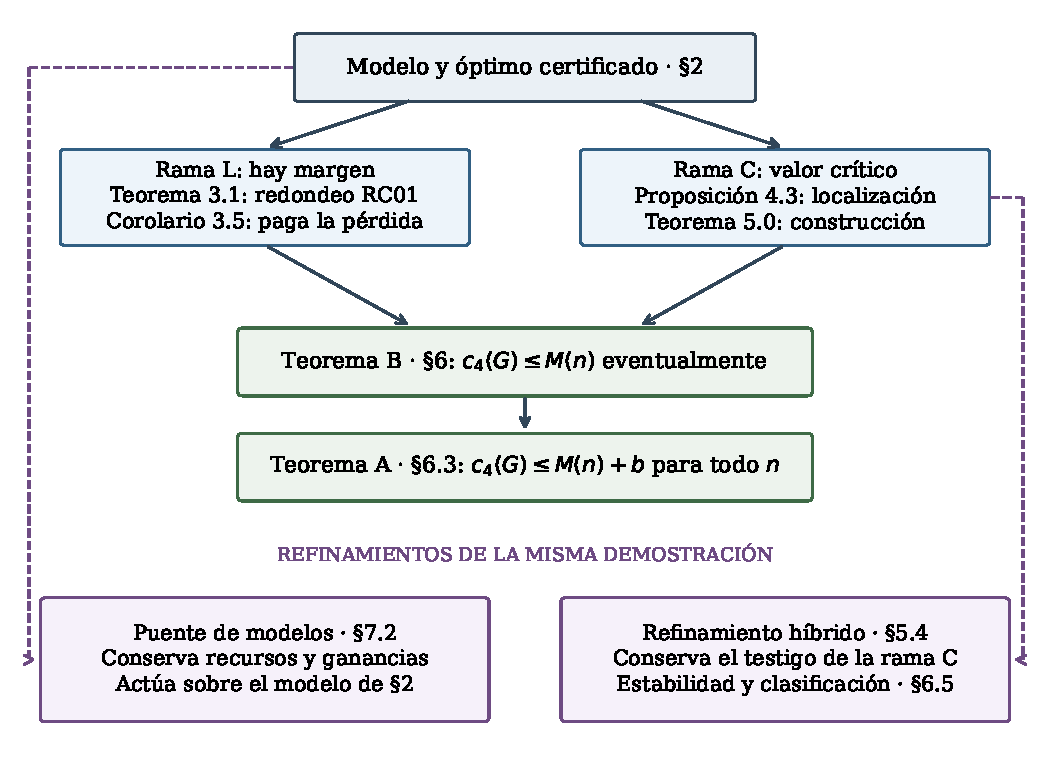
\includegraphics[width=.95\linewidth]{figures/fig2_prueba_y_variantes.pdf}
\caption{Mapa de la demostración. La rama L se desarrolla en el Teorema 3.1 y el Corolario 3.5; la rama C, en la Proposición 4.3 y el Lema 5.3. Las líneas continuas forman la prueba de los Teoremas A y B. Las discontinuas señalan refinamientos que no se necesitan para esas cotas: el puente de modelos de la Sección 7.2 y el testigo conservado de la Sección 5.4.}
\end{figure}

\subsubsection{1.3. Organización y uso de la cordalidad}\label{organizacion-y-uso-de-la-cordalidad}

\textbf{Observación 1.1.} La rama de redondeo vale para grafos arbitrarios. La rama crítica usa la cordalidad en tres puntos diferentes: la existencia y conservación de los pasos de copia de §4.1; la extracción de una clique y la ausencia de cuadrados inducidos en §5.1; y el orden de eliminación perfecto que orienta las aristas exteriores en §5.3. El orden de eliminación también certifica que los ejemplos que alcanzan la cota son cordales. Ninguna de esas propiedades se deduce sólo de las desigualdades numéricas del presupuesto.

La Sección 2 fija el modelo. La Sección 3 enuncia el redondeo y explica su uso; el Apéndice C desarrolla su prueba técnica. Las Secciones 4 y 5 establecen la localización y la construcción crítica. La Sección 6 ensambla la prueba y obtiene estabilidad, clasificación y valores exactos. La Sección 7 resume el alcance formal; el Apéndice A contiene las declaraciones y su correspondencia. La Sección 8 compara los mecanismos con {[}5,15{]}. El Apéndice B reúne herramientas complementarias.

En la numeración actual de la serie, el motor general de transferencia se reserva para Paper V. Las menciones a ese motor como «Paper IV» en versiones anteriores de {[}2--4{]} corresponden al plan antiguo, no a una dependencia adicional del presente resultado.

\subsection{2. Ganancia mixta, dualidad y particiones}\label{ganancia-mixta-dualidad-y-particiones}

Todos los grafos son finitos, simples y no dirigidos. Una clique se identifica con su conjunto de vértices; sus aristas son todas las parejas de vértices distintos de ese conjunto. Un grafo es cordal si no tiene un ciclo inducido de longitud al menos cuatro. Los subgrafos inducidos de un cordal son cordales.

\subsubsection{2.1. Por qué se redondea una ganancia}\label{por-que-se-redondea-una-ganancia}

Sea \(\mathcal K(G)\) la familia de las cliques de orden tres o cuatro. Un empaquetamiento mixto es una subfamilia \(\mathcal P\subseteq\mathcal K(G)\) de copias disjuntas por aristas. Definimos \[
g(K)=\binom{|K|}{2}-1,\qquad
g(\mathcal P)=\sum_{K\in\mathcal P}g(K).
\]

\Needspace{16\baselineskip}

{\def\LTcaptype{none} % do not increment counter
\begin{longtable}[c]{@{}lrrr@{}}
\toprule\noalign{}
Pieza & Aristas cubiertas & Piezas que sustituye & Ganancia \\
\midrule\noalign{}
\endhead
\bottomrule\noalign{}
\endlastfoot
\(K_2\) & 1 & 1 & 0 \\
\(K_3\) & 3 & 3 & 2 \\
\(K_4\) & 6 & 6 & 5 \\
\end{longtable}
}

\textbf{Tabla 1.} El coste se mide respecto de cubrir cada arista por separado.

\subsubsection{Lema 2.1}\label{lema-2.1}

Sea \(Q\) la partición obtenida al añadir a \(\mathcal P\) cada arista no cubierta como una pieza \(K_2\). Su número de piezas es exactamente \[
|Q|=e(G)-g(\mathcal P).
\tag{2.1}
\] \textbf{Demostración.} Las piezas de \(\mathcal P\) cubren \(\sum_K\binom{|K|}{2}\) aristas, porque no se solapan. Quedan \(e(G)-\sum_K\binom{|K|}{2}\) aristas individuales. Al sumar las \(|\mathcal P|\) piezas iniciales se obtiene (2.1). La cobertura es exacta por construcción.

\subsubsection{2.2. El óptimo fraccional y su certificado}\label{el-optimo-fraccional-y-su-certificado}

Un empaquetamiento fraccional asigna un peso \(x_K\ge0\) a cada copia real \(K\), con \[
\sum_{K:e\in E(K)}x_K\le1\qquad(e\in E(G)).
\tag{2.2}
\] Su valor es \(w(x)=\sum_K g(K)x_K\), y \(W^*(G)\) es el máximo de esos valores. El dual asigna precios \(y_e\ge0\) a las aristas. Para cada triángulo \(T\) y cada \(K_4\), denotado por \(Q\), exige respectivamente \[
\sum_{e\in E(T)}y_e\ge2,\qquad
\sum_{e\in E(Q)}y_e\ge5.
\tag{2.3}
\] La factibilidad primal contiene al vector cero. Cada coordenada primal está acotada por uno, puesto que toda copia contiene alguna arista. La dualidad finita proporciona óptimos primal y dual de igual valor. El modelo formal utiliza datos racionales y construye ambos óptimos: el valor \(w\) no entra como una suposición sin testigo. Paper I {[}2, Apéndice B{]} aporta el antecedente de dualidad empaquetamiento--cobertura; el desarrollo racional usado aquí prueba su versión mediante eliminación de Fourier--Motzkin.

De (2.2), sumando capacidades, resulta también \[
w(x)\le\frac56\sum_K |E(K)|x_K\le\frac56e(G).
\tag{2.4}
\] Esta estimación controla el coste de reducir multiplicativamente un empaquetamiento. No es por sí sola la cota extremal cordal.

\subsubsection{2.3. Relación con los funcionales anteriores}\label{relacion-con-los-funcionales-anteriores}

La extensión por cero de un empaquetamiento triangular da \[
W^*(G)\ge2\nu_3^*(G),\qquad
F_4(G)\le e(G)-2\nu_3^*(G).
\tag{2.5}
\] Paper II {[}3, Teorema 1.1{]} acota la segunda cantidad por \(\lfloor(2n+1)^2/24\rfloor\). Para \(n\) entero este piso coincide con \(M(n)\): el producto \(n(n+1)\) es congruente con 0 o 2 módulo 6 y sumar \(1/24\) no cruza un entero. Esto explica el objetivo de la serie. El paso desde ese valor fraccional a una partición sigue requiriendo las dos ramas posteriores.

\subsubsection{2.4. Notación de las dos ramas}\label{notacion-de-las-dos-ramas}

{\def\LTcaptype{none} % do not increment counter
\begin{longtable}[c]{@{}
  >{\raggedright\arraybackslash}p{(\linewidth - 2\tabcolsep) * \real{0.5000}}
  >{\raggedright\arraybackslash}p{(\linewidth - 2\tabcolsep) * \real{0.5000}}@{}}
\toprule\noalign{}
\begin{minipage}[b]{\linewidth}\raggedright
Símbolo
\end{minipage} & \begin{minipage}[b]{\linewidth}\raggedright
Significado
\end{minipage} \\
\midrule\noalign{}
\endhead
\bottomrule\noalign{}
\endlastfoot
\(M(n)\), \(B_n(p)\) & Objetivo entero y perfil completo-split \\
\(W^*(G)\), \(W(G)\) & Ganancias óptimas mixta fraccional y entera \\
\(g(\mathcal P)\) & Ganancia del empaquetamiento físico elegido \\
\(F_4=e-W^*\), \(\Delta=M-F_4\) & Coste fraccional y margen hasta el objetivo \\
\(W_S^*,F_S,\Delta_S\) & Las mismas cantidades para una familia de órdenes \(S\), sólo en §§1.1 y 8 \\
\(C,P,R\) & Núcleo del comparador, clique extraída y raíz regularizada \\
\(a,p,q\) & \(|P|,|R|,n-|R|\) \\
\(m,A\) & Aristas exteriores y enlaces ausentes respecto de \(R\) \\
\(f,\ell\) & Triángulos de la primera fase y bases fallidas de la segunda \\
\(d(G)\) & Distancia de edición normalizada a la familia completo-split \\
\end{longtable}
}

Los símbolos auxiliares del selector del Apéndice C se definen allí. En particular, \(\ell\) en §5 es un conteo de fallos y no una ganancia.

\subsection{3. Redondeo mixto y régimen con holgura}\label{redondeo-mixto-y-regimen-con-holgura}

Ésta es la rama L de la Figura 1. Su entrada es un empaquetamiento fraccional; su salida es uno físico con pérdida subcuadrática uniforme. El Corolario 3.5 explicará cuándo esa pérdida cabe dentro del margen disponible.

\subsubsection{Teorema 3.1}\label{teorema-3.1}

Para cada racional \(\xi>0\), existe \(N_\xi\) tal que, para todo grafo \(G\) de orden \(n\ge N_\xi\) y todo empaquetamiento fraccional mixto racional \(x\), existe un empaquetamiento mixto \(\mathcal P\) con \[
w(x)-g(\mathcal P)\le\xi n^2.
\tag{3.1}
\] No se exige cordalidad. El umbral se elige después de \(\xi\), pero antes de \(G\), \(n\) y \(x\).

Su alcance es una transferencia uniforme de la ganancia ponderada. Los teoremas de Haxell--Rödl y Yuster {[}6,7{]} proporcionan el contexto de transferencia fraccional a integral. Precisamos a continuación la entrada de Paper III y el adaptador de dos cuotas que conserva los pesos dos y cinco.

\textbf{Estructura de la demostración.} El lema de rango acotado de Paper III, reproducido como Lema 3.2 en el Apéndice C, redondea una familia con cargas a lo sumo uno y codegrado suficientemente pequeño. No distingue por sí solo las ganancias dos y cinco. El Lema 3.3 añade marcas y obtiene dos cuotas para un mismo emparejamiento; el Lema 3.4 agrupa parejas de triángulos y marca las copias de \(K_4\), de modo que la ganancia se recupera como cuatro veces la cuota total más la marcada.

Para aplicar ese selector a un grafo arbitrario, una partición regular y la limpieza de perfiles producen un sistema con cargas y codegrados controlados. La masa que se retira se carga una sola vez a sus recursos. Primero se fija \(\xi\), después los parámetros del selector y de regularidad, y sólo al final el umbral \(N_\xi\), independiente de la instancia. El caso de masa triangular pequeña se trata aparte. El Apéndice C conserva las estimaciones completas y la jerarquía de parámetros; su numeración 3.2--3.14 corresponde a la prueba de este teorema.

Por tanto, el Teorema 3.1 no se cita como una caja negra de Paper III. La entrada de ese paper es el nibble; la selección de dos cuotas, su realización mixta y el ensamblaje uniforme son los pasos de Paper IV. El contrato cerrado de (3.1) es todo lo que se usa a continuación.

\subsubsection{Corolario 3.5}\label{corolario-3.5}

Fijado un racional \(\eta>0\), todo grafo suficientemente grande con \(F_4(G)<n^2/6-\eta n^2\) admite una partición de orden a lo sumo cuatro con a lo sumo \(M(n)\) piezas.

\textbf{Demostración.} Se aplica el Teorema 3.1 a un óptimo racional con \(\xi=\eta/2\). El Lema 2.1 da \[
c_4(G)\le e(G)-g(\mathcal P)
\le F_4(G)+\frac\eta2n^2
<\frac{n^2}{6}-\frac\eta2n^2.
\] Para \(n\ge6\), la desigualdad \(\lfloor t\rfloor\ge t-1\) da \(M(n)\ge n(n+1)/6-1\ge n^2/6\). La conclusión se sigue aumentando el umbral si hace falta.

El argumento no necesita una cota lineal universal para \(W^*(G)-W(G)\). Sólo requiere que la pérdida sea menor que la holgura de la instancia.

\subsection{4. Localización del régimen crítico}\label{localizacion-del-regimen-critico}

Comenzamos la rama C de la Figura 1. La Proposición 4.3 localiza un comparador completo-split. La Sección 5 convierte esa información en una partición del grafo original.

Fijamos, como en el desarrollo formal, \[
\varepsilon_0=10^{-12},\qquad \eta_0=10^{-16}.
\tag{4.1}
\] El umbral cercano se ha reducido de \(10^{32}\) a \(4\cdot10^{12}\). Corresponde a la localización y al constructor cercano, no a toda la prueba: el redondeo de la Sección 3 puede imponer un umbral mayor. No se deduce de esa mejora un umbral global de \(4\cdot10^{12}\).

\subsubsection{4.1. Distancia a una familia fija}\label{distancia-a-una-familia-fija}

Para grafos sobre el mismo conjunto de vértices, sea \(d_E(G,H)=|E(G)\mathbin{\triangle}E(H)|\). Consideremos la familia de todos los completo-split etiquetados \(S_C=K_C\vee I_{V\setminus C}\), y definamos \[
d(G)=\frac1{n^2}\min_C d_E(G,S_C).
\] El mínimo se alcanza, porque la familia es finita. La desigualdad triangular implica \[
|d(G)-d(H)|\le\frac{d_E(G,H)}{n^2}.
\tag{4.2}
\] Una copia de un vértice modifica a lo sumo \(n-1\) aristas. Por tanto, el cambio de \(d\) en un paso es a lo sumo \(1/n\). Esta cota no exige que la distancia disminuya a lo largo de todo el camino.

Paper II {[}3{]} explica el mecanismo de copia de clases simpliciales y la terminación en un completo-split para el funcional triangular. El desarrollo mixto requiere sus propios transportes de valor y termina en un grafo de la misma familia. La cordalidad se conserva en las copias admisibles; la cota mixta no se deduce simplemente de cambiar el nombre del funcional triangular.

\Needspace{9\baselineskip}

\textbf{Lema 4.1 (camino mixto admisible).} Todo cordal \(G\) admite una sucesión finita \(G=G_0,\ldots,G_\ell\), sobre sus mismos vértices, tal que \(G_\ell\) es completo-split, cada \(G_i\) es cordal, cada paso copia un único vértice no adyacente y simplicial, y \[
F_4(G_i)\le F_4(G_{i+1}),\qquad
d_E(G_i,G_{i+1})\le n-1.
\tag{4.3}
\]

\textbf{Demostración.} Para dos vértices simpliciales no adyacentes \(u,v\), consideremos las dos copias opuestas \(G_{u\to v}\) y \(G_{v\to u}\). El transporte mixto de empaquetamientos da \[
W^*(G_{u\to v})+W^*(G_{v\to u})\le2W^*(G).
\tag{4.4}
\] Es la versión mixta del transporte de Paper II. Se transportan los dos empaquetamientos al grafo original y se toma su promedio con peso \(1/2\). Un enlace puede recibir carga de las piezas transportadas desde ambos extremos; el control previo es carga a lo sumo dos, no uno. El promedio restablece la capacidad uno y divide por dos también la suma de ganancias. La suma de los números de aristas de las dos copias es \(2e(G)\). Al restar (4.4) se obtiene \(2F_4(G)\le F_4(G_{u\to v})+F_4(G_{v\to u})\); al menos una dirección no disminuye \(F_4\).

Falta justificar que siempre existe un paso fuera del terminal y que los pasos no se repiten. Llamemos gemelos a dos vértices con el mismo vecindario abierto. Si todo par simplicial no adyacente fuera gemelo, Dirac proporciona, en el caso no completo, un par \(x,y\) con vecindario común \(C\), que es clique. El exterior de \(C\) es independiente: de contener una componente con una arista, la forma enraizada de Dirac daría en ella un vértice simplicial del grafo, cuyo vecindario tendría que ser \(C\), contradiciendo que tiene un vecino en esa componente. Cada vértice exterior es entonces simplicial y, por la condición sobre pares, tiene exactamente vecindario \(C\). Por tanto, el grafo es \(K_C\vee I_{V\setminus C}\). El caso completo ya es terminal. La contraposición da las dos clases distintas que requiere el paso.

Contemos ahora pares ordenados de gemelos distintos. Sean \(t\le s\) los tamaños de las dos clases, y copiemos un vértice de la menor hacia la mayor. Entre los vértices no copiados no se destruye ninguna igualdad de vecindarios: todos sufren la misma sustitución de la coordenada del vértice copiado. Se pierden a lo sumo \(2(t-1)\) pares que lo contenían y se ganan \(2s\), así que el incremento es al menos \(2(s-t+1)>0\). Si esta dirección no disminuye \(F_4\), aumenta lexicográficamente la pareja formada por \(F_4\) y ese conteo. Si disminuye \(F_4\), (4.4) obliga a que la dirección inversa lo aumente estrictamente; también aumenta la pareja. Hay sólo finitos grafos etiquetados sobre \(V\), de modo que el proceso termina.

Por último, al borrar el vértice que se va a copiar queda un inducido cordal. Reincorporarlo con el vecindario clique de la fuente añade un simplicial; cualquier ciclo que lo atraviese y tenga longitud al menos cuatro tiene la cuerda entre sus dos vecinos. Se conserva, pues, la cordalidad. Sólo cambian aristas incidentes al vértice copiado, a lo sumo \(n-1\). Esto prueba (4.3).

\Needspace{9\baselineskip}

\textbf{Lema 4.2 (cuenta dentro de la ventana).} Si \(X\) es cordal, \(n\ge4\cdot10^{12}\), \(F_4(X)\ge n^2/6-\eta_0n^2\) y \(d(X)<\varepsilon_0\), entonces \[
d(X)\le16D/n^2,\qquad D=\eta_0n^2+n/6+1/24.
\tag{4.5}
\]

\textbf{Demostración.} Aplique la construcción local del Teorema 5.0, cuya prueba no usa la Proposición 4.3. Su cuenta reforzada (5.15a) entrega una raíz clique \(R\) y una partición \(Q\) con \[
F_4(X)\le |Q|\le B_n(|R|)-\frac{117}{1825}m-\frac{12687}{20000}A.
\] La primera desigualdad se debe a que el óptimo fraccional domina la ganancia del empaquetamiento físico. Por (5.16), \(B_n(|R|)\le(2n+1)^2/24\). Al restar la cota inferior supuesta para \(F_4(X)\), resulta \[
\frac{117}{1825}m+\frac{12687}{20000}A\le D.
\] Como \(16(117/1825)>1\) y \(16(12687/20000)>10\), deducimos \(m+10A\le16D\). Puesto que \(R\) es clique, \(d_E(X,S_R)=m+A\le16D\), que prueba (4.5). La cuenta reforzada se obtiene dentro de la construcción \textbf{local bajo cercanía}; la localización global se demuestra a continuación usando este lema. Así no hay dependencia circular.

\subsubsection{4.2. Descenso desde el terminal}\label{descenso-desde-el-terminal}

El argumento de localización puede verse como una inducción hacia atrás. Supongamos que \(G_0,\ldots,G_\ell\) es un camino admisible y que \(G_\ell\) es completo-split. Su distancia es cero. La estimación local de cuentas asegura que, dentro de la ventana \(d(X)<\varepsilon_0\), los grafos del camino con el valor fraccional requerido satisfacen \[
d(X)\le\frac{16D}{n^2}<\varepsilon_0-\frac1n,\qquad
D=\eta_0n^2+\frac n6+\frac1{24}.
\tag{4.6}
\] La calibración verifica esta última desigualdad para \(n\ge4\cdot10^{12}\).

En concreto, la desigualdad a verificar es \[
\frac{16}{6n}+\frac1n+\frac{16}{24n^2}
<\varepsilon_0-16\eta_0.
\tag{4.6a}
\] El cambio tiene dos causas concretas. La cuenta (5.15a) reduce el factor de presupuesto de 20 a 16; además, el descenso admite la barrera interior máxima \(\varepsilon_0-1/n\), sin reservar por separado las mitades \(\varepsilon_0/2\) y \(\varepsilon_0/4\). La desigualdad (4.6a) se cumple en \(n=4\cdot10^{12}\) y su lado izquierdo decrece con \(n\). La desigualdad de contracción con esta barrera falla para \(n\le3.6\cdot10^{12}\) con los valores actuales de \(\varepsilon_0,\eta_0\) y el factor 16. Ese límite se refiere a esta calibración, no a todos los métodos posibles.

Si \(d(G_{i+1})<\varepsilon_0-1/n\), entonces (4.2) da \[
d(G_i)<\varepsilon_0.
\] Ahora se puede aplicar (4.6) a \(G_i\), lo que lo devuelve al intervalo \(d(G_i)<\varepsilon_0-1/n\). El paso se repite hasta el grafo original. Se usan una ventana exterior y una contracción interior; no se necesita escoger el primer índice que cruza un umbral.

Esta inducción no elimina la estimación de estabilidad local (4.6). Explica exactamente qué entrada permite sustituir la elección de primera entrada por un descenso. La monotonía del valor fraccional preserva las hipótesis numéricas, aunque la distancia oscile.

La misma propagación puede demostrarse eliminando el último paso y razonando por la longitud del camino. Son dos pruebas del lema de localización, no dos soluciones globales adicionales. Ninguna necesita escoger un índice mínimo.

El umbral cercano refleja la interacción de dos escalas: retirar \(u\) vértices del comparador cuesta a lo sumo \(un\), mientras que la cuenta cordal controla \(u(u+1)/2\) por el número de ediciones. Una versión parametrizada toma un presupuesto \(a^2/B\), con \(B\ge1\), una cota \(a\ge\alpha n\), con \(0<\alpha\le1\), y \(\eta\ge0\). Las condiciones \[
\varepsilon=\frac{\alpha^4}{8B^2},\qquad
1280B^2\eta\le\alpha^4,\qquad
n\ge\frac{1280B^2}{\alpha^4}
\] son suficientes para la contracción numérica del descenso. No se afirma que esa escala sea necesaria ni óptima. La calibración específica utilizada aquí aprovecha estimaciones más ajustadas y da el umbral cercano indicado en la Proposición 4.3.

\subsubsection{Proposición 4.3}\label{proposicion-4.3}

Sea \(G\) cordal, de orden \(n\ge4\cdot10^{12}\), y supongamos \[
F_4(G)\ge n^2/6-\eta_0n^2.
\] Existe un conjunto no vacío \(C\subseteq V(G)\) tal que \[
d_E(G,S_C)\le\varepsilon_0n^2,
\tag{4.7}
\] \[
(6|C|-2n-1)^2
\le24\left((\eta_0+6\varepsilon_0)n^2+\frac n6+\frac1{24}\right).
\tag{4.8}
\]

La localización anterior y la estimación del comparador producen (4.7)--(4.8). El conjunto \(C\) no se declara una clique de \(G\): lo es del comparador \(S_C\). La siguiente construcción obtiene una raíz que sí es clique del grafo original. Esta distinción evita trasladar una partición a través de un conjunto de ediciones que puede tener tamaño cuadrático.

\subsection{5. Raíz regularizada y cuentas físicas}\label{raiz-regularizada-y-cuentas-fisicas}

\subsubsection{Teorema 5.0. Constructor cercano bajo hipótesis locales}\label{teorema-5.0.-constructor-cercano-bajo-hipotesis-locales}

Sean \(\varepsilon_0=10^{-12}\), \(\eta_0=10^{-16}\) y \(G\) cordal de orden \(n\ge4\cdot10^{12}\). Supongamos \[
d(G)<\varepsilon_0,\qquad F_4(G)\ge n^2/6-\eta_0n^2.
\] Existen una clique \(R\) de \(G\), de tamaño \(p\) con \(|3p-n|\le n/50\), y una partición \(Q\) de orden a lo sumo cuatro tales que, si \(m=e(G-R)\) y \(A\) cuenta los enlaces ausentes entre \(R\) y su exterior, \[
|Q|\le B_n(p)-\frac m{20}-\frac A2,\qquad
B_n(p)=p(n-p)-\binom p2.
\tag{5.0}
\]

\textbf{Demostración y organización.} El Lema 5.1 extrae una clique real; la Proposición 5.2 la regulariza. Las dos fases de §§5.2--5.3 construyen sobre los mismos recursos un empaquetamiento cuya completación satisface la Tabla 2. El Lema 5.3 da (5.0). Para la ventana de tamaño, el Lema 5.1 da \(a\ge33n/100\). Las cuentas de regularización proporcionan \(99a\le100p\) y \(48(2p-(n-p))\le a\), interpretando la resta como truncada antes de pasar a la desigualdad racional. Junto con \(p+(n-p)=n\), estas relaciones implican \(3267n\le10000p\) y \(3539p\le1188n\), de donde \(|3p-n|\le n/50\). En particular, se conserva la ventana anterior \(n/4\le p\le n/2\). Ninguno de estos pasos usa la localización global de la Proposición 4.3. Así puede aplicarse el presente teorema en el Lema 4.2, y sólo después obtenerse esa localización. Los apartados siguientes prueban cada paso del contrato.

\subsubsection{5.1. Regularización sobre el grafo original}\label{regularizacion-sobre-el-grafo-original}

La construcción de esta sección es local: recibe un cordal \(G\) que ya satisface \(d(G)<\varepsilon_0\) y \(F_4(G)\ge n^2/6-\eta_0n^2\). Por eso puede utilizarse en el Lema 4.2 antes de concluir la localización global. Una vez demostrada la Proposición 4.3 se aplica al grafo original.

\Needspace{9\baselineskip}

\textbf{Lema 5.1 (extracción de una clique real).} Bajo esas hipótesis y \(n\ge4\cdot10^{12}\), existe una clique \(P\) de \(G\), de tamaño \(a\), tal que \[
\begin{gathered}
a\ge1024,\qquad |n-3a|\le a/64,\\
e(G-P)+\#\{\text{enlaces ausentes entre }P\text{ y }V\setminus P\}
\le a^2/65536.
\end{gathered}
\tag{5.1}
\]

\textbf{Demostración.} Sea \(C\) un núcleo del comparador más cercano y escribamos \(r=|C|\). La robustez fraccional por edición da \(|F_4(G)-F_4(S_C)|\le6d_E(G,S_C)\). Pongamos \(\delta_C=(\eta_0+6\varepsilon_0)n^2+n/6+1/24\); la hipótesis implica \(F_4(S_C)\ge(2n+1)^2/24-\delta_C\).

Expliquemos qué ocurre fuera del régimen split de muchos anfitriones. Escribamos \(a_0=\binom r2\), \(b_0=r(n-r)\). Los empaquetamientos fraccionales explícitos del comparador dan las cotas \[
F_4(S_C)\le
\begin{cases}
b_0-a_0,&b_0\ge2a_0,\\
(2b_0-a_0)/3,&a_0\le b_0\le2a_0,\\
(a_0+b_0)/6,&b_0\le a_0.
\end{cases}
\tag{5.1a}
\] Estas tres construcciones se aplican para \(r\ge4\) y exterior no vacío. La rama intermedia está acotada por \((4n+1)^2/120\), y la tercera por \(n(n-1)/12\). Para \(n\ge9\), ambas quedan estrictamente por debajo de \((2n+1)^2/24-n^2/40\). Como aquí \(\delta_C\le n^2/40\), ninguna satisface la hipótesis de cercanía fraccional. Si \(r<4\), basta la cota \(F_4(S_C)\le3n\); si el exterior es vacío, el empaquetamiento uniforme de \(K_4\) da \(F_4(S_C)\le n(n-1)/12\). Para \(n\ge100\), también se excluyen estos casos. Queda la primera rama: \(F_4(S_C)\le b_0-a_0=B_n(r)\). Completar el cuadrado da entonces \((6r-2n-1)^2\le24\delta_C\). Así se justifica la estimación sin extender indebidamente una identidad split a todos los tamaños de núcleo.

Tomemos ahora una clique máxima \(P\) del inducido cordal \(G[C]\), y pongamos \(u=r-a\). Un orden de eliminación perfecto acota sus aristas por \((a-1)r-\binom a2\). En consecuencia, faltan al menos \[
\binom r2-\left((a-1)r-\binom a2\right)
=\binom{u+1}{2}
\] pares dentro de \(C\). Todos ellos se cuentan entre las ediciones del comparador, por lo que \(u(u+1)/2\le\varepsilon_0n^2\). En particular, \(u\le3n/(2\cdot10^6)\). Al retirar esos \(u\) vértices del núcleo del comparador se modifican a lo sumo \(un\) pares adicionales. Por tanto, el defecto exterior y cruzado respecto de \(P\) suma a lo sumo \(\varepsilon_0n^2+un\).

Para ver la escala de la calibración, \(\delta_C\le(61/10)\varepsilon_0n^2\) sitúa \(r\) a distancia menor que \(3\cdot10^{-6}n\) de \(n/3\). Junto con la cota de \(u\), implica \(a\ge33n/100\) y \(|n-3a|\le a/64\). Además \[
\varepsilon_0n^2+un\le(10^{-12}+1.5\cdot10^{-6})n^2
\le\frac{(33n/100)^2}{65536}\le\frac{a^2}{65536}.
\] Son comparaciones racionales con las constantes fijadas en (4.1). El umbral de \(n\) da también \(a\ge1024\). Así se obtiene (5.1) sin tratar nunca \(C\) como clique de \(G\).

La raíz definitiva se define explícitamente. Se retiran de \(P\) los vértices cuya columna de enlaces ausentes tiene tamaño al menos \(|P|/4\), y se incorporan los vértices exteriores de grado exterior al menos \(7|P|/4\). Si esos conjuntos son \(X\) y \(Y\), respectivamente, \[
R=(P\setminus X)\cup Y.
\tag{5.2}
\] El presupuesto de defecto da \[
16384|X|\le |P|,\qquad 57344|Y|\le |P|.
\tag{5.3}
\] \Needspace{9\baselineskip}

\textbf{Proposición 5.2 (regularización).} La raíz \(R\) de (5.2) es clique. Si \(p=|R|\), \(q=n-p\), \(m=e(G-R)\), \(A\) es su defecto cruzado y \(D\) el máximo defecto de una columna, satisface las cotas de paleta y anchura de (5.7), y \[
\begin{gathered}
99a/100\le p\le101a/100,\quad q\ge p,\quad
44352q\ge87947a,\\
48(2p-q)_+\le a,\quad 3D\le a,\quad
400m<a^2,\quad2000(A+2m)\le11a^2.
\end{gathered}
\tag{5.4}
\]

\textbf{Demostración.} La suma de las columnas ausentes es parte del presupuesto (5.1), así que \((a/4)|X|\le a^2/65536\). La suma de los grados exteriores es el doble del número de aristas exteriores, y da \((7a/4)|Y|\le2a^2/65536\). Son las dos cotas de (5.3).

Toda clique exterior a \(P\) tiene a lo sumo \(a/128+1\) vértices: sus pares internos se cuentan en el mismo presupuesto. En un cordal, los vecinos comunes de dos vértices no adyacentes forman una clique, pues dos vecinos comunes no adyacentes completarían un cuadrado inducido. Si dos miembros de \(Y\) no fueran adyacentes, sus vecindarios exteriores tendrían intersección de tamaño al menos \(7a/2-129a/64=95a/64\), incompatible con la cota de clique exterior. Aquí se usó \(|V\setminus P|\le129a/64\), que se sigue de (5.1). Así, \(Y\) es clique. Si \(x\in P\) no es adyacente a un miembro de \(Y\), la misma propiedad acota los vecinos comunes exteriores por \(a/128+1\). El grado exterior del miembro de \(Y\) fuerza entonces al menos \(a/4\) ausencias en la columna de \(x\); por tanto \(x\in X\). Esto prueba que \(R\) es clique.

Para las cotas restantes se cuentan los recursos que cambian al retirar \(X\) e incorporar \(Y\). Si \(m_P,A_P\) son los defectos respecto de \(P\), se tiene \(m\le m_P+|X|n\) y \(A\le A_P+|Y|n\). Los grados y la anchura exteriores satisfacen \[
64d_{\max}(G-R)\le113a+64|X|,\qquad
128\omega(G-R)\le a+128+128|X|.
\] Las columnas retenidas parten de menos de \(a/4\) ausencias; las incorporadas se controlan con el mismo argumento de vecinos comunes. Sustituir (5.3), \(a\ge1024\) y \(127a\le64|V\setminus P|\le129a\) en estas cuentas da (5.4) y (5.7). Son las cotas que se consumen abajo: el defecto no se vuelve a elegir después de construir el empaquetamiento.

El objetivo de (5.2) no es minimizar una energía abstracta. Se separan los dos defectos que impedirían asignar anfitriones: columnas con demasiadas ausencias y vértices exteriores con demasiado grado residual. El resultado conserva cotas explícitas de tamaño, anchura exterior y disponibilidad de enlaces.

\subsubsection{5.2. De emparejamientos a triángulos}\label{de-emparejamientos-a-triangulos}

Un emparejamiento de bases \(uv\), junto con un vértice \(z\) adyacente a todos sus extremos, produce los triángulos \(zuv\). Son disjuntos por aristas: dentro del emparejamiento ningún extremo se repite, de modo que tampoco se repite un enlace a \(z\).

\begin{figure}[H]
\centering
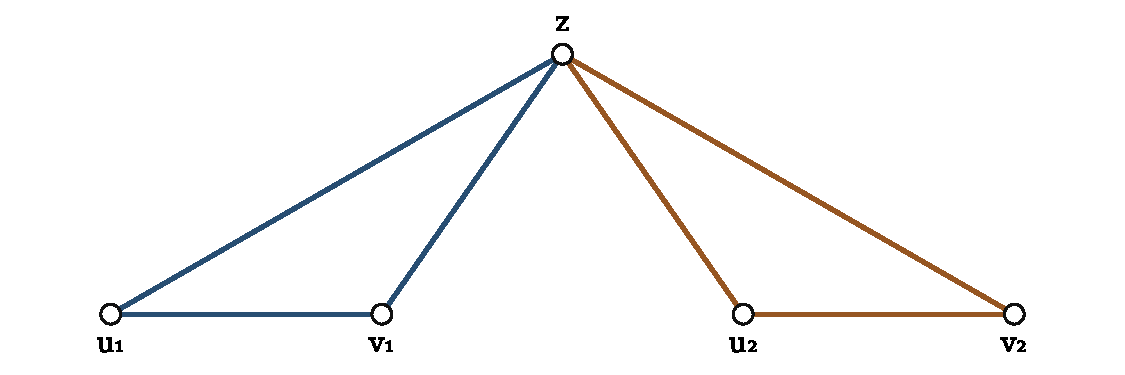
\includegraphics[width=.95\linewidth]{figures/fig3_anfitrion.pdf}
\caption{Dos bases disjuntas con un anfitrión común producen dos triángulos que comparten un vértice, pero ninguna arista. Esta es la unidad física utilizada en las asignaciones por clases de color.}
\end{figure}

Para varios anfitriones se exige, además, que sean distintos, que ningún anfitrión sea extremo de las bases y que las familias de bases sean disjuntas. Esas condiciones prueban la compatibilidad entre clases; no se suma la ganancia de construcciones cuya disjunción no haya sido verificada.

La primera fase aplica esta realización a aristas exteriores usando vértices de la raíz como anfitriones. Una coloración equilibrada y el orden de eliminación enraizado controlan cuántas bases pueden alojarse. La segunda fase factoriza las aristas de la raíz en matchings y les asigna candidatos exteriores. Las listas de candidatos excluyen tanto enlaces ausentes como recursos ya utilizados por la primera fase.

\subsubsection{5.3. Las tres cuentas que pagan la construcción}\label{las-tres-cuentas-que-pagan-la-construccion}

Para comparar la construcción real con el modelo completo-split, fijemos primero el tamaño de la raíz. Pongamos \(p=|R|\) y \(q=n-p\). Si todas las aristas entre la raíz y su exterior estuvieran presentes y no hubiera aristas exteriores, el coste de referencia sería \[
B_n(p)=p(n-p)-\binom p2.
\] En efecto, cubrir individualmente las aristas del completo-split costaría \(p(n-p)+\binom p2\) piezas. Cada una de las \(\binom p2\) bases internas se incorpora a un triángulo con un anfitrión exterior; ese triángulo sustituye tres aristas individuales por una pieza y ahorra dos. El coste resultante es, por tanto, \(p(n-p)+\binom p2-2\binom p2=B_n(p)\). Con esta referencia fijada \textbf{antes} de construir, introducimos las desviaciones reales. Sean \(m\) el número de aristas exteriores a \(R\), \(A\) el número de enlaces ausentes entre \(R\) y su exterior, \(f\) el número de triángulos de la primera fase y \(\ell\) el número de bases fallidas de la segunda. Si \(Q\) es la completación física, los lemas de construcción producen las tres relaciones siguientes.

\Needspace{16\baselineskip}

{\def\LTcaptype{none} % do not increment counter
\begin{longtable}[c]{@{}
  >{\raggedright\arraybackslash}p{(\linewidth - 4\tabcolsep) * \real{0.3333}}
  >{\raggedright\arraybackslash}p{(\linewidth - 4\tabcolsep) * \real{0.3333}}
  >{\raggedright\arraybackslash}p{(\linewidth - 4\tabcolsep) * \real{0.3333}}@{}}
\toprule\noalign{}
\begin{minipage}[b]{\linewidth}\raggedright
Cuenta
\end{minipage} & \begin{minipage}[b]{\linewidth}\raggedright
Identidad o desigualdad
\end{minipage} & \begin{minipage}[b]{\linewidth}\raggedright
Función
\end{minipage} \\
\midrule\noalign{}
\endhead
\bottomrule\noalign{}
\endlastfoot
Conteo de piezas & \(|Q|+A+2f=B_n(p)+m+2\ell\) & Expresa el coste real \\
Primera fase & \(1600m\le2920f+219A\) & Paga las aristas exteriores \\
Segunda fase & \(200\ell\le35A+8f\) & Acota las bases fallidas \\
\end{longtable}
}

\textbf{Tabla 2.} Todas las cantidades de pérdida proceden de familias finitas. El valor de referencia \(B_n(p)\) se fija antes de contar \(Q\).

La identidad del primer renglón se obtiene contando. Hay \(e(G)=\binom p2+pq+m-A\) aristas. La primera fase aporta \(f\) triángulos y la segunda \(\binom p2-\ell\). Como las familias son compatibles, el Lema 2.1 da \[
|Q|=\binom p2+pq+m-A-2\left(f+\binom p2-\ell\right)
=B_n(p)+m-A-2f+2\ell.
\tag{5.4a}
\] Reordenar esta igualdad da la primera cuenta. En particular, no se estima por separado el coste de dos construcciones que pudieran competir por las mismas aristas.

La compatibilidad tiene una verificación concreta. Si un triángulo de la primera fase usa una arista exterior \(uv\) y un anfitrión \(z\in R\), consume los enlaces \(zu,zv\). La segunda fase no puede asignar \(u\) ni \(v\) a una base que contenga \(z\). Ésta es la tercera condición de exclusión de {\ttfamily\small canonicalBad}; las otras dos exigen adyacencia a ambos extremos de la base. El lema {\ttfamily\small isSpokeCompa\discretionary{\hbox{\ensuremath{\hookrightarrow}}}{}{}tible\_\discretionary{\hbox{\ensuremath{\hookrightarrow}}}{}{}surviving\_\discretionary{\hbox{\ensuremath{\hookrightarrow}}}{}{}canonicalBad} demuestra que las asignaciones supervivientes no reutilizan esos enlaces. Finalmente, {\ttfamily\small RD09SpokeCom\discretionary{\hbox{\ensuremath{\hookrightarrow}}}{}{}patibility.\discretionary{\hbox{\ensuremath{\hookrightarrow}}}{}{}card\_\discretionary{\hbox{\ensuremath{\hookrightarrow}}}{}{}union\_\discretionary{\hbox{\ensuremath{\hookrightarrow}}}{}{}phases} da la suma exacta de los números de triángulos de las dos fases.

Demostremos las otras dos estimaciones. La primera cuenta cuántas aristas exteriores sobreviven a la asignación de anfitriones. La segunda cuenta cuántas bases internas pueden quedarse sin anfitrión después de esa elección. El orden importa: las listas de la segunda fase excluyen los enlaces que realmente utilizó la primera.

\textbf{Primera fase: selección de colores y pérdidas por incompatibilidad.} Escribamos \(H=G-R\), \(w=\omega(H)\) y \(c=\max\{p,d_{\max}(H)+1\}\), donde \(d_{\max}(H)\) es el grado máximo. Vizing proporciona una coloración propia con a lo sumo \(c\) colores. Entre las coloraciones sobre esa paleta, escogemos una que minimice la suma de cuadrados de los tamaños de sus clases. Si dos clases difirieran en al menos dos aristas, su unión contendría un camino alternante con una arista más del color mayor; intercambiar sus colores reduciría la suma de cuadrados. Por tanto, las clases difieren en tamaño a lo sumo uno, y cada una tiene a lo sumo \(t=\lceil m/c\rceil\) aristas.

Conservamos las \(p\) clases mayores. Si contienen \(m_0\) aristas en total, comparar su tamaño medio con el promedio de todas las clases da \[
m_0\ge\frac pc\,m.
\tag{5.5}
\] Tomamos un orden de eliminación perfecto que termina en \(R\) y orientamos cada arista exterior hacia su extremo posterior. Si \(u\to v\), los vecinos posteriores de \(u\) forman una clique, por lo que todo vecino de \(u\) en \(R\) también es vecino de \(v\). En consecuencia, los anfitriones inválidos para \(uv\) son exactamente los vértices de \(R\) no adyacentes a \(u\). Si \(a_u\) es su número, el vértice \(u\) contribuye a lo sumo \((w-1)a_u\) incidencias inválidas: tiene a lo sumo \(w-1\) vecinos posteriores exteriores. Sumando y usando \(\sum_{u\notin R}a_u=A\), obtenemos a lo sumo \((w-1)A\) incidencias inválidas.

Enumeramos las clases conservadas y la raíz cíclicamente. Entre los \(p\) desplazamientos, cada clase recibe cada anfitrión una vez. El promedio de aristas descartadas es, por tanto, a lo sumo \((w-1)A/p\). Algún desplazamiento conserva un número \(f\) de aristas que satisface \[
f\ge m_0-\frac{w-1}{p}A
\ge\frac pc\,m-\frac{w-1}{p}A.
\tag{5.6}
\] Cada arista conservada produce un triángulo. Dentro de una clase las bases forman un emparejamiento, y clases distintas tienen anfitriones distintos; de ahí la disjunción por aristas. Las cotas de paleta y anchura que entrega la raíz regularizada son \[
40c\le73p,\qquad 40(w-1)\le3p.
\tag{5.7}
\] Al sustituirlas en (5.6), resulta \(f\ge40m/73-3A/40\). Multiplicar por \(2920\) da precisamente \(1600m\le2920f+219A\), la primera estimación de la Tabla 2. El Apéndice A.2 identifica las declaraciones de selección y promedio.

\textbf{Segunda fase: uno o dos candidatos por factor.} Factorizamos \(K_p\) en matchings y, si hace falta, añadimos una clase vacía para trabajar con \(p\) factores. Puesto que \(q\ge p\), podemos dar un candidato a cada factor. Sea \(s=\max\{2p-q,0\}\). Elegimos \(s\) factores con un solo candidato y damos dos a cada factor restante. Los \(2p-s\) puestos disponibles se asignan inyectivamente a vértices exteriores: ningún candidato pertenece a dos factores.

Para \(x\in R\), sean \(a_x\) el número de enlaces ausentes y \(u_x\) el número de enlaces ya usados por la primera fase. Definamos \(d_x=a_x+u_x\). Tenemos \[
\sum_xa_x=A,\quad \sum_xu_x=2f,\quad
a_x\le D,\quad u_x\le2t,\quad
S:=\sum_xd_x=A+2f,
\tag{5.8}
\] donde \(D=\max_xa_x\). La última cota puntual procede de que el emparejamiento asignado a \(x\) tiene a lo sumo \(t\) bases. Para la base \(e=xy\), denotemos por \(b_e\) el número de candidatos inválidos: falta alguno de los enlaces \(xz,yz\), o ya fue usado. La unión de esas prohibiciones da \(b_e\le d_x+d_y\).

Las tres estimaciones de momentos se obtienen contando sobre las parejas no ordenadas de la raíz: \[
\begin{aligned}
\sum_e b_e&\le(p-1)S,\\
\sum_e b_e^2&\le(p-2)\sum_xd_x^2+S^2,\\
\sum_xd_x^2&\le(D+4t)A+4tf.
\end{aligned}
\tag{5.9}
\] La primera cuenta cada \(d_x\) en las \(p-1\) bases que contienen \(x\). Para la segunda se expande \(\sum_{x<y}(d_x+d_y)^2\): los cuadrados aparecen \(p-1\) veces, y los productos cruzados suman \(S^2-\sum_xd_x^2\). Para la tercera se usa, término a término, \[
(a_x+u_x)^2\le Da_x+4ta_x+2tu_x,
\] y se aplican las sumas de (5.8). Así, cada término de (5.9) procede de las incidencias reales ausentes u ocupadas.

Promediemos ahora sobre la elección uniforme de los \(s\) factores simples y sobre las inyecciones de candidatos. Una base con un candidato falla con probabilidad \(b_e/q\); con dos candidatos distintos falla con probabilidad \(b_e(b_e-1)/(q(q-1))\). Por ello su probabilidad total de fallo es \[
\frac{s}{p}\frac{b_e}{q}
+\left(1-\frac{s}{p}\right)\frac{b_e(b_e-1)}{q(q-1)}.
\tag{5.10}
\] Sumamos, usamos \((p-1)/p\le1\), \(b_e(b_e-1)\le b_e^2\) y (5.9). Alguna asignación tiene un número \(\ell\) de bases fallidas no mayor que el promedio, de modo que \[
\ell\le\frac{s}{q}(A+2f)
+\frac{(p-2)((D+4t)A+4tf)+(A+2f)^2}{q(q-1)}.
\tag{5.11}
\] Para cada base que no falla, escogemos uno de sus candidatos válidos. Las bases del mismo factor son disjuntas; las de factores distintos usan candidatos distintos. Además, la definición de candidato válido excluye todo enlace ya utilizado. Esto verifica simultáneamente la compatibilidad dentro de la segunda fase y con el empaquetamiento de la primera.

Falta evaluar (5.11) con las cotas que entrega la regularización. Denotemos por \(a=|P|\) el tamaño de la clique de referencia anterior a (5.2). El certificado cercano da \[
\begin{gathered}
a\ge1024,\quad \frac qa\ge\frac{87947}{44352},\quad
\frac pa\le\frac{101}{100},\quad \frac Da\le\frac13,\\
\frac ta\le\frac1{256},\quad \frac sa\le\frac1{48},\quad
\frac{A+2f}{a^2}\le\frac{11}{2000}.
\end{gathered}
\tag{5.12}
\] Estas cotas pertenecen al certificado de la raíz regularizada y a su primera fase. Por ejemplo, ese certificado da \(p\ge99a/100\), \(m<a^2/400\) y \(2000(A+2m)\le11a^2\). Como \(c\ge p\), el tamaño de cada clase satisface \(t\le m/p+1<a/396+1\le a/256\), donde la última comparación usa \(a\ge1024\). Además \(f\le m\), de modo que la cota de masa para \(A+2f\) se sigue de la de \(A+2m\). Se comprueba así que las cantidades de (5.12) son las de la construcción elegida, no parámetros ajustados después de contar los fallos. La cota de \(s\) necesita las estimaciones finas de (5.3), no sólo los extremos redondeados de \(p/a\) y \(q/a\). Si \(q_P=n-a\), entonces \(p=a-|X|+|Y|\), \(q=q_P+|X|-|Y|\), y \[
2p-q=2a-q_P-3|X|+3|Y|
\le a/64+3a/57344<a/48.
\tag{5.12a}
\] Tomar la parte positiva prueba \(s/a\le1/48\). Por su parte, el denominador conserva el término \(q-1\): \[
\frac{q(q-1)}{a^2}\ge
\left(\frac{87947}{44352}\right)^2
-\frac{87947}{44352\cdot1024}\ge\frac{393}{100}.
\tag{5.13}
\] El lado intermedio es aproximadamente \(3.93008\), mientras que la cota usada es \(3.93\). La diferencia es pequeña pero positiva; se conserva la comparación racional exacta, sin redondearla hacia arriba ni cambiar \(R_0\) en las cuentas siguientes. Para linealizar el numerador, usamos \((A+2f)^2\le(11/2000)a^2(A+2f)\) y \(p-2\le p\). Si escribimos \(Q_0=87947/44352\) y \(R_0=393/100\), los coeficientes de \(A\) y \(f\) quedan acotados, respectivamente, por \[
\begin{aligned}
\frac{1}{48Q_0}
+\frac{(101/100)(1/3+1/64)+11/2000}{R_0}
&\le\frac{11}{100},\\
\frac{1}{24Q_0}
+\frac{(101/100)/64+11/1000}{R_0}
&\le\frac{29}{1000}.
\end{aligned}
\tag{5.14}
\] Son comparaciones racionales directas. Obtenemos \(\ell\le11A/100+29f/1000\). Como \(A,f\ge0\), esta cota implica \(\ell\le7A/40+f/25\), que al multiplicar por \(200\) es la segunda estimación de la Tabla 2. Se han usado así las dos contribuciones, la de enlaces ausentes y la de enlaces ocupados, sobre una misma asignación física. El Apéndice A.2 identifica los lemas de momentos, promedio y calibración.

\subsubsection{Lema 5.3}\label{lema-5.3}

Si se conserva la estimación fuerte de (5.14) para la misma partición \(Q\), se obtiene \[
|Q|\le B_n(p)-\frac{117}{1825}m-\frac{12687}{20000}A
\le B_n(p)-\frac m{16}-\frac A2.
\tag{5.15a}
\] En particular, las tres cuentas de la Tabla 2 también implican la forma anterior \[
|Q|\le B_n(p)-\frac{19}{365}m-\frac{253}{500}A
\le B_n(p)-\frac m{20}-\frac A2.
\tag{5.15}
\]

\textbf{Demostración.} De la cuenta de segunda fase, \(\ell\le7A/40+f/25\). Al sustituir en la identidad de piezas, \[
|Q|\le B_n(p)+m-\frac{13}{20}A-\frac{48}{25}f.
\] La primera fase da \(f\ge40m/73-3A/40\). Su coeficiente en la desigualdad anterior es negativo; por ello se utiliza esta cota inferior. Los coeficientes resultantes son \[
1-\frac{48}{25}\frac{40}{73}=-\frac{19}{365},\qquad
-\frac{13}{20}+\frac{48}{25}\frac3{40}=-\frac{253}{500}.
\] Como \(m,A\ge0\), \(19/365\ge1/20\) y \(253/500\ge1/2\), se obtiene la segunda desigualdad.

Para (5.15a), se vuelve a la cota anterior a esa relajación, \(\ell\le11A/100+29f/1000\), sin modificar la asignación física. La identidad de piezas da \[
|Q|\le B_n(p)+m-\frac{39}{50}A-\frac{971}{500}f.
\] Al usar de nuevo \(f\ge40m/73-3A/40\), los coeficientes se convierten en \(-117/1825\) y \(-12687/20000\). Finalmente \(117/1825>1/16\) y \(12687/20000>1/2\). Esta reserva no requiere elegir otra raíz ni otro packing.

Por otra parte, \[
B_n(p)=\frac{(2n+1)^2}{24}-\frac{(6p-2n-1)^2}{24}.
\tag{5.16}
\] La forma entera de la misma identidad es (6.3): \(6B_n(p)+(n-3p)(n-3p+1)=n(n+1)\). Como el producto de dos enteros consecutivos es no negativo, \(6B_n(p)\le n(n+1)\). Ahora sí, la integralidad de \(B_n(p)\) da \(B_n(p)\le\lfloor n(n+1)/6\rfloor=M(n)\). No se ha identificado el piso con la función racional: la envolvente de (5.16) excede \(n(n+1)/6\) en \(1/24\), y ese término no debe borrarse.

\subsubsection{5.4. El testigo que conserva la prueba}\label{el-testigo-que-conserva-la-prueba}

La conclusión cercana entrega conjuntamente el comparador de (4.7)--(4.8), la raíz regularizada, un empaquetamiento en \(G\) y las cuentas de la Tabla 2. Por (5.15)--(5.16), su completación tiene coste a lo sumo \(M(n)\).

En particular, no se construye una partición barata en \(S_C\) para luego reparar todas sus diferencias con \(G\). Las ediciones sirven para localizar y calibrar la raíz. La partición se realiza directamente en \(G\), y las pérdidas se pagan mediante sus propias familias de aristas y triángulos.

\Needspace{9\baselineskip}

\textbf{Corolario 5.4 (geometría cuantitativa de la rama crítica).} Para todo cordal \(G\) de orden suficientemente grande, o bien \(F_4(G)<n^2/6-\eta_0n^2\), o bien existen una clique \(R\) del grafo original y un núcleo comparador \(C\) tales que \[
|3|R|-n|\le\frac n{50},\qquad
|3|C|-n|\le\frac n{10^4},\qquad
d_E(G,S_C)\le\varepsilon_0n^2,
\tag{5.17}
\] y, en la segunda rama, \[
\left|e(G)-\frac{5n^2}{18}\right|\le\frac{n^2}{10^4}.
\tag{5.18}
\] En (5.17) basta tomar \(n\ge4\cdot10^{12}\) además del umbral de la dicotomía. La clique real procede de las tres razones de regularización utilizadas en el Teorema 5.0. La cota de \(C\) se obtiene de (4.8) y la calibración. Si \(k=|C|=n/3+t\), entonces \(|t|\le n/30000\) y \[
e(S_C)=\binom k2+k(n-k)
=\frac{5n^2}{18}+\frac{2nt}{3}-\frac{t^2}{2}-\frac{k}{2}.
\] La última desigualdad se sigue al comparar esta cuenta con \(e(G)\) mediante (4.7). La constante \(5/9\) describe la densidad \emph{asintótica} relativa al grafo completo; no es una identidad de densidad para un orden finito. El corolario determina tamaños, no la unicidad de \(R\) o \(C\) como conjuntos.

\subsection{6. Ensamblaje y valor extremo}\label{ensamblaje-y-valor-extremo}

\subsubsection{Demostración del Teorema B: cota superior}\label{demostracion-del-teorema-b-cota-superior}

Sea \(N_{\mathrm{lej}}\) el umbral del Corolario 3.5 con \(\eta=\eta_0\), y tomemos \(N\ge\max\{N_{\mathrm{lej}},4\cdot10^{12},6\}\). Para un cordal \(G\) de orden \(n\ge N\), se construye un óptimo mixto certificado. Si \(F_4(G)<n^2/6-\eta_0n^2\), el Corolario 3.5 proporciona la partición. En caso contrario, las Secciones 4 y 5 producen el testigo cercano y la completación al objetivo. Los dos casos agotan los valores de \(F_4(G)\), y ambas salidas son particiones del mismo grafo original.

La elección del óptimo es interna al argumento. Tampoco queda pendiente elegir un parámetro de cercanía para cada grafo: \(\eta_0\), \(\varepsilon_0\) y todos los umbrales se fijan de antemano.

\subsubsection{6.1. Optimalidad irrestricta en completo-split}\label{optimalidad-irrestricta-en-completo-split}

Sea \(S=K_k\vee I_h\), con \(2\le k\le h\). Sus aristas se dividen en \(\binom k2\) aristas interiores y \(kh\) enlaces. El argumento de pesos de Paper III {[}4, Corolario 10.2a{]} asigna peso \(-1\) a las primeras y \(+1\) a los segundos.

Toda clique contiene a lo sumo un anfitrión. Si tiene uno y \(s\ge1\) vértices del núcleo, su peso es \[
s-\binom s2\le1.
\] Si está enteramente en el núcleo, su peso es negativo. Por tanto, cualquier partición \(\mathcal Q\), sin restricción en el orden de las cliques, satisface \[
|\mathcal Q|\ge kh-\binom k2.
\tag{6.1}
\]

Para alcanzar la cota, se factorizan las aristas de \(K_k\) en \(k-1\) matchings perfectos si \(k\) es par y en \(k\) matchings si \(k\) es impar. En el segundo caso basta factorizar \(K_{k+1}\) y retirar el vértice añadido. Como \(h\ge k\), cada clase recibe un anfitrión distinto. Se obtiene un triángulo por arista del núcleo, sin compartir enlaces. Tras completar los enlaces restantes con aristas individuales, el número total de piezas es \[
\binom k2+kh-2\binom k2=kh-\binom k2.
\] La igualdad obtenida expresa el número de piezas de esa partición. Junto con (6.1), prueba \[
\operatorname{cp}(S)=c_3(S)=c_4(S)=kh-\binom k2.
\tag{6.2}
\] El enunciado público auditado se expresa como una partición de orden a lo sumo cuatro y una cota inferior irrestricta; la construcción descrita utiliza triángulos y aristas.

\subsubsection{6.2. El máximo eventual}\label{el-maximo-eventual}

La elección del núcleo extremal se explica mediante una identidad. Para \(f(n,k)=k(n-k)-\binom k2\), con la resta interpretada en los enteros, \[
6f(n,k)+(n-3k)(n-3k+1)=n(n+1).
\tag{6.3}
\] El producto de dos enteros consecutivos es no negativo. Por eso \(f(n,k)\le M(n)\). Para alcanzar el piso, ese producto debe ser el resto de \(n(n+1)\) módulo seis, que vale cero o dos. Así, \(n-3k\) sólo puede pertenecer a \(\{-2,-1,0,1\}\). Al imponer su congruencia módulo tres se obtienen exactamente los tamaños \[
\begin{cases}
k=r,& n=3r,\\
k=r\text{ o }r+1,& n=3r+1,\\
k=r+1,& n=3r+2.
\end{cases}
\tag{6.4}
\] Dentro de la familia completo-split con \(2\le k\le n-k\), el tamaño óptimo es único salvo en la segunda fila, donde hay dos tamaños consecutivos. Ésta es la clasificación de núcleos de {\ttfamily\small SplitComplet\discretionary{\hbox{\ensuremath{\hookrightarrow}}}{}{}eRigidity.\discretionary{\hbox{\ensuremath{\hookrightarrow}}}{}{}optimal\_\discretionary{\hbox{\ensuremath{\hookrightarrow}}}{}{}cores}; no es, por sí sola, una clasificación de todos los cordales extremales.

Para \(n\ge6\), la elección \(k=\lceil n/3\rceil\) pertenece siempre a (6.4) y satisface \(2\le k\le h=n-k\). El grafo \(K_k\vee I_h\) es cordal: eliminamos primero los anfitriones, cuyos vecinos posteriores están en el núcleo completo, y después el núcleo. Es un orden de eliminación perfecto, formalizado en {\ttfamily\small PaperTheorem\discretionary{\hbox{\ensuremath{\hookrightarrow}}}{}{}s.\discretionary{\hbox{\ensuremath{\hookrightarrow}}}{}{}splitGraph\_\discretionary{\hbox{\ensuremath{\hookrightarrow}}}{}{}isChordal}. Por (6.2), este cordal alcanza \(M(n)\). Junto con la cota superior se obtiene el máximo del Teorema B.

\subsubsection{6.3. Todos los órdenes y optimalidad del término lineal}\label{todos-los-ordenes-y-optimalidad-del-termino-lineal}

\textbf{Demostración del Teorema A.} Fijemos un umbral global \(N\) del Teorema B y pongamos \(b=N^2\). Si \(n\ge N\), ya existe una partición con a lo sumo \(M(n)\) piezas. Si \(n<N\), cubrimos cada arista por separado. El número de piezas es \[
e(G)\le\binom n2\le N^2\le M(n)+b.
\] También cubre \(n=0\). Finalmente, \(M(n)\le n^2/6+n/6\); para \(n\ge1\), la constante \(C=b+1/6\) da la forma \(n^2/6+Cn\), y para \(n=0\) la partición es vacía. Esto demuestra la respuesta al problema sin excepciones de orden.

El testigo \(b=N^2\) depende del umbral \textbf{global}, no sólo del cercano \(4\cdot10^{12}\). Ahora puede elegirse de manera explícita. Definamos la torre de doses por \(T(0)=1\) y \(T(j+1)=2^{T(j)}\), y pongamos \[
h=4\cdot8^5\cdot2208^5\cdot4500^{105}\cdot(2\cdot10^{16})^{105}.
\] La cuenta del Apéndice C.3 permite tomar \[
N=T(h+7),\qquad b=N^2\le T(h+8).
\] En efecto, la rama lejana con \(\eta_0=10^{-16}\) requiere a lo sumo \(T(h+7)\), y este número también supera el umbral cercano. Para \(n<N\), la partición por aristas individuales tiene a lo sumo \(n^2\le N^2\) piezas. Finalmente, \(N\ge4\) permite aplicar la desigualdad entera \(N^2\le2^N=T(h+8)\).

Esta cota es explícita, pero no es práctica ni se afirma óptima. No demuestra que \(b=0\), ni sustituye la torre por un umbral polinomial. La evaluación incluye las constantes del selector marcado: no queda un umbral de redondeo sin especificar dentro de la expresión. La identidad con el término continuo sigue siendo \(M(n)=n^2/6+n/6-\vartheta_n\), con \(0\le\vartheta_n<1\).

\textbf{Optimalidad del coeficiente cuadrático.} El \(1/6\) de \(n^2/6\) no puede reducirse, aunque se permitan cliques de cualquier orden. En efecto, si una cota \(\operatorname{cp}(G)\le c n^2+C n\) valiera para todos los cordales de orden suficientemente grande, aplicaríamos esa cota al completo-split crítico de §6.2. Por (6.2) y la definición de \(M(n)\), obtendríamos \[
\frac{n^2+n}{6}-1\le M(n)\le cn^2+Cn.
\tag{6.5a}
\] Si \(c<1/6\), la diferencia \((1/6-c)n^2\) excede a \(|C|n+1\) para \(n\) grande, contradiciendo (6.5a). La declaración {\ttfamily\small SharpConstan\discretionary{\hbox{\ensuremath{\hookrightarrow}}}{}{}tOptimality.\discretionary{\hbox{\ensuremath{\hookrightarrow}}}{}{}erdos81\_\discretionary{\hbox{\ensuremath{\hookrightarrow}}}{}{}quadratic\_\discretionary{\hbox{\ensuremath{\hookrightarrow}}}{}{}constant\_\discretionary{\hbox{\ensuremath{\hookrightarrow}}}{}{}optimal} formaliza esta necesidad para \(c,C\in\mathbb Q\), y {\ttfamily\small erdos81\_\discretionary{\hbox{\ensuremath{\hookrightarrow}}}{}{}quadratic\_\discretionary{\hbox{\ensuremath{\hookrightarrow}}}{}{}constant\_\discretionary{\hbox{\ensuremath{\hookrightarrow}}}{}{}isLeast} combina la necesidad con el Teorema A. La extensión de la afirmación matemática a coeficientes reales se obtiene escogiendo racionales entre \(c\) y \(1/6\), y por encima de \(C\). Es distinta de la optimalidad del coeficiente \emph{lineal} que sigue; ninguna de las dos afirmaciones decide si \(b=0\).

Fijado el término cuadrático \(n^2/6\), el coeficiente \(1/6\) del término lineal también es óptimo. Dados \(c<1/6\) y una constante \(B_0\), para todos los órdenes suficientemente grandes el testigo completo-split satisface \[
\operatorname{cp}(G)=M(n)
\ge\frac{n^2}{6}+\frac n6-1
>\frac{n^2}{6}+cn+B_0.
\tag{6.5}
\] La última desigualdad se cumple en cuanto \((1/6-c)n>B_0+1\). La formalización {\ttfamily\small LinearCoeffi\discretionary{\hbox{\ensuremath{\hookrightarrow}}}{}{}cient.\discretionary{\hbox{\ensuremath{\hookrightarrow}}}{}{}linear\_\discretionary{\hbox{\ensuremath{\hookrightarrow}}}{}{}coefficient\_\discretionary{\hbox{\ensuremath{\hookrightarrow}}}{}{}optimal} da esta conclusión para parámetros racionales; la afirmación para parámetros reales se sigue escogiendo un racional entre \(c\) y \(1/6\) y otro mayor que \(B_0\). Así se distingue la optimalidad del término asintótico de la constante aditiva necesaria para los órdenes pequeños.

La restricción de orden también aclara el alcance del Teorema A: olvidar \(Q.\mathrm{OrderAtMost}\ 4\) entrega inmediatamente la forma \(\operatorname{cp}(G)\le M(n)+b\) del problema original. {\ttfamily\small LossBudget.\discretionary{\hbox{\ensuremath{\hookrightarrow}}}{}{}erdos81\_\discretionary{\hbox{\ensuremath{\hookrightarrow}}}{}{}cp\_\discretionary{\hbox{\ensuremath{\hookrightarrow}}}{}{}form\_\discretionary{\hbox{\ensuremath{\hookrightarrow}}}{}{}all\_\discretionary{\hbox{\ensuremath{\hookrightarrow}}}{}{}orders} y {\ttfamily\small erdos81\_\discretionary{\hbox{\ensuremath{\hookrightarrow}}}{}{}cp\_\discretionary{\hbox{\ensuremath{\hookrightarrow}}}{}{}form} registran ese paso para las dos cotas. La implicación inversa no es una regla válida para cotas arbitrarias: para \(n\ge2\), \(\operatorname{cp}(K_n)=1\), mientras que una pieza de orden a lo sumo cuatro cubre como máximo seis aristas, y por ello \(c_4(K_n)\ge\binom n2/6\). Esta comparación entre parámetros no demuestra una separación lógica entre los dos enunciados universales con el objetivo particular \(M(n)\).

\subsubsection{6.4. El exceso de una partición completo-split}\label{el-exceso-de-una-particion-completo-split}

Mantengamos el régimen \(2\le k\le h\) de la Sección 6.1. Su argumento de pesos admite una lectura pieza por pieza. Para una clique \(C\) de \(K_k\vee I_h\), definamos \[
d(C)=1+e_{\rm int}(C)-e_{\rm cruz}(C),
\] donde se cuentan por separado las aristas internas del núcleo y las que unen núcleo y anfitrión. Entonces, para toda partición \(\mathcal Q\), sin restricción de orden, \[
|\mathcal Q|-\left(kh-\binom k2\right)
=\sum_{C\in\mathcal Q}d(C).
\tag{6.6}
\] \textbf{Demostración.} Las aristas internas suman \(\binom k2\) sobre las piezas y las cruzadas suman \(kh\), porque la cobertura es exacta. Sumando la definición se obtiene (6.6). Si \(C\) tiene un anfitrión y \(s\ge1\) vértices del núcleo, \[
d(C)=1+\binom s2-s=\frac{(s-1)(s-2)}2\ge0;
\] si no tiene anfitrión, \(d(C)=1+\binom{|C|}2>0\). No hay piezas contenidas sólo en los anfitriones: éstos forman un conjunto independiente y las piezas tienen al menos dos vértices. Los casos anteriores son, por tanto, exhaustivos. El defecto es cero exactamente en las aristas núcleo--anfitrión y los triángulos con dos vértices de núcleo y un anfitrión. Una partición óptima sólo utiliza esas piezas. Más generalmente, una partición con exceso a lo sumo \(t\) tiene a lo sumo \(t\) piezas de defecto positivo, pues cada una aporta al menos una unidad a (6.6). No se afirma unicidad de la partición óptima: puede haber distintas asignaciones de los mismos tipos de pieza.

\subsubsection{6.5. Estabilidad integral y clasificación de los extremizadores}\label{estabilidad-integral-y-clasificacion-de-los-extremizadores}

El argumento de la cota superior conserva la cuenta cercana reforzada (5.15a), aunque el Teorema B sólo necesita (5.15). Un grafo cuyo número óptimo de piezas está cerca de \(M(n)\) no puede pertenecer a la rama lejana, donde el redondeo produce una partición bastante por debajo de ese objetivo. La cuenta conservada convierte entonces un déficit integral pequeño en cotas para las aristas exteriores y los enlaces ausentes. Una vez elegida la raíz, una identidad por piezas controla toda partición próxima al mismo objetivo; no se elige de nuevo la raíz para cada partición.

\Needspace{9\baselineskip}

\textbf{Teorema 6.1 (estabilidad integral).} Existe \(\gamma>0\) y un umbral \(N_{\rm est}\) tales que, si \(n\ge N_{\rm est}\), \(G\) es cordal, \(0\le\delta\le\gamma n^2\) y toda partición de orden a lo sumo cuatro tiene al menos \(M(n)-\delta\) piezas, entonces existe una clique \(R\) de \(G\) para la cual \[
\bigl(M(n)-B_n(|R|)\bigr)+\frac m{16}+\frac A2\le\delta,
\qquad
d_E(G,S_R)=m+A\le16\delta.
\tag{6.7}
\] Aquí \(m=e(G-R)\) y \(A\) es el número de enlaces ausentes entre \(R\) y \(V(G)\setminus R\).

Expliquemos la prueba. Se toma \(\gamma=\eta_0/4\) y se aplica la dicotomía. En la rama lejana, RC01 conserva al menos \(\eta_0n^2/2\) de margen y produce una partición con \[
|Q|<\frac{n^2}{6}-\frac{\eta_0}{2}n^2
\le M(n)-\frac{\eta_0}{2}n^2.
\] Esto contradice \(|Q|\ge M(n)-\delta\), porque \(\delta\le\eta_0n^2/4\). Por tanto, sólo puede ocurrir la rama cercana. Allí la cuenta fuerte (5.15a), conservada para el mismo testigo físico, da \[
M(n)-\delta\le |Q|
\le B_n(|R|)-\frac m{16}-\frac A2,
\] de donde sale la primera desigualdad de (6.7). Como \(B_n(|R|)\le M(n)\) y \(A\ge0\), \[
m+A\le16\left(\frac m{16}+\frac A2\right)\le16\delta.
\] Finalmente, que \(R\) sea clique identifica exactamente las ediciones necesarias para transformar \(G\) en \(S_R\): se eliminan las \(m\) aristas exteriores y se añaden los \(A\) enlaces ausentes. Esto prueba la igualdad de (6.7).

La misma raíz controla no sólo al grafo, sino también a sus particiones cercanas al máximo. Para cualquier partición \(Q\), incluso si admite cliques de más de cuatro vértices, escribamos \(a_K=|K\cap R|\) y \(b_K=|K\setminus R|\) para cada pieza \(K\). Definimos su defecto respecto de \(R\) por \[
d_R(K)=1+\binom{a_K}{2}+3\binom{b_K}{2}-a_Kb_K
=\frac{(a_K-b_K)(a_K-b_K-1)}2+(b_K-1)^2.
\tag{6.7a}
\] El primer término de la derecha es no negativo para todo entero \(a_K-b_K\). Por tanto \(d_R(K)=0\) exactamente para las aristas raíz--exterior y los triángulos con dos vértices en la raíz y uno fuera.

\Needspace{9\baselineskip}

\textbf{Corolario 6.1a (estabilidad de las particiones).} Bajo las hipótesis del Teorema 6.1, la raíz \(R\) puede elegirse de forma que, para toda partición \(Q\) en cliques de \(G\), sin restricción en el orden de sus piezas, si \(|Q|\le M(n)+\tau\) con \(\tau\ge0\), entonces \(Q\) tiene a lo sumo \(\tau+48\delta\) piezas distintas de esas dos formas canónicas.

\textbf{Demostración.} La cobertura exacta de las aristas internas de \(R\), las exteriores y las cruzadas da, respectivamente, \(\binom{|R|}{2}\), \(m\) y \(|R|(n-|R|)-A\). Al sumar (6.7a) sobre las piezas resulta la identidad \[
\sum_{K\in Q}d_R(K)=|Q|-B_n(|R|)+A+3m.
\tag{6.7b}
\] Cada pieza no canónica contribuye al menos uno. Si \(r=M(n)-B_n(|R|)\), la hipótesis sobre \(Q\) deja a lo sumo \(\tau+r+A+3m\) de defecto. La reserva de (6.7) implica \(r+A+3m\le48\delta\). La raíz procede del testigo del Teorema 6.1 y no depende de \(Q\).

\Needspace{9\baselineskip}

\textbf{Corolario 6.2 (clasificación eventual).} Los cordales extremales de orden suficientemente grande son exactamente los completo-split con los tamaños de núcleo de (6.4).

\textbf{Demostración.} Al poner \(\delta=0\), (6.7) fuerza \(m=A=0\), luego \(G=S_R\). La identidad aritmética \[
6B_n(k)+(n-3k)(n-3k+1)=n(n+1)
\tag{6.8}
\] clasifica entonces los tamaños que alcanzan \(M(n)\). En consecuencia, para \(n\) suficientemente grande, \[
\operatorname{cp}(G)=M(n)
\quad\Longleftrightarrow\quad
c_4(G)=M(n)
\quad\Longleftrightarrow\quad
G\text{ es completo-split con núcleo óptimo},
\tag{6.9}
\] donde el tamaño del núcleo es \(r\) si \(n=3r\), \(r\) o \(r+1\) si \(n=3r+1\), y \(r+1\) si \(n=3r+2\). La equivalencia usa la cota inferior irrestricta de la Sección 6.1; por eso clasifica simultáneamente los extremizadores para \(\operatorname{cp}\) y para \(c_4\).

\Needspace{14\baselineskip}

\subsubsection{6.6. Coincidencia de los óptimos mixtos en completo-split}\label{coincidencia-de-los-optimos-mixtos-en-completo-split}

\Needspace{9\baselineskip}

\textbf{Proposición 6.3 (gap mixto nulo en completo-split).} Sea \(S=K_k\vee I_h\), con \(2\le k\le h\), y sea \(W(S)\) la máxima ganancia de un empaquetamiento mixto físico. Entonces \[
W^*(S)=W(S)=2\binom k2.
\tag{6.10}
\] Para justificar la cota fraccional, sea \(j(K)\) el número de aristas del núcleo que contiene una pieza mixta \(K\). Una clique de \(S\) tiene a lo sumo un anfitrión. Un triángulo con anfitrión tiene \(j(K)=1\) y ganancia dos; un \(K_4\) con anfitrión tiene \(j(K)=3\) y ganancia cinco. Las piezas enteramente en el núcleo también satisfacen \(g(K)\le2j(K)\). Así, para todo empaquetamiento fraccional factible \(x\), \[
\begin{aligned}
w(x)&\le2\sum_K j(K)x_K\\
&=2\sum_{e\in E(K_k)}\sum_{K:e\in E(K)}x_K
\le2\binom k2.
\end{aligned}
\tag{6.11}
\] La última desigualdad usa la capacidad uno de cada arista del núcleo. La construcción de la Sección 6.1 contiene un triángulo por base interna y alcanza esa ganancia. Como todo empaquetamiento entero define uno fraccional, quedan probadas las dos igualdades de (6.10). El resultado formal es {\ttfamily\small SplitMixedGa\discretionary{\hbox{\ensuremath{\hookrightarrow}}}{}{}p.\discretionary{\hbox{\ensuremath{\hookrightarrow}}}{}{}mixed\_\discretionary{\hbox{\ensuremath{\hookrightarrow}}}{}{}gap\_\discretionary{\hbox{\ensuremath{\hookrightarrow}}}{}{}zero}, junto con la construcción acotada de {\ttfamily\small SplitComplet\discretionary{\hbox{\ensuremath{\hookrightarrow}}}{}{}eSharpValue}.

La conclusión es una igualdad de valores óptimos en esta familia y bajo \(2\le k\le h\). No afirma que todos los vértices del politopo fraccional sean enteros, ni extiende el gap cero a cualquier grafo split.

\subsubsection{6.7. Reserva exacta por desplazamiento del núcleo}\label{reserva-exacta-por-desplazamiento-del-nucleo}

La identidad (6.3) permite conservar también el piso. Para enteros \(0\le k\le n\) con \(\binom k2\le k(n-k)\), definamos \[
d_{n,k}=\begin{cases}n-3k,&3k\le n,\\3k-n-1,&3k>n.\end{cases}
\] Entonces la reserva del perfil completo-split es exactamente \[
M(n)=B_n(k)+M(d_{n,k}).
\tag{6.12}
\] En efecto, en las dos ramas \(d_{n,k}(d_{n,k}+1)=(n-3k)(n-3k+1)\). Al sustituirlo en (6.3), dividir por seis y tomar pisos, el entero \(B_n(k)\) sale del piso y se obtiene (6.12). La hipótesis sobre \(\binom k2\) deja \(B_n(k)\) no negativo, tal como lo representa la declaración formal en naturales.

Esta forma identifica el margen disponible sin reemplazar \(M\) por su envolvente racional. En particular, la reserva es cero exactamente cuando \(d_{n,k}\le1\), lo que recupera los núcleos óptimos de (6.4). No proporciona por sí sola una partición de un cordal arbitrario: cuantifica el presupuesto del perfil con el que se compara la construcción.

\subsection{7. Formalización, código y reproducibilidad}\label{formalizacion-codigo-y-reproducibilidad}

El suplemento Lean identificado de esta versión usa Lean y Mathlib v4.28.0. Las declaraciones finales no reciben como argumentos el redondeo, la existencia del óptimo ni el constructor cercano: los invocan como teoremas demostrados en sus dependencias. Los axiomas fundacionales permitidos se distinguen de cualquier hipótesis matemática adicional.

El alcance formal difiere del documentado por {[}5{]} en el commit citado. Su archivo \nolinkurl{lean/FORMALIZATION_STATUS.md} declara una verificación condicionada a {\ttfamily\small ExternalInpu\discretionary{\hbox{\ensuremath{\hookrightarrow}}}{}{}ts.\discretionary{\hbox{\ensuremath{\hookrightarrow}}}{}{}Inputs}: Vizing, Häggkvist--Janssen y una transferencia de empaquetamiento que incluye certificados de optimalidad racional. Esas entradas son parámetros explícitos, no axiomas ocultos. Aquí se descargan las entradas empleadas por nuestra cadena, incluido Vizing; no se utiliza Häggkvist--Janssen. La comparación concierne a lo comprobado por cada desarrollo Lean: no afirma que la demostración matemática de {[}5{]} quede condicionada a conjeturas.

Los identificadores formales se imprimen con letra monoespaciada. Una flecha de continuación en un salto de línea es una marca tipográfica, no parte del identificador; las fuentes Markdown y Lean conservan su escritura literal.

La configuración declara Mathlib como paquete de terceros y una selección de los módulos {\ttfamily\small Nibble} de Paper III como dependencia local de la serie. {\ttfamily\small ConeAudit} recorre los tipos y términos de prueba de las declaraciones seleccionadas y comprueba que sus dependencias transitivas no contienen nombres bajo la raíz {\ttfamily\small Erdos81}, utilizada por {[}5{]}. La ausencia de esos nombres es un resultado reproducible del auditor, no una lectura de la lista de importaciones. Su alcance es preciso: certifica ese veto en el corte examinado; no detectaría por sí solo código trasladado y renombrado, ni determina la procedencia histórica de cada argumento. La atribución de fuentes se documenta por separado. La misma prueba de namespace no permite emitir un veredicto sobre {[}15{]}.

La auditoría adicional {\ttfamily\small PublicationI\discretionary{\hbox{\ensuremath{\hookrightarrow}}}{}{}ncrementAudi\discretionary{\hbox{\ensuremath{\hookrightarrow}}}{}{}t} incluye los enunciados públicos de {\ttfamily\small DefectSharpP\discretionary{\hbox{\ensuremath{\hookrightarrow}}}{}{}ublication}: en particular, el Teorema C, su testigo inferior y su máximo eventual. El build local combinado también ejecutó esa auditoría, con veto de los módulos históricos sustituidos. La interfaz {\ttfamily\small PaperIV.\discretionary{\hbox{\ensuremath{\hookrightarrow}}}{}{}Editorial.\discretionary{\hbox{\ensuremath{\hookrightarrow}}}{}{}ConstructorB\discretionary{\hbox{\ensuremath{\hookrightarrow}}}{}{}udget} de E.1 forma parte del mismo corte y pasó su auditoría separada, conservando la misma partición en sus dos conclusiones. La correspondencia entre fuentes y manuscrito fue examinada en la auditoría interna del autor; requiere aún examen adversarial independiente.

{\def\LTcaptype{none} % do not increment counter
\begin{longtable}[c]{@{}
  >{\raggedright\arraybackslash}p{(\linewidth - 2\tabcolsep) * \real{0.5000}}
  >{\raggedright\arraybackslash}p{(\linewidth - 2\tabcolsep) * \real{0.5000}}@{}}
\toprule\noalign{}
\begin{minipage}[b]{\linewidth}\raggedright
Resultado del texto
\end{minipage} & \begin{minipage}[b]{\linewidth}\raggedright
Módulo de referencia
\end{minipage} \\
\midrule\noalign{}
\endhead
\bottomrule\noalign{}
\endlastfoot
\textbf{Entradas y construcción} & \\
Óptimo racional alcanzado & {\ttfamily\small PaperI.\discretionary{\hbox{\ensuremath{\hookrightarrow}}}{}{}FiniteLPDual\discretionary{\hbox{\ensuremath{\hookrightarrow}}}{}{}ity}, {\ttfamily\small CertifiedOpt\discretionary{\hbox{\ensuremath{\hookrightarrow}}}{}{}imumExistenc\discretionary{\hbox{\ensuremath{\hookrightarrow}}}{}{}e} \\
Redondeo mixto uniforme, Teorema 3.1 & {\ttfamily\small RC01Final}, {\ttfamily\small MixedRoundin\discretionary{\hbox{\ensuremath{\hookrightarrow}}}{}{}gAdapter}; infraestructura \nolinkurl{Nibble.*} de Paper III \\
Corolario 3.5, régimen lejano para todos los grafos & {\ttfamily\small FarRegimeAll\discretionary{\hbox{\ensuremath{\hookrightarrow}}}{}{}Graphs.\discretionary{\hbox{\ensuremath{\hookrightarrow}}}{}{}farRegime\_\discretionary{\hbox{\ensuremath{\hookrightarrow}}}{}{}cliquePartit\discretionary{\hbox{\ensuremath{\hookrightarrow}}}{}{}ion\_\discretionary{\hbox{\ensuremath{\hookrightarrow}}}{}{}allGraphs}; versión explícita en {\ttfamily\small E17.\discretionary{\hbox{\ensuremath{\hookrightarrow}}}{}{}ExplicitFarA\discretionary{\hbox{\ensuremath{\hookrightarrow}}}{}{}ssembly} \\
Limpieza completa mejorada y umbral explícito & {\ttfamily\small E17.\discretionary{\hbox{\ensuremath{\hookrightarrow}}}{}{}Cleanup}, {\ttfamily\small E17.\discretionary{\hbox{\ensuremath{\hookrightarrow}}}{}{}FarBudget}, {\ttfamily\small E17.\discretionary{\hbox{\ensuremath{\hookrightarrow}}}{}{}ExplicitFarR\discretionary{\hbox{\ensuremath{\hookrightarrow}}}{}{}ounding}, {\ttfamily\small E17.\discretionary{\hbox{\ensuremath{\hookrightarrow}}}{}{}ExplicitFarA\discretionary{\hbox{\ensuremath{\hookrightarrow}}}{}{}ssembly}; constantes de {\ttfamily\small E18} y {\ttfamily\small E19} \\
Selección fraccional por nibble, Paper III & {\ttfamily\small Nibble.\discretionary{\hbox{\ensuremath{\hookrightarrow}}}{}{}FracNibbleLE}, {\ttfamily\small Nibble.\discretionary{\hbox{\ensuremath{\hookrightarrow}}}{}{}FracNibbleRe\discretionary{\hbox{\ensuremath{\hookrightarrow}}}{}{}paired}; adaptadores {\ttfamily\small PaperIIISlac\discretionary{\hbox{\ensuremath{\hookrightarrow}}}{}{}kNibbleAdapt\discretionary{\hbox{\ensuremath{\hookrightarrow}}}{}{}er}, {\ttfamily\small PaperIIINibb\discretionary{\hbox{\ensuremath{\hookrightarrow}}}{}{}leAdapter} \\
Localización, raíz y ventana crítica & {\ttfamily\small NearH1Locali\discretionary{\hbox{\ensuremath{\hookrightarrow}}}{}{}zation}, {\ttfamily\small NearRootWind\discretionary{\hbox{\ensuremath{\hookrightarrow}}}{}{}ow}, {\ttfamily\small RootRegulari\discretionary{\hbox{\ensuremath{\hookrightarrow}}}{}{}zationBridge} \\
Dicotomía e interfaz absorbible & {\ttfamily\small HybridDichot\discretionary{\hbox{\ensuremath{\hookrightarrow}}}{}{}omy}, {\ttfamily\small SeparationAb\discretionary{\hbox{\ensuremath{\hookrightarrow}}}{}{}sorptionRout\discretionary{\hbox{\ensuremath{\hookrightarrow}}}{}{}e} \\
Cuentas y partición cercana & {\ttfamily\small RD09Physical\discretionary{\hbox{\ensuremath{\hookrightarrow}}}{}{}Ledger}, {\ttfamily\small NearH1FinalA\discretionary{\hbox{\ensuremath{\hookrightarrow}}}{}{}ssembly}, {\ttfamily\small NearH1LocalC\discretionary{\hbox{\ensuremath{\hookrightarrow}}}{}{}onstructor} \\
\textbf{Conclusiones extremales} & \\
Cota aguda y máximo eventual & {\ttfamily\small Erdos81Uncon\discretionary{\hbox{\ensuremath{\hookrightarrow}}}{}{}ditional}, {\ttfamily\small PaperTheorem\discretionary{\hbox{\ensuremath{\hookrightarrow}}}{}{}s} \\
Cotas para todos los órdenes & {\ttfamily\small Erdos81AllOr\discretionary{\hbox{\ensuremath{\hookrightarrow}}}{}{}ders}; cota explícita en {\ttfamily\small ExplicitThre\discretionary{\hbox{\ensuremath{\hookrightarrow}}}{}{}shold} \\
Defecto enraizado fijo y máximo, Teorema C & {\ttfamily\small DefectSharpP\discretionary{\hbox{\ensuremath{\hookrightarrow}}}{}{}ublication}; constructor {\ttfamily\small A4S1.\discretionary{\hbox{\ensuremath{\hookrightarrow}}}{}{}IndepAllMain} \\
Necesidad de orden cuatro, Proposición D.2 & {\ttfamily\small DefectSharpP\discretionary{\hbox{\ensuremath{\hookrightarrow}}}{}{}ublication.\discretionary{\hbox{\ensuremath{\hookrightarrow}}}{}{}order\_\discretionary{\hbox{\ensuremath{\hookrightarrow}}}{}{}three\_\discretionary{\hbox{\ensuremath{\hookrightarrow}}}{}{}insufficient}, {\ttfamily\small E11K10} \\
Presupuesto general y paso a \(\operatorname{cp}\) & {\ttfamily\small LossBudget}, {\ttfamily\small SplitMixedGa\discretionary{\hbox{\ensuremath{\hookrightarrow}}}{}{}p} \\
Estabilidad del grafo, estabilidad de las particiones y clasificación & {\ttfamily\small IntegralStab\discretionary{\hbox{\ensuremath{\hookrightarrow}}}{}{}ility}, {\ttfamily\small RootPartitio\discretionary{\hbox{\ensuremath{\hookrightarrow}}}{}{}nStability}, {\ttfamily\small ExtremalClas\discretionary{\hbox{\ensuremath{\hookrightarrow}}}{}{}sification} \\
Valor y núcleos completo-split & {\ttfamily\small SplitComplet\discretionary{\hbox{\ensuremath{\hookrightarrow}}}{}{}eSharpValue}, {\ttfamily\small SplitComplet\discretionary{\hbox{\ensuremath{\hookrightarrow}}}{}{}eRigidity} \\
Defecto de particiones y coeficientes óptimos & {\ttfamily\small SplitComplet\discretionary{\hbox{\ensuremath{\hookrightarrow}}}{}{}eDefect}, {\ttfamily\small LinearCoeffi\discretionary{\hbox{\ensuremath{\hookrightarrow}}}{}{}cient}, {\ttfamily\small SharpConstan\discretionary{\hbox{\ensuremath{\hookrightarrow}}}{}{}tOptimality} \\
Densidad en la rama crítica & {\ttfamily\small NearEdgeDens\discretionary{\hbox{\ensuremath{\hookrightarrow}}}{}{}ity}, {\ttfamily\small NearCritical\discretionary{\hbox{\ensuremath{\hookrightarrow}}}{}{}Dichotomy} \\
Coincidencia de los óptimos mixtos, §6.6 & {\ttfamily\small SplitMixedGa\discretionary{\hbox{\ensuremath{\hookrightarrow}}}{}{}p}, {\ttfamily\small SplitComplet\discretionary{\hbox{\ensuremath{\hookrightarrow}}}{}{}eSharpValue} \\
\textbf{Herramientas complementarias} & \\
Absorción con presupuesto y compatibilidad & {\ttfamily\small SpreadAbsorp\discretionary{\hbox{\ensuremath{\hookrightarrow}}}{}{}tionCompatib\discretionary{\hbox{\ensuremath{\hookrightarrow}}}{}{}ility} \\
Reserva equilibrada, Apéndice B.2 & {\ttfamily\small BalancedRese\discretionary{\hbox{\ensuremath{\hookrightarrow}}}{}{}rve}, {\ttfamily\small Nibble.\discretionary{\hbox{\ensuremath{\hookrightarrow}}}{}{}BeckFiala} de Paper III \\
Remate con cuatro anfitriones, Apéndice B.3 & {\ttfamily\small FourHostClos\discretionary{\hbox{\ensuremath{\hookrightarrow}}}{}{}ure}; Vizing y {\ttfamily\small MultiHostTri\discretionary{\hbox{\ensuremath{\hookrightarrow}}}{}{}angleLift} \\
Reserva exacta y sensibilidad del umbral & {\ttfamily\small ReserveIdent\discretionary{\hbox{\ensuremath{\hookrightarrow}}}{}{}ity}, {\ttfamily\small NearThreshol\discretionary{\hbox{\ensuremath{\hookrightarrow}}}{}{}dSensitivity} \\
Estructura cordal reutilizable & {\ttfamily\small CliqueTree} \\
\end{longtable}
}

\textbf{Tabla 3.} Los prefijos {\ttfamily\small PaperI}, {\ttfamily\small Nibble} y {\ttfamily\small MixedRoundin\discretionary{\hbox{\ensuremath{\hookrightarrow}}}{}{}g} señalan, respectivamente, el desarrollo racional vinculado a Paper I, la infraestructura de nibble de Paper III y la biblioteca neutral del modelo mixto. Los prefijos {\ttfamily\small E17}, {\ttfamily\small E18}, {\ttfamily\small E19} y {\ttfamily\small A4S1} identifican los módulos de los incrementos integrados en el proyecto; los demás nombres sin prefijo pertenecen a {\ttfamily\small PaperIV}; {\ttfamily\small MixedRoundin\discretionary{\hbox{\ensuremath{\hookrightarrow}}}{}{}gAdapter} es un adaptador de ese espacio hacia la biblioteca {\ttfamily\small MixedRoundin\discretionary{\hbox{\ensuremath{\hookrightarrow}}}{}{}g}. RC01 incorpora y adapta herramientas de Paper III, pero su ensamblaje mixto de dos cuotas es el de la Sección 3 de esta investigación. La tabla relaciona resultados y fuentes; el suplemento conserva la lista exacta de dependencias.

La estructura cordal y Dirac proceden de la contribución de Paper II, portada en {\ttfamily\small ChordalStruc\discretionary{\hbox{\ensuremath{\hookrightarrow}}}{}{}ture}. El lema de regularidad de Szemerédi se reutiliza de Mathlib; la construcción y los adaptadores de perfiles limpios y de selección mixta pertenecen a Paper IV. Esta procedencia se distingue de la ubicación actual de un archivo bajo {\ttfamily\small PaperIV}.

Las comprobaciones locales del 27 de septiembre incluyen el agregado, la auditoría general de 81 declaraciones y la auditoría específica de nueve resultados del enlace B7 y su propagación. Esta última examina tipos y términos de prueba, exige que la construcción use las dos cuentas de limpieza mejorada y admite sólo {\ttfamily\small propext}, {\ttfamily\small Classical.\discretionary{\hbox{\ensuremath{\hookrightarrow}}}{}{}choice} y {\ttfamily\small Quot.\discretionary{\hbox{\ensuremath{\hookrightarrow}}}{}{}sound}. Los recuentos no son disjuntos y no deben sumarse. Reutilizar un teorema demostrado del nibble no equivale a introducirlo como hipótesis pendiente.

Además, 195 comandos \nolinkurl{\#check} mediante \texttt{import\ PaperIV} terminaron sin errores en el corte congelado. Esto comprueba la accesibilidad desde el agregado de las declaraciones incluidas en ese control, no sustituye el examen de sus hipótesis ni la auditoría de sus dependencias. {\ttfamily\small FarExplorati\discretionary{\hbox{\ensuremath{\hookrightarrow}}}{}{}on} y {\ttfamily\small ThreeRegime} tienen auditorías separadas en el freeze principal. {\ttfamily\small BoundedCliqu\discretionary{\hbox{\ensuremath{\hookrightarrow}}}{}{}eGap} es un anexo de fuentes separado, con evidencia propia de compilación registrada y axiomas; ninguno de estos complementos es premisa del teorema cordal.

La reconstrucción local combinada terminó con 504 de 504 módulos propios aprobados, sin fallos ni omisiones. Reutilizó la caché existente de Mathlib en la revisión fijada; no reconstruyó Mathlib. Los 13 targets solicitados incluyen la raíz, las auditorías separadas y los 195 controles de exportación; todos registraron código de salida cero. El corte de fuentes es {\ttfamily\small piv-\discretionary{\hbox{\ensuremath{\hookrightarrow}}}{}{}v1.\discretionary{\hbox{\ensuremath{\hookrightarrow}}}{}{}0-\discretionary{\hbox{\ensuremath{\hookrightarrow}}}{}{}f1769273dd2c}, identificado por el SHA-256 de su {\ttfamily\small SOURCES.\discretionary{\hbox{\ensuremath{\hookrightarrow}}}{}{}json} con 504 entradas. Su ZIP de fuentes tiene SHA-256 {\ttfamily\small 0a13c01cc4cf\discretionary{\hbox{\ensuremath{\hookrightarrow}}}{}{}0198d5d13808\discretionary{\hbox{\ensuremath{\hookrightarrow}}}{}{}2d45b25df4c5\discretionary{\hbox{\ensuremath{\hookrightarrow}}}{}{}ac0684c0ed85\discretionary{\hbox{\ensuremath{\hookrightarrow}}}{}{}e7cc758575f8\discretionary{\hbox{\ensuremath{\hookrightarrow}}}{}{}a7dd}. Los logs y las huellas se incluyen en el paquete local. La auditoría interna del autor registró {\ttfamily\small PASS\_\discretionary{\hbox{\ensuremath{\hookrightarrow}}}{}{}INTERNAL\_\discretionary{\hbox{\ensuremath{\hookrightarrow}}}{}{}AUTHOR\_\discretionary{\hbox{\ensuremath{\hookrightarrow}}}{}{}SIDE} para ese corte y los manuscritos v1.0. Esta revisión editorial bilingüe v1.0.1 tiene huellas propias de sus manuscritos y no hereda la comprobación literal de aquellos PDF. La revisión adversarial externa sigue pendiente. No se reutiliza como certificado de esta versión el registro de 8402 jobs de un corte anterior, ni la evidencia del draft público v0.8.

\subsubsection{7.1. Repositorios y contribuciones}\label{repositorios-y-contribuciones}

El repositorio de la serie, disponible en \url{https://github.com/jtraverso/erdos-81-chordal-clique-partitions}, contiene los manuscritos y materiales de Papers I--III {[}2--4{]} y el draft público v0.8 de Paper IV, identificado por el commit {\ttfamily\small f783a792404a\discretionary{\hbox{\ensuremath{\hookrightarrow}}}{}{}60983a7ef754\discretionary{\hbox{\ensuremath{\hookrightarrow}}}{}{}d055fbe6c341\discretionary{\hbox{\ensuremath{\hookrightarrow}}}{}{}188b}. Este commit sólo identifica la versión anterior. El corte v1.0 queda identificado localmente arriba; aún no se ha publicado ni se le ha asignado un commit del repositorio.

Las contribuciones reutilizables tienen referencias propias. El empaquetamiento de triángulos suma-cero corresponde al PR \#348 de Lean Pool {[}12{]}, \url{https://github.com/Vilin97/lean-pool/pull/348}, fusionado en el commit {\ttfamily\small 540d8e3}. Los emparejamientos por grado mínimo y su selección ponderada corresponden al PR \#420 {[}9{]}, \url{https://github.com/Vilin97/lean-pool/pull/420}, fusionado en {\ttfamily\small d1de6d2}. Las fuentes de la serie conservan los antecedentes y adaptaciones de Vizing y Beck--Fiala. La atribución de las formalizaciones se distingue de la autoría de los teoremas clásicos.

Se preparan además cuatro componentes para su reutilización fuera de esta demostración: las factorizaciones por emparejamientos de grafos completos, la recoloración equitativa de aristas con una misma paleta, los órdenes de eliminación perfecta que terminan en una clique prescrita y la selección equilibrada de una reserva de aristas. La carpeta \nolinkurl{contrib/Extraction} los separa del modelo de empaquetamiento de Paper IV. Los dos últimos conservan, respectivamente, las pruebas de Dirac de Paper II y de Beck--Fiala de Paper III como soporte identificado. Se trata de extracciones de formalizaciones, no de una reclamación de novedad para esos resultados. Su validación independiente y la revisión de las interfaces para Mathlib siguen pendientes; no se presentan como contribuciones aceptadas ni como parte del corte congelado.

La biblioteca de árboles de cliques se prepara por separado en \mbox{contrib/}\allowbreak\mbox{CliqueTreeExtraction}. Reúne la representación por bolsas, las propiedades de intersección, los separadores y las identidades de conteo, con soporte de cordalidad procedente de Paper II. Conserva las hipótesis que distinguen árboles conexos, bolsas repetidas y casos vacíos, así como los contraejemplos a formulaciones que las omiten. Su extracción tampoco se declara validada hasta completar la compilación y la auditoría independientes.

Lean {[}10{]} y Mathlib {[}11{]} proporcionan el entorno de comprobación. La auditoría del código no reemplaza la revisión humana de las definiciones ni la correspondencia entre un enunciado formal y su expresión en el manuscrito. Los experimentos orientaron la búsqueda y detectaron afirmaciones falsas; no se usan como premisas de universalidad.

\subsubsection{7.2. Puente de modelos y convención de ganancia}\label{puente-de-modelos-y-convencion-de-ganancia}

El refinamiento de representación de la Figura 1 se verifica en {\ttfamily\small MixedRoundin\discretionary{\hbox{\ensuremath{\hookrightarrow}}}{}{}gAdapter}. El adaptador identifica las aristas de una pieza y el predicado de copia admisible, transporta las capacidades de un empaquetamiento fraccional y prueba la igualdad de valores mediante {\ttfamily\small value\_\discretionary{\hbox{\ensuremath{\hookrightarrow}}}{}{}toFarFrac}. Para un empaquetamiento entero, {\ttfamily\small gain\_\discretionary{\hbox{\ensuremath{\hookrightarrow}}}{}{}toFarPacking} conserva la ganancia. Por tanto, el Teorema 3.1 puede utilizarse a través de esta presentación neutral sin cambiar el presupuesto (1.3). Esto no constituye una nueva demostración del redondeo.

Hay dos funciones llamadas {\ttfamily\small gainOf} cuyo dominio de uso debe distinguirse. {\ttfamily\small Model.\discretionary{\hbox{\ensuremath{\hookrightarrow}}}{}{}gainOf} vale dos en cardinal tres, cinco en cardinal cuatro y cero en los demás cardinales. {\ttfamily\small FarRounding.\discretionary{\hbox{\ensuremath{\hookrightarrow}}}{}{}gainOf} vale \(\binom{|K|}{2}\mathbin{\dot-}1\), donde \(\dot-\) es la resta truncada en los naturales. Coinciden en cardinales de cero a cuatro, pero desde cinco dejan de coincidir. En los ítems mixtos, que tienen cardinal tres o cuatro, el transporte es legítimo. Para particiones irrestrictas, como las de la Sección 6.4, se usa la cuenta de aristas o {\ttfamily\small FarRounding.\discretionary{\hbox{\ensuremath{\hookrightarrow}}}{}{}gainOf}; nunca se sustituye por la función de ganancia acotada de {\ttfamily\small Model}. Puesto que las piezas de una partición tienen al menos dos vértices, allí la resta truncada coincide con la resta ordinaria.

\subsection{8. Comparación de mecanismos y alcance}\label{comparacion-de-mecanismos-y-alcance}

Los Papers I--III {[}2--4{]}, en sus ediciones inglesa y española, están reunidos en el depósito Zenodo v3 del 23 de agosto de 2026, identificado por el DOI de versión \nolinkurl{10.5281/zenodo.22064657}. Las fechas que figuran en {[}5{]} y {[}15{]} son, respectivamente, el 8 y el 15 de septiembre de 2026. Se registran para identificar las versiones comparadas; esa cronología no establece por sí sola prioridad matemática ni dependencia entre las demostraciones.

La cuenta general (1.3a) permite comparar familias de piezas sin identificar las pruebas. La tabla siguiente separa el modelo utilizado de la conclusión obtenida. En ella \(L\ge4\) se fija antes del grafo y las piezas \(K_2\), de ganancia cero, se añaden para completar las aristas restantes.

\Needspace{16\baselineskip}

{\def\LTcaptype{none} % do not increment counter
\begin{longtable}[c]{@{}
  >{\raggedright\arraybackslash}p{(\linewidth - 6\tabcolsep) * \real{0.2500}}
  >{\raggedright\arraybackslash}p{(\linewidth - 6\tabcolsep) * \real{0.2500}}
  >{\raggedright\arraybackslash}p{(\linewidth - 6\tabcolsep) * \real{0.2500}}
  >{\raggedright\arraybackslash}p{(\linewidth - 6\tabcolsep) * \real{0.2500}}@{}}
\toprule\noalign{}
\begin{minipage}[b]{\linewidth}\raggedright
Desarrollo
\end{minipage} & \begin{minipage}[b]{\linewidth}\raggedright
Piezas con ganancia positiva
\end{minipage} & \begin{minipage}[b]{\linewidth}\raggedright
Parámetro acotado
\end{minipage} & \begin{minipage}[b]{\linewidth}\raggedright
Margen del modelo
\end{minipage} \\
\midrule\noalign{}
\endhead
\bottomrule\noalign{}
\endlastfoot
Preprint {[}5{]} & \(K_3,K_4\) en su construcción final & \(c_4\) & \(\Delta_{\{3,4\}}\) \\
Okechukwu {[}15{]} & \(K_3,\ldots,K_L\) en la transferencia lejana & \(\operatorname{cp}\), mediante \(q_L\) en esa rama & \(\Delta_{\{3,\ldots,L\}}\) \\
Esta investigación & \(K_3,K_4\) & \(c_4\) & \(\Delta_{\{3,4\}}\) \\
\end{longtable}
}

\textbf{Tabla 4.} Instancias del presupuesto general. \(q_L\) es la notación de {[}15{]} para el mínimo con piezas de orden a lo sumo \(L\). Los márgenes se comparan para el mismo grafo; (1.3b) da una desigualdad débil, no una separación estricta universal.

Las tres conclusiones pueden expresarse mediante (1.3a), cada una en su familia. La coincidencia de esa cuenta no es una equivalencia entre los mecanismos, ni permite sustituir una partición con piezas grandes por otra de orden a lo sumo cuatro. Respecto de esta restricción, {[}5{]} y nuestra conclusión coinciden; la comparación con {[}15{]} debe mantener visible su familia más amplia.

La identidad (1.3) permite comparar resultados sin identificar sus pruebas. El preprint {[}5, §§2 y 9{]} emplea transferencia fraccional--integral en el régimen con margen. En el régimen crítico usa su construcción alrededor de una raíz {[}5, §3{]}, la regularización y estabilidad local {[}5, §§4--5{]}, y una localización por primera entrada {[}5, §8{]}. Su teorema de cota eventual {[}5, §9{]} produce piezas de orden a lo sumo cuatro. Si de esa partición se retiran las piezas \(K_2\) y se conserva como \(\mathcal P\) el conjunto de piezas \(K_3,K_4\), el Lema 2.1 da \[
W^*(G)-g(\mathcal P)
=\bigl(e(G)-g(\mathcal P)\bigr)-F_4(G)
\le M(n)-F_4(G)=\Delta(G).
\tag{8.1}
\] Por tanto, su conclusión cumple el mismo presupuesto. Esta observación contable no es un adaptador formal entre su desarrollo y nuestro testigo estructural.

Nuestra prueba también separa dos casos, pero realiza el paso crítico mediante el descenso de la Sección 4 y la asignación de uno o dos candidatos por factor de la Sección 5. Conserva una estabilidad local; no afirma que toda estabilización pueda suprimirse. Lo que evita es escoger un primer índice de entrada. La Figura 3 sitúa las diferencias sin dibujar el régimen lejano como si fuera una etapa previa al crítico.

\begin{figure}[H]
\centering
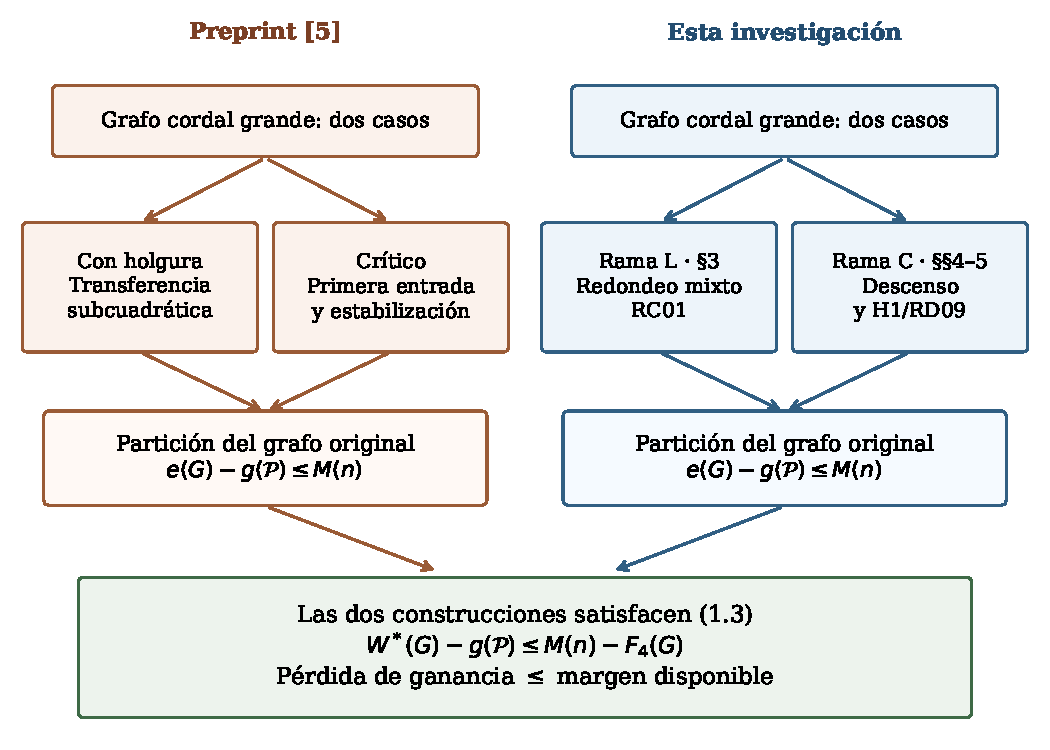
\includegraphics[width=.95\linewidth]{figures/fig1_presupuesto_comparado.pdf}
\caption{Comparación de mecanismos. El preprint [5] y esta investigación separan dos casos alternativos y construyen una partición que cumple (1.3). Las flechas indican implicaciones hacia la conclusión, no el paso de un régimen al otro. Los localizadores de la columna izquierda están en la Sección 8.}
\end{figure}

\Needspace{22\baselineskip}

{\def\LTcaptype{none} % do not increment counter
\begin{longtable}[c]{@{}
  >{\raggedright\arraybackslash}p{(\linewidth - 4\tabcolsep) * \real{0.3333}}
  >{\raggedright\arraybackslash}p{(\linewidth - 4\tabcolsep) * \real{0.3333}}
  >{\raggedright\arraybackslash}p{(\linewidth - 4\tabcolsep) * \real{0.3333}}@{}}
\toprule\noalign{}
\begin{minipage}[b]{\linewidth}\raggedright
Componente
\end{minipage} & \begin{minipage}[b]{\linewidth}\raggedright
Preprint {[}5{]}
\end{minipage} & \begin{minipage}[b]{\linewidth}\raggedright
Esta investigación
\end{minipage} \\
\midrule\noalign{}
\endhead
\bottomrule\noalign{}
\endlastfoot
Margen cuadrático & Transferencia, §§2 y 9 & Redondeo mixto, §3 \\
Camino de copias & Adaptación de Paper II, §6 & Transporte mixto y selección, Lema 4.1 \\
Localización & Primera entrada, §8 & Descenso desde el terminal, §4.2 \\
Construcción cercana & Coloración por listas, §3 & Clases equilibradas y candidatos, §5.3 \\
Cuentas estructurales & Estabilidad local, §5 & Testigo conservado y Teorema 6.1 \\
Conclusión extremal & Cota eventual, §9 & Teorema B y Corolario 6.2 \\
\end{longtable}
}

\textbf{Tabla 5.} Comparación de pasos y localizadores. No es una tabla de prioridad bibliográfica ni afirma que los antecedentes de cada paso sean exclusivos de un desarrollo.

La relación con la serie está documentada en el propio preprint {[}5{]}. Su introducción cita la cota fraccional de Paper II y el resultado split de Paper III; su Sección 6 atribuye a Paper II el esquema de copias, la selección por clases y el terminal split, y desarrolla la adaptación mixta. Esta procedencia no implica que todo paso de {[}5{]} sea consecuencia formal de la serie, del mismo modo que compartir esos antecedentes no identifica nuestros dos mecanismos críticos.

\subsubsection{8.1. El antecedente de defecto simplicial acotado}\label{el-antecedente-de-defecto-simplicial-acotado}

Okechukwu {[}15, Teorema 1.1{]} establece el máximo eventual para defecto fijo utilizado en el Teorema C. Coinciden la clase de grafos, la notación \(Q_s(n)\), los cuantificadores eventuales y la familia que alcanza la cota. Ese teorema también da una cota aditiva para todos los órdenes para \(\operatorname{cp}\) y clasifica los grafos de igualdad. Usamos su definición de defecto enraizado, incluida la cuantificación sobre cliques prescritas. La conclusión adicional de cota superior en el Teorema C es una partición con piezas de orden a lo sumo cuatro, demostrada mediante nuestra propia cadena formal; el máximo irrestricto no se presenta como una fórmula extremal nueva. Esta comparación de enunciados no afirma que el método de {[}15{]} sea incapaz de dar la restricción más fuerte sobre el orden de las piezas.

\Needspace{16\baselineskip}

{\def\LTcaptype{none} % do not increment counter
\begin{longtable}[c]{@{}
  >{\raggedright\arraybackslash}p{(\linewidth - 4\tabcolsep) * \real{0.3333}}
  >{\raggedright\arraybackslash}p{(\linewidth - 4\tabcolsep) * \real{0.3333}}
  >{\raggedright\arraybackslash}p{(\linewidth - 4\tabcolsep) * \real{0.3333}}@{}}
\toprule\noalign{}
\begin{minipage}[b]{\linewidth}\raggedright
Componente
\end{minipage} & \begin{minipage}[b]{\linewidth}\raggedright
Okechukwu {[}15{]}
\end{minipage} & \begin{minipage}[b]{\linewidth}\raggedright
Esta investigación
\end{minipage} \\
\midrule\noalign{}
\endhead
\bottomrule\noalign{}
\endlastfoot
Localización & Dual con signos, Teorema 3.3 & Descenso por copias, §4 \\
Transferencia & Haxell--Rödl, plantillas conjuntas, Lema 3.4 & Selección mixta de dos cuotas, §3 y Apéndice C \\
Construcción crítica & Coloración por listas y excepciones, §§4--5 & Raíz regularizada y candidatos, §5 \\
\end{longtable}
}

\textbf{Tabla 6.} Comparación adicional; {[}15{]} no se identifica con {[}5{]}.

El corte de orden en {[}15{]} requiere cuidado. Su Teorema 3.3 elige \(L\) en función de la precisión de localización, y el argumento de estabilidad utilizado por la Proposición 5.4 y el Teorema 1.1 aplica ese corte mediante el Lema 3.4. No fija \(L=4\). La elección explícita \(L=4\) que sigue a la prueba de {[}15, Teorema 1.3{]} demuestra su aproximación separada (1.5), no la cota exacta del Teorema 1.1. Así, nuestra conclusión con orden fijo cuatro refuerza la cota superior exacta enunciada; no se afirma que toda adaptación posible del método de {[}15{]} necesite cliques mayores.

Para conectar su transferencia con la Tabla 4, {[}15, Lema 3.4{]} proporciona \(q_L(G)\le q_L^*(G)+\zeta n^2\). Su partición fraccional exacta es equivalente al modelo de ganancia de §1.1, luego \(q_L^*=F_{\{3,\ldots,L\}}\). Esa cota paga el presupuesto cuando \(\zeta n^2\le M(n)-q_L^*(G)\). El lema de aproximación aislado no garantiza esa última condición: se utiliza en la rama que dispone del margen correspondiente.

La comparación de estabilidad tiene un alcance distinto. Nuestro Teorema 6.1 da una cota explícita lineal en el déficit integral bajo hipótesis cordales, y el Corolario 6.1a controla las piezas de particiones casi óptimas mediante la misma raíz. En {[}15{]}, el Teorema 1.3 da estabilidad estructural asintótica para una clase más amplia de defecto enraizado, mientras que el Corolario 5.5 da estabilidad por ediciones en forma \(\varepsilon\)--\(\delta\) para cada defecto fijo. El Teorema C no extiende automáticamente nuestra estabilidad cordal cuantitativa. En cuanto a los umbrales, §6.3 y C.3 dan una cota global explícita de tipo torre para los cordales. No es práctica y no debe confundirse con el umbral cercano \(4\cdot10^{12}\).

El término \(n/6+1/24\) que aparece en la prueba de {[}15, Teorema 3.3{]} también figura en nuestra calibración: en ambos casos \((2n+1)^2/24=n^2/6+n/6+1/24\). Proviene de la envolvente cuadrática continua; no es, por sí solo, el error del piso de \(M(n)\). El perfil entero de §6.7 conserva además ese piso. Los núcleos óptimos de {[}15, Corolario 1.2{]}, descritos por los enteros más cercanos a \((2n+1)/6\), coinciden con (6.4), incluido el empate cuando \(n\equiv1\pmod3\).

El preprint {[}5{]} tiene un desarrollo Lean público. Nuestra auditoría se refiere al corte propio y al veto descrito en §7; no es una afirmación de exclusividad de la formalización. Tampoco la forma aditiva para todos los órdenes distingue por sí sola los resultados: una cota eventual \(c_4\le M\), como la obtenida por la construcción de {[}5{]}, implica \(c_4\le M+b\) al absorber el rango finito restante, exactamente como en §6.3.

Se registra también el proyecto \emph{Clique Partitions of Split Graphs} de Henderson, Koerts, Roberge, Spirkl y Whitman, anunciado en preparación {[}16{]}. Consultada el 27 de septiembre de 2026, la página no enlaza un manuscrito; por eso no se le atribuyen resultados ni se afirma un solapamiento.

\subsubsection{8.2. Cota para todos los órdenes y gaps de empaquetamiento}\label{cota-para-todos-los-ordenes-y-gaps-de-empaquetamiento}

¿Vale \(c_4(G)\le M(n)\) para todo cordal y todo orden, es decir, puede tomarse \(b=0\) en el Teorema A? El umbral de esta prueba limita la demostración, no constituye evidencia de una excepción al enunciado. Para la familia completa sí se dispone de una construcción sin umbral: \(c_4(K_n)\le M(n)\) para todo \(n\ge0\), como se demuestra en el Apéndice D. A diferencia de \(\operatorname{cp}(K_n)=1\) para \(n\ge2\), esta afirmación exige controlar el tamaño de las piezas.

La demostración no necesita ni establece una cota lineal universal para el gap mixto \(W^*(G)-W(G)\), donde \(W(G)\) es la ganancia mixta entera óptima. Compara la pérdida de la construcción con el margen disponible en cada instancia. El orden de crecimiento general de ese gap se estudia por separado; no es una hipótesis de este paper.

Hay un resultado complementario para el \textbf{gap triangular} con número de clique acotado. Sean \(d\ge0\) entero y \(G\) cordal sin clique de orden \(d+2\). La biblioteca {\ttfamily\small BoundedCliqu\discretionary{\hbox{\ensuremath{\hookrightarrow}}}{}{}eGap}, incluida como anexo de fuentes separado y comprobada contra una compilación registrada distinta, demuestra que todo empaquetamiento fraccional triangular \(x\) satisface \[
\sum_T x_T\le \nu_3(G)+\left(10+\frac d2\right)n.
\tag{8.1a}
\] Aquí \(\nu_3(G)\) cuenta triángulos disjuntos por aristas; el objetivo fraccional cuenta también triángulos, sin el factor de ganancia dos. Tomar el óptimo da \(\nu_3^*(G)-\nu_3(G)\le(10+d/2)n\). Para \(d\) fijo, la pérdida es lineal; no se obtiene de ello una constante uniforme cuando crece el número de clique.

El enunciado formal es {\ttfamily\small BoundedCliqu\discretionary{\hbox{\ensuremath{\hookrightarrow}}}{}{}eGap.\discretionary{\hbox{\ensuremath{\hookrightarrow}}}{}{}chordal\_\discretionary{\hbox{\ensuremath{\hookrightarrow}}}{}{}gap\_\discretionary{\hbox{\ensuremath{\hookrightarrow}}}{}{}linear\_\discretionary{\hbox{\ensuremath{\hookrightarrow}}}{}{}cliqueFree}. Su prueba emplea una representación por subárboles y separa la masa de las piezas locales de la que atraviesa las uniones. Cada triángulo de esta última clase utiliza dos aristas de unión; sumar sus capacidades paga su masa con la mitad de la cuenta de esas aristas. La cota \(d\) controla esa cuenta y aporta el término \(dn/2\), además de la pérdida local \(10n\).

La misma biblioteca expresa la hipótesis mediante un árbol de cliques cuyas bolsas tienen a lo sumo \(d+1\) vértices. {\ttfamily\small exists\_\discretionary{\hbox{\ensuremath{\hookrightarrow}}}{}{}cliqueTree\_\discretionary{\hbox{\ensuremath{\hookrightarrow}}}{}{}width\_\discretionary{\hbox{\ensuremath{\hookrightarrow}}}{}{}le\_\discretionary{\hbox{\ensuremath{\hookrightarrow}}}{}{}iff\_\discretionary{\hbox{\ensuremath{\hookrightarrow}}}{}{}cliqueFree} demuestra, para cordales, la equivalencia con la exclusión de \(K_{d+2}\). Es la forma de anchura de árbol disponible en este desarrollo; no se afirma que Mathlib proporcione una definición general de \emph{treewidth} utilizada aquí. El resultado (8.1a) no acota el gap \textbf{mixto} de \(K_3/K_4\), ni sustituye el redondeo de la Sección 3.

\subsubsection{8.3. Una obstrucción cuantitativa para la limpieza de codegrado}\label{una-obstruccion-cuantitativa-para-la-limpieza-de-codegrado}

El umbral del Teorema 3.1 procede de la construcción con regularidad del Apéndice C. Un complemento formal, separado de esa prueba, permite acotar qué puede conseguirse mediante otra interfaz de limpieza. Es necesario distinguir ambos objetos: demostrar que una limpieza basta para redondear no demuestra que todo redondeador tenga que realizarla.

Fijemos \(\varepsilon>0\), \(\gamma\le1/2\) y una constante \(C_0\). Consideremos el siguiente contrato, llamado {\ttfamily\small CleanupAtWit\discretionary{\hbox{\ensuremath{\hookrightarrow}}}{}{}h} en el suplemento. Para todo grafo \(G\) de orden \(n\ge N_0\) y todo empaquetamiento fraccional mixto \(x\) cuya masa triangular sea al menos \(\varepsilon n^2/30-1\), exige otro empaquetamiento \(y\) sobre el mismo grafo con masa triangular al menos \(C_0\), pérdida de ganancia a lo sumo \(\varepsilon n^2/4\) y codegrado ponderado a lo sumo \(\gamma\). Este último codegrado es la suma de pesos de las copias que contienen simultáneamente dos aristas distintas del grafo.

\Needspace{9\baselineskip}

\textbf{Proposición 8.1 (límite de ese contrato).} Si \(N_0\) satisface el contrato anterior, \(t\ge4\) y \(7\varepsilon\le e^{-t}\), entonces \[
N_0>\exp(t^2/16).
\tag{8.2}
\] En particular, si \(\varepsilon\le1/(7e^{34})\), se tiene \(N_0>e^{72}\). La precisión es racional en la declaración Lean; las comparaciones exponenciales se realizan en los reales.

\textbf{Demostración.} Llamemos rígido a un grafo cuyas aristas pertenecen, cada una, a un único triángulo, sin copias de \(K_4\). Si tiene \(T\) triángulos, poner peso uno sobre cada uno da ganancia \(2T\). Dos aristas de un mismo triángulo sólo pueden recibir peso conjunto a través de esa copia. Por tanto, todo \(y\) de codegrado a lo sumo \(\gamma\) le asigna peso a lo sumo \(\gamma\), y su ganancia es a lo sumo \(2\gamma T\). La pérdida forzada es al menos \(2(1-\gamma)T\). Para un orden que satisfaga la hipótesis de masa, el contrato impone \[
2(1-\gamma)T\le\frac{\varepsilon}{4}n^2.
\tag{8.3}
\] Así, una limpieza uniforme de este tipo controla cuantitativamente la densidad de los sistemas rígidos, un problema de tipo \((6,3)\).

La construcción tripartita de Ruzsa--Szemerédi {[}18{]}, aplicada a un conjunto \(A\subseteq\{0,\ldots,M-1\}\) sin progresiones aritméticas de tres términos, da un grafo rígido de orden \(6M+3\) con al menos \((2M+1)|A|\) triángulos. La versión de la cota de Behrend {[}17{]} utilizada en Mathlib garantiza \(|A|\ge M\exp(-4\sqrt{\log M})\). Si \(7\varepsilon\le\exp(-4\sqrt{\log M})\) y \(M\ge1\), esa cuenta cumple la hipótesis de masa y contradice (8.3): el orden \(6M+3\) debe ser menor que \(N_0\).

Tomemos ahora \(M=\lfloor\exp(t^2/16)\rfloor\). Entonces \(M\ge1\), \(\log M\le t^2/16\) y \(4\sqrt{\log M}\le t\). Se aplica el párrafo anterior. Como \(\exp(t^2/16)<M+1\le6M+3\), resulta (8.2). Para \(t=34\), \(t^2/16=72.25>72\), lo que da la última afirmación. Las declaraciones {\ttfamily\small threshold\_\discretionary{\hbox{\ensuremath{\hookrightarrow}}}{}{}gt\_\discretionary{\hbox{\ensuremath{\hookrightarrow}}}{}{}exp} y {\ttfamily\small threshold\_\discretionary{\hbox{\ensuremath{\hookrightarrow}}}{}{}gt\_\discretionary{\hbox{\ensuremath{\hookrightarrow}}}{}{}exp\_\discretionary{\hbox{\ensuremath{\hookrightarrow}}}{}{}seventy\_\discretionary{\hbox{\ensuremath{\hookrightarrow}}}{}{}two}, de {\ttfamily\small FarExplorati\discretionary{\hbox{\ensuremath{\hookrightarrow}}}{}{}on.\discretionary{\hbox{\ensuremath{\hookrightarrow}}}{}{}CleanupRigid\discretionary{\hbox{\ensuremath{\hookrightarrow}}}{}{}Verdict}, formalizan estas cuentas usando la cota de Behrend de Mathlib.

Para \(t=\log(1/(7\varepsilon))\), (8.2) crece más deprisa que cualquier potencia fija de \(1/\varepsilon\); {\ttfamily\small threshold\_\discretionary{\hbox{\ensuremath{\hookrightarrow}}}{}{}superpolynom\discretionary{\hbox{\ensuremath{\hookrightarrow}}}{}{}ial} ofrece también esa formulación. Esto descarta un umbral polinómico para \textbf{este contrato}, no para cualquier prueba de Erdős 81. No demuestra que regularidad sea el único método posible, ni que se necesite una torre, ni que \(e^{72}\) sea una cota inferior del umbral del Teorema 3.1. El complemento demuestra la implicación limpieza \(\Rightarrow\) redondeo; para transportar su barrera a otro redondeador haría falta la implicación inversa o un adaptador cuantitativo.

\textbf{Qué cambia si se exige cordalidad.} Tanto {\ttfamily\small CodegreeClea\discretionary{\hbox{\ensuremath{\hookrightarrow}}}{}{}nupAt} como {\ttfamily\small UniformRound\discretionary{\hbox{\ensuremath{\hookrightarrow}}}{}{}ingTarget} cuantifican sobre todos los grafos, mientras que el ensamblaje de la rama lejana los utiliza sobre el grafo cordal original. La familia rígida anterior no da la misma obstrucción en esa clase. En efecto, sea \(G\) cordal, sin \(K_4\), con \(n\ge2\). En un orden de eliminación perfecto, cada vértice tiene a lo sumo dos vecinos posteriores; de otro modo, él y tres de esos vecinos formarían un \(K_4\). Al contar cada arista por su extremo anterior, los primeros \(n-2\) vértices contribuyen a lo sumo dos cada uno, el penúltimo a lo sumo una y el último ninguna. Por tanto, \[
e(G)\le2(n-2)+1=2n-3.
\tag{8.4}
\] Si además \(G\) es rígido, sus \(T\) triángulos son disjuntos por aristas. Así, \(3T\le e(G)\), y cualquier masa triangular fraccional factible es a lo sumo \(T\). Para que se cumpla la hipótesis de masa del contrato sería necesario que \[
\frac{\varepsilon n^2}{30}-1
\le T\le\frac{2n-3}{3}
\quad\Longrightarrow\quad n\le\frac{20}{\varepsilon}.
\tag{8.5}
\] La cancelación de los términos constantes explica el último umbral. Por encima de él, ningún cordal rígido satisface la hipótesis de masa. En particular, las instancias densas usadas para obtener la barrera superpolinómica no pueden ser cordales. No se afirma lo mismo de cada instancia pequeña o degenerada de la construcción tripartita.

Esta cuenta delimita el alcance de la obstrucción; no demuestra una limpieza cordal ni una cota superior \(O(1/\varepsilon)\) para su umbral. Tampoco se ha formalizado aquí una versión de la implicación limpieza--redondeo restringida a cordales. Estudiar ese contrato más débil es una cuestión distinta tanto de la barrera universal como del gap triangular con clique acotada de §8.2.

\subsection{Apéndice A. Correspondencia formal y reproducción}\label{apendice-a.-correspondencia-formal-y-reproduccion}

\subsubsection{A.1. Enunciados y comprobaciones}\label{a.1.-enunciados-y-comprobaciones}

En la tabla siguiente se omite el prefijo común {\ttfamily\small PaperIV}. Para cada fila, {\ttfamily\small Audit.\discretionary{\hbox{\ensuremath{\hookrightarrow}}}{}{}lean} imprime la huella fundacional; en la ejecución sobre el corte identificado sólo aparecen {\ttfamily\small propext}, {\ttfamily\small Classical.\discretionary{\hbox{\ensuremath{\hookrightarrow}}}{}{}choice} y {\ttfamily\small Quot.\discretionary{\hbox{\ensuremath{\hookrightarrow}}}{}{}sound}. {\ttfamily\small ConeAudit.\discretionary{\hbox{\ensuremath{\hookrightarrow}}}{}{}lean} examina las dependencias de los enunciados finales. La lista completa de fuentes compiladas y sus SHA-256 está en \nolinkurl{03_reproducibility/build_v1.0_20260927/SOURCES.json}; el mapa declaración por declaración está en la auditoría interna del autor, \nolinkurl{02_validation/01_INTERNAL_AUDITS/run_20260927_v1.0_f1769273dd2c/00_CONTROL/CLAIM_MAP.csv}. Los archivos anteriores {\ttfamily\small AUDIT\_\discretionary{\hbox{\ensuremath{\hookrightarrow}}}{}{}DECLARATIONS\discretionary{\hbox{\ensuremath{\hookrightarrow}}}{}{}.\discretionary{\hbox{\ensuremath{\hookrightarrow}}}{}{}tsv} y {\ttfamily\small AUDIT\_\discretionary{\hbox{\ensuremath{\hookrightarrow}}}{}{}SNAPSHOT.\discretionary{\hbox{\ensuremath{\hookrightarrow}}}{}{}json} siguen siendo registros históricos del draft, no evidencia de este corte.

{\def\LTcaptype{none} % do not increment counter
\begin{longtable}[c]{@{}
  >{\raggedright\arraybackslash}p{(\linewidth - 2\tabcolsep) * \real{0.5000}}
  >{\raggedright\arraybackslash}p{(\linewidth - 2\tabcolsep) * \real{0.5000}}@{}}
\toprule\noalign{}
\begin{minipage}[b]{\linewidth}\raggedright
Resultado
\end{minipage} & \begin{minipage}[b]{\linewidth}\raggedright
Declaración Lean
\end{minipage} \\
\midrule\noalign{}
\endhead
\bottomrule\noalign{}
\endlastfoot
Teorema A, forma aditiva & {\ttfamily\small Erdos81AllOr\discretionary{\hbox{\ensuremath{\hookrightarrow}}}{}{}ders.\discretionary{\hbox{\ensuremath{\hookrightarrow}}}{}{}erdos81\_\discretionary{\hbox{\ensuremath{\hookrightarrow}}}{}{}all\_\discretionary{\hbox{\ensuremath{\hookrightarrow}}}{}{}orders\_\discretionary{\hbox{\ensuremath{\hookrightarrow}}}{}{}additive} \\
Teorema B, cota superior & {\ttfamily\small Erdos81Uncon\discretionary{\hbox{\ensuremath{\hookrightarrow}}}{}{}ditional.\discretionary{\hbox{\ensuremath{\hookrightarrow}}}{}{}erdos81\_\discretionary{\hbox{\ensuremath{\hookrightarrow}}}{}{}cliquePartit\discretionary{\hbox{\ensuremath{\hookrightarrow}}}{}{}ion} \\
Teorema B, máximo & {\ttfamily\small PaperTheorem\discretionary{\hbox{\ensuremath{\hookrightarrow}}}{}{}s.\discretionary{\hbox{\ensuremath{\hookrightarrow}}}{}{}erdos81\_\discretionary{\hbox{\ensuremath{\hookrightarrow}}}{}{}max\_\discretionary{\hbox{\ensuremath{\hookrightarrow}}}{}{}eq} \\
Teorema 3.1 & {\ttfamily\small RC01Final.\discretionary{\hbox{\ensuremath{\hookrightarrow}}}{}{}rc01\_\discretionary{\hbox{\ensuremath{\hookrightarrow}}}{}{}uniformRound\discretionary{\hbox{\ensuremath{\hookrightarrow}}}{}{}ingTarget} \\
Corolario 3.5 & {\ttfamily\small FarRegimeAll\discretionary{\hbox{\ensuremath{\hookrightarrow}}}{}{}Graphs.\discretionary{\hbox{\ensuremath{\hookrightarrow}}}{}{}farRegime\_\discretionary{\hbox{\ensuremath{\hookrightarrow}}}{}{}cliquePartit\discretionary{\hbox{\ensuremath{\hookrightarrow}}}{}{}ion\_\discretionary{\hbox{\ensuremath{\hookrightarrow}}}{}{}allGraphs} \\
Dicotomía (1.5) & {\ttfamily\small HybridDichot\discretionary{\hbox{\ensuremath{\hookrightarrow}}}{}{}omy.\discretionary{\hbox{\ensuremath{\hookrightarrow}}}{}{}chordal\_\discretionary{\hbox{\ensuremath{\hookrightarrow}}}{}{}far\_\discretionary{\hbox{\ensuremath{\hookrightarrow}}}{}{}or\_\discretionary{\hbox{\ensuremath{\hookrightarrow}}}{}{}nearStructur\discretionary{\hbox{\ensuremath{\hookrightarrow}}}{}{}e} \\
Teorema 5.0, ventana reforzada & {\ttfamily\small NearH1LocalC\discretionary{\hbox{\ensuremath{\hookrightarrow}}}{}{}onstructor.\discretionary{\hbox{\ensuremath{\hookrightarrow}}}{}{}exists\_\discretionary{\hbox{\ensuremath{\hookrightarrow}}}{}{}near\_\discretionary{\hbox{\ensuremath{\hookrightarrow}}}{}{}partition\_\discretionary{\hbox{\ensuremath{\hookrightarrow}}}{}{}paid\_\discretionary{\hbox{\ensuremath{\hookrightarrow}}}{}{}by\_\discretionary{\hbox{\ensuremath{\hookrightarrow}}}{}{}root\_\discretionary{\hbox{\ensuremath{\hookrightarrow}}}{}{}sharp} \\
Teorema 5.0, interfaz anterior & {\ttfamily\small NearH1LocalC\discretionary{\hbox{\ensuremath{\hookrightarrow}}}{}{}onstructor.\discretionary{\hbox{\ensuremath{\hookrightarrow}}}{}{}exists\_\discretionary{\hbox{\ensuremath{\hookrightarrow}}}{}{}near\_\discretionary{\hbox{\ensuremath{\hookrightarrow}}}{}{}partition\_\discretionary{\hbox{\ensuremath{\hookrightarrow}}}{}{}paid\_\discretionary{\hbox{\ensuremath{\hookrightarrow}}}{}{}by\_\discretionary{\hbox{\ensuremath{\hookrightarrow}}}{}{}root} \\
Corolario 5.4, tamaño y densidad & {\ttfamily\small NearCritical\discretionary{\hbox{\ensuremath{\hookrightarrow}}}{}{}Dichotomy.\discretionary{\hbox{\ensuremath{\hookrightarrow}}}{}{}chordal\_\discretionary{\hbox{\ensuremath{\hookrightarrow}}}{}{}far\_\discretionary{\hbox{\ensuremath{\hookrightarrow}}}{}{}or\_\discretionary{\hbox{\ensuremath{\hookrightarrow}}}{}{}criticalRoot}, {\ttfamily\small chordal\_\discretionary{\hbox{\ensuremath{\hookrightarrow}}}{}{}far\_\discretionary{\hbox{\ensuremath{\hookrightarrow}}}{}{}or\_\discretionary{\hbox{\ensuremath{\hookrightarrow}}}{}{}edge\_\discretionary{\hbox{\ensuremath{\hookrightarrow}}}{}{}density} \\
Optimalidad del coeficiente cuadrático & {\ttfamily\small SharpConstan\discretionary{\hbox{\ensuremath{\hookrightarrow}}}{}{}tOptimality.\discretionary{\hbox{\ensuremath{\hookrightarrow}}}{}{}erdos81\_\discretionary{\hbox{\ensuremath{\hookrightarrow}}}{}{}quadratic\_\discretionary{\hbox{\ensuremath{\hookrightarrow}}}{}{}constant\_\discretionary{\hbox{\ensuremath{\hookrightarrow}}}{}{}optimal}, {\ttfamily\small erdos81\_\discretionary{\hbox{\ensuremath{\hookrightarrow}}}{}{}quadratic\_\discretionary{\hbox{\ensuremath{\hookrightarrow}}}{}{}constant\_\discretionary{\hbox{\ensuremath{\hookrightarrow}}}{}{}isLeast} \\
Teorema 6.1, forma fuerte & {\ttfamily\small IntegralStab\discretionary{\hbox{\ensuremath{\hookrightarrow}}}{}{}ility.\discretionary{\hbox{\ensuremath{\hookrightarrow}}}{}{}chordal\_\discretionary{\hbox{\ensuremath{\hookrightarrow}}}{}{}linear\_\discretionary{\hbox{\ensuremath{\hookrightarrow}}}{}{}stability\_\discretionary{\hbox{\ensuremath{\hookrightarrow}}}{}{}sixteen} \\
Teorema 6.1, interfaz anterior & {\ttfamily\small IntegralStab\discretionary{\hbox{\ensuremath{\hookrightarrow}}}{}{}ility.\discretionary{\hbox{\ensuremath{\hookrightarrow}}}{}{}chordal\_\discretionary{\hbox{\ensuremath{\hookrightarrow}}}{}{}linear\_\discretionary{\hbox{\ensuremath{\hookrightarrow}}}{}{}stability} \\
Corolario 6.1a & {\ttfamily\small RootPartitio\discretionary{\hbox{\ensuremath{\hookrightarrow}}}{}{}nStability.\discretionary{\hbox{\ensuremath{\hookrightarrow}}}{}{}chordal\_\discretionary{\hbox{\ensuremath{\hookrightarrow}}}{}{}partition\_\discretionary{\hbox{\ensuremath{\hookrightarrow}}}{}{}stability} \\
Identidad (6.7b) & {\ttfamily\small RootPartitio\discretionary{\hbox{\ensuremath{\hookrightarrow}}}{}{}nStability.\discretionary{\hbox{\ensuremath{\hookrightarrow}}}{}{}sum\_\discretionary{\hbox{\ensuremath{\hookrightarrow}}}{}{}rootPieceDef\discretionary{\hbox{\ensuremath{\hookrightarrow}}}{}{}ect\_\discretionary{\hbox{\ensuremath{\hookrightarrow}}}{}{}eq} \\
Corolario 6.2 & {\ttfamily\small ExtremalClas\discretionary{\hbox{\ensuremath{\hookrightarrow}}}{}{}sification.\discretionary{\hbox{\ensuremath{\hookrightarrow}}}{}{}chordal\_\discretionary{\hbox{\ensuremath{\hookrightarrow}}}{}{}extremal\_\discretionary{\hbox{\ensuremath{\hookrightarrow}}}{}{}classificati\discretionary{\hbox{\ensuremath{\hookrightarrow}}}{}{}on} \\
Proposición 6.3 & {\ttfamily\small SplitMixedGa\discretionary{\hbox{\ensuremath{\hookrightarrow}}}{}{}p.\discretionary{\hbox{\ensuremath{\hookrightarrow}}}{}{}mixed\_\discretionary{\hbox{\ensuremath{\hookrightarrow}}}{}{}gap\_\discretionary{\hbox{\ensuremath{\hookrightarrow}}}{}{}zero} junto con la construcción acotada en {\ttfamily\small SplitComplet\discretionary{\hbox{\ensuremath{\hookrightarrow}}}{}{}eSharpValue} \\
\end{longtable}
}

\textbf{Tabla 7.} Declaraciones finales. La tabla de módulos de la Sección 7 localiza la implementación; esta tabla identifica qué enunciado se audita.

La ejecución local combinada comprobó \nolinkurl{PaperIV/Audit.lean} y \nolinkurl{PaperIV/ConeAudit.lean} como targets separados, junto con {\ttfamily\small PaperIV} y los demás targets de {\ttfamily\small RUN\_\discretionary{\hbox{\ensuremath{\hookrightarrow}}}{}{}META.\discretionary{\hbox{\ensuremath{\hookrightarrow}}}{}{}json}. La versión exacta de Lean está en {\ttfamily\small lean-\discretionary{\hbox{\ensuremath{\hookrightarrow}}}{}{}toolchain}; las revisiones de las dependencias, en {\ttfamily\small lake-\discretionary{\hbox{\ensuremath{\hookrightarrow}}}{}{}manifest.\discretionary{\hbox{\ensuremath{\hookrightarrow}}}{}{}json}. Un build del agregado sirve como comprobación adicional de integración, pero no sustituye la inspección de los enunciados ni sus huellas. El corte de fuentes es local y está identificado; la auditoría interna del autor concluyó y quedan pendientes la revisión adversarial y el enlace público permanente.

\textbf{Definiciones literales.} Los fragmentos siguientes reproducen las definiciones y las cabeceras de los teoremas, omitiendo sus demostraciones, no sus hipótesis. En el primer fragmento el espacio es {\ttfamily\small SimpleGraph}; en los tres siguientes es {\ttfamily\small PaperIV.\discretionary{\hbox{\ensuremath{\hookrightarrow}}}{}{}FarRounding}, con \(V\) finito, igualdad decidible y adyacencia decidible para \(G\). La última definición está en {\ttfamily\small PaperIV}. Los nombres de los espacios se conservan en el archivo complementario de extractos.

\begin{quote}\footnotesize\ttfamily\raggedright
def IsChordal (G : SimpleGraph V) : Prop :=\par
  \(\forall\) \(\{\!\{\)v : V\(\}\!\}\) (c : G.Walk v v), c.IsCycle \(\to\) 4 \(\le\) c.length \(\to\)\par
    \(\exists\) x y : V, x \(\in\) c.support \(\land\) y \(\in\) c.support \(\land\) G.Adj x y \(\land\) s(x, y) \(\notin\) c.edges\par
\end{quote}

\begin{quote}\footnotesize\ttfamily\raggedright
def pairs (K : Finset V) : Finset (Sym2 V) := K.sym2.filter fun e => \(\neg\) e.IsDiag\par
\par
structure CliquePartition where\par
  pieces : Finset (Finset V)\par
  isClique : \(\forall\) K \(\in\) pieces, \(\forall\) a \(\in\) K, \(\forall\) b \(\in\) K, a \(\ne\) b \(\to\) G.Adj a b\par
  two\_le\_card : \(\forall\) K \(\in\) pieces, 2 \(\le\) K.card\par
  edgeDisjoint : \(\forall\) K \(\in\) pieces, \(\forall\) L \(\in\) pieces, K \(\ne\) L \(\to\) Disjoint (pairs K) (pairs L)\par
  covers : pieces.biUnion pairs = G.edgeFinset\par
\par
def CliquePartition.size (Q : CliquePartition G) : \(\mathbb N\) := Q.pieces.card\par
\par
def CliquePartition.OrderAtMost (Q : CliquePartition G) (r : \(\mathbb N\)) : Prop :=\par
  \(\forall\) K \(\in\) Q.pieces, K.card \(\le\) r\par
\end{quote}

\begin{quote}\footnotesize\ttfamily\raggedright
def targetSize (n : \(\mathbb N\)) : \(\mathbb N\) := n * (n + 1) / 6\par
\end{quote}

La división de naturales implementa el piso de \(M(n)\). El símbolo expositivo \(c_4\) designa el mínimo sobre esas particiones con \texttt{OrderAtMost\ 4}; el enunciado exportado no presupone una función mínimo, sino que entrega directamente una partición testigo. La cordalidad de {\ttfamily\small FarRounding} es un alias literal de la definición por ciclos anterior.

\textbf{Teoremas exportados.} En {\ttfamily\small PaperIV.\discretionary{\hbox{\ensuremath{\hookrightarrow}}}{}{}Erdos81AllOr\discretionary{\hbox{\ensuremath{\hookrightarrow}}}{}{}ders} y {\ttfamily\small PaperIV.\discretionary{\hbox{\ensuremath{\hookrightarrow}}}{}{}Erdos81Uncon\discretionary{\hbox{\ensuremath{\hookrightarrow}}}{}{}ditional}, respectivamente, las cabeceras exactas son:

\begin{quote}\footnotesize\ttfamily\raggedright
theorem erdos81\_all\_orders\_additive :\par
    \(\exists\) b : \(\mathbb N\), \(\forall\) (n : \(\mathbb N\)) (G : SimpleGraph (Fin n)) [DecidableRel G.Adj],\par
      PaperIV.FarRounding.IsChordal G \(\to\)\par
        \(\exists\) Q : CliquePartition G, Q.OrderAtMost 4 \(\land\) Q.size \(\le\) PaperIV.targetSize n + b\par
\end{quote}

\begin{quote}\footnotesize\ttfamily\raggedright
theorem erdos81\_cliquePartition :\par
    \(\exists\) N : \(\mathbb N\), \(\forall\) n : \(\mathbb N\), N \(\le\) n \(\to\) \(\forall\) (G : SimpleGraph (Fin n)) [DecidableRel G.Adj],\par
      PaperIV.FarRounding.IsChordal G \(\to\)\par
        \(\exists\) Q : CliquePartition G, Q.OrderAtMost 4 \(\land\) Q.size \(\le\) targetSize n\par
\end{quote}

Estas cabeceras permiten comprobar el orden de cuantificadores y la cobertura exacta sin inferirlos del nombre del teorema. La auditoría adjunta no contiene {\ttfamily\small sorryAx} entre los axiomas de las declaraciones examinadas. El informe complementario distingue esa comprobación transitiva de la búsqueda textual de {\ttfamily\small native\_\discretionary{\hbox{\ensuremath{\hookrightarrow}}}{}{}decide} en las fuentes del proyecto y de una reconstrucción completa de las dependencias.

\subsubsection{A.2. Contratos intermedios de las pruebas}\label{a.2.-contratos-intermedios-de-las-pruebas}

\textbf{Alcance de la demostración escrita.} Las derivaciones finitas de la tabla siguiente se resumen, sin desarrollarse por completo en este manuscrito. Las fuentes Lean congeladas contienen las pruebas correspondientes; un build exitoso verifica sus derivaciones formales, no la suficiencia de su exposición. La primera auditoría externa dejó abierta su rederivación matemática independiente. Siguen siendo obligaciones explícitas de revisión, no hipótesis adicionales de los teoremas.

\Needspace{24\baselineskip}

{\def\LTcaptype{none} % do not increment counter
\begin{longtable}[c]{@{}
  >{\raggedright\arraybackslash}p{(\linewidth - 2\tabcolsep) * \real{0.5000}}
  >{\raggedright\arraybackslash}p{(\linewidth - 2\tabcolsep) * \real{0.5000}}@{}}
\toprule\noalign{}
\begin{minipage}[b]{\linewidth}\raggedright
Ubicación
\end{minipage} & \begin{minipage}[b]{\linewidth}\raggedright
Derivación no desarrollada por completo en la prosa
\end{minipage} \\
\midrule\noalign{}
\endhead
\bottomrule\noalign{}
\endlastfoot
§5.1, (5.4) y (5.7) & Estimaciones de masa, grado, paleta y anchura tras regularizar \\
C.2, (3.8) y (3.10) & Conteos de descarte y retención con las convenciones de partición \\
§3.2 y C.2 & Cotas inferiores de fibras desde pares regulares y su normalización \\
C.3, Tabla C.1 & Dominación numérica de las constantes del nibble e iteraciones de la torre \\
E.1 & Cotas de normalización previas al constructor terminal \\
E.1, (E.2b) y (E.2d) & Estimaciones terminales y presupuesto de tres casos \\
D.1 & Construcciones de marcos Bose/Skolem que sustentan la tabla de residuos \\
\end{longtable}
}

El nibble importado de Paper III y las construcciones clásicas de diseños conservan sus referencias indicadas. El mapa de fuentes siguiente localiza las implementaciones formales; no sustituye esas derivaciones por nombres de teoremas.

El nibble de rango acotado se reutiliza mediante {\ttfamily\small PaperIIISlac\discretionary{\hbox{\ensuremath{\hookrightarrow}}}{}{}kNibbleAdapt\discretionary{\hbox{\ensuremath{\hookrightarrow}}}{}{}er.\discretionary{\hbox{\ensuremath{\hookrightarrow}}}{}{}boundedRankN\discretionary{\hbox{\ensuremath{\hookrightarrow}}}{}{}ibbleAt}. La construcción de las dos cuotas está en {\ttfamily\small MarkedQuotaS\discretionary{\hbox{\ensuremath{\hookrightarrow}}}{}{}lackGate.\discretionary{\hbox{\ensuremath{\hookrightarrow}}}{}{}slackMarkedQ\discretionary{\hbox{\ensuremath{\hookrightarrow}}}{}{}uotaNibbleAt\discretionary{\hbox{\ensuremath{\hookrightarrow}}}{}{}\_\discretionary{\hbox{\ensuremath{\hookrightarrow}}}{}{}proved}; el emparejamiento de soportes triangulares y su realización física están en {\ttfamily\small MarkedQuotaP\discretionary{\hbox{\ensuremath{\hookrightarrow}}}{}{}airing} y {\ttfamily\small JointTwoQuot\discretionary{\hbox{\ensuremath{\hookrightarrow}}}{}{}aPhysical}. La escala conjunta de codegrado corresponde a {\ttfamily\small RC01CleanedG\discretionary{\hbox{\ensuremath{\hookrightarrow}}}{}{}ate.\discretionary{\hbox{\ensuremath{\hookrightarrow}}}{}{}cleanedPacki\discretionary{\hbox{\ensuremath{\hookrightarrow}}}{}{}ng\_\discretionary{\hbox{\ensuremath{\hookrightarrow}}}{}{}joint\_\discretionary{\hbox{\ensuremath{\hookrightarrow}}}{}{}codegree\_\discretionary{\hbox{\ensuremath{\hookrightarrow}}}{}{}le\_\discretionary{\hbox{\ensuremath{\hookrightarrow}}}{}{}of\_\discretionary{\hbox{\ensuremath{\hookrightarrow}}}{}{}served\_\discretionary{\hbox{\ensuremath{\hookrightarrow}}}{}{}patterns}. Los perfiles tienen masa a lo sumo \(t^2\), no uno: es la normalización física de {\ttfamily\small RC01PatternM\discretionary{\hbox{\ensuremath{\hookrightarrow}}}{}{}assScale}.

Para el camino mixto, {\ttfamily\small VertexCopyMo\discretionary{\hbox{\ensuremath{\hookrightarrow}}}{}{}notone.\discretionary{\hbox{\ensuremath{\hookrightarrow}}}{}{}two\_\discretionary{\hbox{\ensuremath{\hookrightarrow}}}{}{}mul\_\discretionary{\hbox{\ensuremath{\hookrightarrow}}}{}{}F4\_\discretionary{\hbox{\ensuremath{\hookrightarrow}}}{}{}le\_\discretionary{\hbox{\ensuremath{\hookrightarrow}}}{}{}add} prueba la desigualdad de las dos direcciones. {\ttfamily\small VertexCopyGa\discretionary{\hbox{\ensuremath{\hookrightarrow}}}{}{}te} selecciona el paso y su potencial finito; {\ttfamily\small GatedTermina\discretionary{\hbox{\ensuremath{\hookrightarrow}}}{}{}lSplit.\discretionary{\hbox{\ensuremath{\hookrightarrow}}}{}{}exists\_\discretionary{\hbox{\ensuremath{\hookrightarrow}}}{}{}split\_\discretionary{\hbox{\ensuremath{\hookrightarrow}}}{}{}terminal\_\discretionary{\hbox{\ensuremath{\hookrightarrow}}}{}{}symmetrizati\discretionary{\hbox{\ensuremath{\hookrightarrow}}}{}{}onPath} entrega la sucesión completa. La cuenta local se construye en {\ttfamily\small NearH1Window\discretionary{\hbox{\ensuremath{\hookrightarrow}}}{}{}Accounts}, antes de importarla en {\ttfamily\small NearH1Locali\discretionary{\hbox{\ensuremath{\hookrightarrow}}}{}{}zation}. Esta dirección de dependencias corresponde al orden lógico explicado en el Lema 4.2.

La extracción de la clique y la calibración están en {\ttfamily\small ChordalCoreM\discretionary{\hbox{\ensuremath{\hookrightarrow}}}{}{}issing} y {\ttfamily\small NearH1Calibr\discretionary{\hbox{\ensuremath{\hookrightarrow}}}{}{}atedRoot}. {\ttfamily\small Regularizati\discretionary{\hbox{\ensuremath{\hookrightarrow}}}{}{}on}, {\ttfamily\small Regularizati\discretionary{\hbox{\ensuremath{\hookrightarrow}}}{}{}onBounds} y {\ttfamily\small RegularizedR\discretionary{\hbox{\ensuremath{\hookrightarrow}}}{}{}ootGoal} prueban las propiedades de la raíz que utiliza {\ttfamily\small RootRegulari\discretionary{\hbox{\ensuremath{\hookrightarrow}}}{}{}zationBridge}. Finalmente, {\ttfamily\small NearH1PhaseI}, {\ttfamily\small RD09FactorCa\discretionary{\hbox{\ensuremath{\hookrightarrow}}}{}{}ndidateMomen\discretionary{\hbox{\ensuremath{\hookrightarrow}}}{}{}ts} y {\ttfamily\small RD09FactorCa\discretionary{\hbox{\ensuremath{\hookrightarrow}}}{}{}ndidateAvera\discretionary{\hbox{\ensuremath{\hookrightarrow}}}{}{}ge} producen las dos cuentas; {\ttfamily\small NearH1FinalA\discretionary{\hbox{\ensuremath{\hookrightarrow}}}{}{}ssembly} las une usando la misma primera asignación y sus enlaces ocupados. No se aplica la segunda fase a una copia independiente de los recursos.

El Teorema 5.0 tiene una forma reforzada, {\ttfamily\small NearH1LocalC\discretionary{\hbox{\ensuremath{\hookrightarrow}}}{}{}onstructor.\discretionary{\hbox{\ensuremath{\hookrightarrow}}}{}{}exists\_\discretionary{\hbox{\ensuremath{\hookrightarrow}}}{}{}near\_\discretionary{\hbox{\ensuremath{\hookrightarrow}}}{}{}partition\_\discretionary{\hbox{\ensuremath{\hookrightarrow}}}{}{}paid\_\discretionary{\hbox{\ensuremath{\hookrightarrow}}}{}{}by\_\discretionary{\hbox{\ensuremath{\hookrightarrow}}}{}{}root\_\discretionary{\hbox{\ensuremath{\hookrightarrow}}}{}{}sharp}, que añade \(|3|R|-n|\le n/50\) al constructor físico; la interfaz anterior {\ttfamily\small exists\_\discretionary{\hbox{\ensuremath{\hookrightarrow}}}{}{}near\_\discretionary{\hbox{\ensuremath{\hookrightarrow}}}{}{}partition\_\discretionary{\hbox{\ensuremath{\hookrightarrow}}}{}{}paid\_\discretionary{\hbox{\ensuremath{\hookrightarrow}}}{}{}by\_\discretionary{\hbox{\ensuremath{\hookrightarrow}}}{}{}root} se conserva como corolario. La reserva reforzada de (5.15a) se conserva para ese mismo testigo en {\ttfamily\small NearStructur\discretionary{\hbox{\ensuremath{\hookrightarrow}}}{}{}eWitness.\discretionary{\hbox{\ensuremath{\hookrightarrow}}}{}{}accounts\_\discretionary{\hbox{\ensuremath{\hookrightarrow}}}{}{}count\_\discretionary{\hbox{\ensuremath{\hookrightarrow}}}{}{}le\_\discretionary{\hbox{\ensuremath{\hookrightarrow}}}{}{}improved}; {\ttfamily\small IntegralStab\discretionary{\hbox{\ensuremath{\hookrightarrow}}}{}{}ility.\discretionary{\hbox{\ensuremath{\hookrightarrow}}}{}{}chordal\_\discretionary{\hbox{\ensuremath{\hookrightarrow}}}{}{}linear\_\discretionary{\hbox{\ensuremath{\hookrightarrow}}}{}{}stability\_\discretionary{\hbox{\ensuremath{\hookrightarrow}}}{}{}sixteen} y {\ttfamily\small RootPartitio\discretionary{\hbox{\ensuremath{\hookrightarrow}}}{}{}nStability.\discretionary{\hbox{\ensuremath{\hookrightarrow}}}{}{}chordal\_\discretionary{\hbox{\ensuremath{\hookrightarrow}}}{}{}partition\_\discretionary{\hbox{\ensuremath{\hookrightarrow}}}{}{}stability} la utilizan sin recombinar raíces ni packings. La selección cíclica de la fase I está en {\ttfamily\small RD09PaddedL1\discretionary{\hbox{\ensuremath{\hookrightarrow}}}{}{}Mass}; la última evaluación de la fase II, en {\ttfamily\small H1ImprovedCo\discretionary{\hbox{\ensuremath{\hookrightarrow}}}{}{}nstants.\discretionary{\hbox{\ensuremath{\hookrightarrow}}}{}{}l10\_\discretionary{\hbox{\ensuremath{\hookrightarrow}}}{}{}of\_\discretionary{\hbox{\ensuremath{\hookrightarrow}}}{}{}raw\_\discretionary{\hbox{\ensuremath{\hookrightarrow}}}{}{}rd09L2}. Los regímenes del comparador de (5.1a) se comprueban en {\ttfamily\small SplitCompara\discretionary{\hbox{\ensuremath{\hookrightarrow}}}{}{}torResidual.\discretionary{\hbox{\ensuremath{\hookrightarrow}}}{}{}residual\_\discretionary{\hbox{\ensuremath{\hookrightarrow}}}{}{}sq\_\discretionary{\hbox{\ensuremath{\hookrightarrow}}}{}{}le\_\discretionary{\hbox{\ensuremath{\hookrightarrow}}}{}{}of\_\discretionary{\hbox{\ensuremath{\hookrightarrow}}}{}{}near\_\discretionary{\hbox{\ensuremath{\hookrightarrow}}}{}{}split\_\discretionary{\hbox{\ensuremath{\hookrightarrow}}}{}{}universal}. La reserva (6.12) es {\ttfamily\small ReserveIdent\discretionary{\hbox{\ensuremath{\hookrightarrow}}}{}{}ity.\discretionary{\hbox{\ensuremath{\hookrightarrow}}}{}{}targetSize\_\discretionary{\hbox{\ensuremath{\hookrightarrow}}}{}{}eq\_\discretionary{\hbox{\ensuremath{\hookrightarrow}}}{}{}baseline\_\discretionary{\hbox{\ensuremath{\hookrightarrow}}}{}{}add\_\discretionary{\hbox{\ensuremath{\hookrightarrow}}}{}{}reserve}; la contracción mejorada corresponde a {\ttfamily\small NearThreshol\discretionary{\hbox{\ensuremath{\hookrightarrow}}}{}{}dSensitivity\discretionary{\hbox{\ensuremath{\hookrightarrow}}}{}{}.\discretionary{\hbox{\ensuremath{\hookrightarrow}}}{}{}descent\_\discretionary{\hbox{\ensuremath{\hookrightarrow}}}{}{}threshold\_\discretionary{\hbox{\ensuremath{\hookrightarrow}}}{}{}maximal\_\discretionary{\hbox{\ensuremath{\hookrightarrow}}}{}{}barrier} y {\ttfamily\small near\_\discretionary{\hbox{\ensuremath{\hookrightarrow}}}{}{}threshold\_\discretionary{\hbox{\ensuremath{\hookrightarrow}}}{}{}binding}. Los resultados de geometría crítica están en {\ttfamily\small NearRootWind\discretionary{\hbox{\ensuremath{\hookrightarrow}}}{}{}ow}, {\ttfamily\small NearEdgeDens\discretionary{\hbox{\ensuremath{\hookrightarrow}}}{}{}ity} y {\ttfamily\small NearCritical\discretionary{\hbox{\ensuremath{\hookrightarrow}}}{}{}Dichotomy}.

Los incrementos de esta revisión tienen entradas públicas separadas. El Teorema C y su máximo son {\ttfamily\small PaperIV.\discretionary{\hbox{\ensuremath{\hookrightarrow}}}{}{}DefectSharpP\discretionary{\hbox{\ensuremath{\hookrightarrow}}}{}{}ublication.\discretionary{\hbox{\ensuremath{\hookrightarrow}}}{}{}rooted\_\discretionary{\hbox{\ensuremath{\hookrightarrow}}}{}{}defect\_\discretionary{\hbox{\ensuremath{\hookrightarrow}}}{}{}eventual} y {\ttfamily\small rooted\_\discretionary{\hbox{\ensuremath{\hookrightarrow}}}{}{}defect\_\discretionary{\hbox{\ensuremath{\hookrightarrow}}}{}{}maximum}; la Proposición D.2 es {\ttfamily\small order\_\discretionary{\hbox{\ensuremath{\hookrightarrow}}}{}{}three\_\discretionary{\hbox{\ensuremath{\hookrightarrow}}}{}{}insufficient} en el mismo espacio. La cuenta completa (3.11) corresponde a {\ttfamily\small E17Bridge.\discretionary{\hbox{\ensuremath{\hookrightarrow}}}{}{}improved\_\discretionary{\hbox{\ensuremath{\hookrightarrow}}}{}{}far\_\discretionary{\hbox{\ensuremath{\hookrightarrow}}}{}{}loss\_\discretionary{\hbox{\ensuremath{\hookrightarrow}}}{}{}explicit}. El Corolario 3.5 con umbral explícito es {\ttfamily\small E17Bridge.\discretionary{\hbox{\ensuremath{\hookrightarrow}}}{}{}ExplicitAsse\discretionary{\hbox{\ensuremath{\hookrightarrow}}}{}{}mbly.\discretionary{\hbox{\ensuremath{\hookrightarrow}}}{}{}farRegime\_\discretionary{\hbox{\ensuremath{\hookrightarrow}}}{}{}allGraphs\_\discretionary{\hbox{\ensuremath{\hookrightarrow}}}{}{}explicit}. Finalmente, {\ttfamily\small PaperIV.\discretionary{\hbox{\ensuremath{\hookrightarrow}}}{}{}ExplicitThre\discretionary{\hbox{\ensuremath{\hookrightarrow}}}{}{}shold.\discretionary{\hbox{\ensuremath{\hookrightarrow}}}{}{}erdos81\_\discretionary{\hbox{\ensuremath{\hookrightarrow}}}{}{}sharp\_\discretionary{\hbox{\ensuremath{\hookrightarrow}}}{}{}explicit} y {\ttfamily\small erdos81\_\discretionary{\hbox{\ensuremath{\hookrightarrow}}}{}{}all\_\discretionary{\hbox{\ensuremath{\hookrightarrow}}}{}{}orders\_\discretionary{\hbox{\ensuremath{\hookrightarrow}}}{}{}bounded\_\discretionary{\hbox{\ensuremath{\hookrightarrow}}}{}{}additive} entregan el resultado global con la torre de §6.3. Sus nombres son identificadores de declaraciones, no hipótesis nuevas.

El enlace B7 se audita mediante {\ttfamily\small E17.\discretionary{\hbox{\ensuremath{\hookrightarrow}}}{}{}ExplicitFarA\discretionary{\hbox{\ensuremath{\hookrightarrow}}}{}{}udit}. Reutiliza las constantes numéricas de {\ttfamily\small E18} y {\ttfamily\small E19}, pero construye el empaquetamiento mediante la limpieza mejorada: la auditoría exige sus dos cuentas en el cono y excluye los antiguos teoremas finales de existencia. Ese target pasó en la ejecución local combinada del corte identificado; la auditoría interna del autor revisó su log y sus hipótesis, con las limitaciones consignadas en el informe.

\subsubsection{A.3. Límites del resultado}\label{a.3.-limites-del-resultado}

No se demuestra un gap fraccionario--integral \(O(n)\) para todo cordal. Tampoco se afirma que toda demostración deba pasar por copias, regularización o un constructor particular. La cota eventual no resuelve si \(b=0\) en el Teorema A: esa igualdad conservaría el término \(n/6\) contenido en \(M(n)\), no lo eliminaría.

Las comprobaciones experimentales de órdenes pequeños no se usan como premisas. Su documentación, incluidos los requisitos de completitud y certificación, pertenece al registro de investigación separado.

La biblioteca de árboles de cliques conserva contraejemplos a formulaciones sin las hipótesis adecuadas: una hoja no equivale por sí sola a un único vértice simplicial, y las afirmaciones sobre separadores deben tratar las bolsas repetidas y los casos degenerados. Estos resultados delimitan el uso de esa biblioteca; no añaden supuestos al teorema principal.

\subsection{Apéndice B. Herramientas de construcción complementarias}\label{apendice-b.-herramientas-de-construccion-complementarias}

\subsubsection{B.1. Absorción compatible con presupuesto}\label{b.1.-absorcion-compatible-con-presupuesto}

La construcción cercana no es la única interfaz que convierte recursos disponibles en ganancia. Un emparejamiento perfecto sobre un conjunto par \(U\), junto con un anfitrión común \(z\), absorbe todos los enlaces \(zu\) mediante triángulos: cada pareja usa dos de esos enlaces y una base de \(G[U]\).

Supongamos que \[
d_{G[U]}(v)\ge |U|/2+t\qquad(v\in U),
\tag{B.1}
\] con \(t\) entero no negativo. La infraestructura de Paper III {[}4{]} y su contribución de emparejamientos {[}9{]} producen \(t+1\) emparejamientos perfectos disjuntos por aristas. La razón es que borrar un emparejamiento reduce cada grado exactamente en uno; la condición de grado sigue permitiendo el siguiente hasta completar esas rondas.

Para un coste no negativo \(b(u,v)\), el promedio sobre esa familia selecciona un emparejamiento, representado por una involución \(f\), con \[
\sum_{u\in U}b(u,f(u))
\le\frac1{t+1}\sum_{u\in U}\sum_{v\in U}b(u,v).
\tag{B.2}
\] La suma de la izquierda está orientada por vértices. Si se interpreta como coste por pareja, debe ajustarse la convención; no se omite un factor dos por cambiar de representación.

Sea ahora \(\mathcal P\) un empaquetamiento previo y supongamos que ninguna de sus aristas cubiertas tiene ambos extremos en \(U\cup\{z\}\). Si \(z\) es adyacente a todo \(U\), los triángulos seleccionados forman con \(\mathcal P\) un único empaquetamiento y \[
g(\mathcal P\cup\mathcal A)=g(\mathcal P)+|U|.
\tag{B.3}
\] En efecto, hay \(|U|/2\) triángulos nuevos, cada uno de ganancia dos. Sus bases son disjuntas, sus enlaces al anfitrión no se repiten y la hipótesis de recursos libres garantiza la compatibilidad con \(\mathcal P\).

La selección y la compatibilidad se obtienen para \textbf{un mismo} certificado. Si un presupuesto \(B_{\rm abs}\) satisface \[
\sum_{u\in U}\sum_{v\in U}b(u,v)\le(t+1)B_{\rm abs},
\] existe un emparejamiento cuya unión física con \(\mathcal P\) es un único empaquetamiento, aumenta la ganancia exactamente en \(|U|\) y tiene coste orientado a lo sumo \(B_{\rm abs}\). Primero se elige el testigo de (B.2); después se aplica a ese testigo la compatibilidad, válida para cualquier emparejamiento bajo la libertad de recursos indicada. Este orden evita combinar dos elecciones existenciales distintas. La declaración es {\ttfamily\small SpreadAbsorp\discretionary{\hbox{\ensuremath{\hookrightarrow}}}{}{}tionCompatib\discretionary{\hbox{\ensuremath{\hookrightarrow}}}{}{}ility.\discretionary{\hbox{\ensuremath{\hookrightarrow}}}{}{}exists\_\discretionary{\hbox{\ensuremath{\hookrightarrow}}}{}{}budgeted\_\discretionary{\hbox{\ensuremath{\hookrightarrow}}}{}{}compatible\_\discretionary{\hbox{\ensuremath{\hookrightarrow}}}{}{}spread\_\discretionary{\hbox{\ensuremath{\hookrightarrow}}}{}{}absorber}. Se exige que \(U\) sea no vacío y par, además de la condición de grado, la adyacencia de \(z\) y la libertad de recursos ya especificadas.

Este mecanismo no suministra automáticamente \(U\), \(z\) y los recursos libres en todo cordal. Su utilidad es ofrecer otra descarga física cuando esos datos ya están disponibles, sin confundir esa interfaz con una segunda prueba universal.

\subsubsection{B.2. Reservas equilibradas}\label{b.2.-reservas-equilibradas}

Para todo grafo finito \(F\) y toda fracción real \(0\le\theta\le1\), existe \(R\subseteq E(F)\) tal que \[
|d_R(v)-\theta d_F(v)|\le2\qquad(v\in V(F)).
\tag{B.4}
\] Es la especialización de Beck--Fiala de {\ttfamily\small BalancedRese\discretionary{\hbox{\ensuremath{\hookrightarrow}}}{}{}rve.\discretionary{\hbox{\ensuremath{\hookrightarrow}}}{}{}exists\_\discretionary{\hbox{\ensuremath{\hookrightarrow}}}{}{}balanced\_\discretionary{\hbox{\ensuremath{\hookrightarrow}}}{}{}reserve}. Para verla, escribimos cada arista como su conjunto de dos extremos y le asignamos peso \(\theta\). La matriz de incidencias tiene dos unos por columna. El redondeo de Beck--Fiala utilizado en la infraestructura de Paper III elige columnas enteras y desvía cada suma de fila a lo sumo dos. Las sumas fraccionarias de fila son \(\theta d_F(v)\); las enteras son \(d_R(v)\). El adaptador formal verifica que el paso de aristas a conjuntos de extremos es inyectivo y conserva exactamente esos grados.

El resultado controla cómo se distribuye una reserva, pero no garantiza que un empaquetamiento posterior la evite. Es una herramienta auxiliar, no otra prueba del teorema principal.

\subsubsection{B.3. Remate con cuatro anfitriones}\label{b.3.-remate-con-cuatro-anfitriones}

Sea \(H\) un subgrafo de \(G\), de grado máximo a lo sumo tres. Supongamos dados cuatro vértices distintos \(z_0,z_1,z_2,z_3\), ninguno extremo de una arista de \(H\), y cada uno adyacente en \(G\) a todos esos extremos. Existe un empaquetamiento de \(|E(H)|\) triángulos que cubre todas las bases de \(H\) y tiene ganancia \(2|E(H)|\).

Vizing colorea las aristas de \(H\) con cuatro colores. Cada clase es un emparejamiento; asignemos a la clase \(i\) el anfitrión \(z_i\). Las bases son disjuntas entre clases, los anfitriones son distintos y están fuera de las bases, y cada enlace al anfitrión se usa una sola vez dentro de su clase. Los triángulos son, por tanto, disjuntos por aristas y la ganancia se cuenta exactamente. Éste es el contenido de {\ttfamily\small FourHostClos\discretionary{\hbox{\ensuremath{\hookrightarrow}}}{}{}ure.\discretionary{\hbox{\ensuremath{\hookrightarrow}}}{}{}exists\_\discretionary{\hbox{\ensuremath{\hookrightarrow}}}{}{}fourHost\_\discretionary{\hbox{\ensuremath{\hookrightarrow}}}{}{}packing}.

La existencia de los cuatro anfitriones es una hipótesis visible. Para añadir estos triángulos a un empaquetamiento previo se necesita, además, que sus bases y enlaces estén libres; el resultado no garantiza esa libertad ni una aplicación automática a todo residuo cordal.

\subsection{Apéndice C. Prueba técnica del redondeo mixto}\label{apendice-c.-prueba-tecnica-del-redondeo-mixto}

Los Lemas 3.2--3.4 y las ecuaciones 3.2--3.14 completan la prueba del Teorema 3.1. Se mantienen sus números para facilitar las referencias desde la rama L.

\subsubsection{Lema 3.2. Nibble de rango acotado con holgura, entrada de Paper III}\label{lema-3.2.-nibble-de-rango-acotado-con-holgura-entrada-de-paper-iii}

Para cada entero \(r\ge2\) y cada \(\beta>0\), existen \(\gamma,C>0\) con la propiedad siguiente. Sean \(U\) un conjunto finito, \(\mathcal H\) una familia de subconjuntos no vacíos de \(U\), de tamaños a lo sumo \(r\), y \(z_H\ge0\) pesos tales que \[
\sum_{H\ni v}z_H\le1,\qquad
\sum_{H\supseteq\{v,w\}}z_H\le\gamma\quad(v\ne w).
\tag{3.2}
\] Existe una subfamilia \(\mathcal M\subseteq\mathcal H\) de miembros disjuntos dos a dos con \[
|\mathcal M|\ge(1-\beta)\sum_{H\in\mathcal H}z_H-\beta|U|-C.
\tag{3.3}
\] Las constantes se fijan antes de \(U,\mathcal H,z\). No se exige carga cercana a uno ni se introduce un conjunto excepcional. Ésta es la forma con holgura del nibble de Paper III, no un resultado nuevo del presente trabajo. El Apéndice A identifica su declaración y el adaptador, que sólo traduce el predicado de emparejamiento.

\subsubsection{Lema 3.3. Selección simultánea de masa total y marcada}\label{lema-3.3.-seleccion-simultanea-de-masa-total-y-marcada}

Sean \(r\ge2\), \(\beta>0\) y \(\epsilon>0\). Existen \(\gamma,C>0\) tales que, para toda familia \(r\)-uniforme \(\mathcal H\) con pesos no negativos que cumplan (3.2), y toda subfamilia marcada \(\mathcal A\subseteq\mathcal H\), hay \textbf{un mismo} emparejamiento \(\mathcal M\) que satisface \[
\begin{aligned}
|\mathcal M|&\ge(1-\beta)\sum_{H\in\mathcal H}z_H-\epsilon|U|-C,\\
|\mathcal M\cap\mathcal A|&\ge(1-\beta)\sum_{H\in\mathcal A}z_H-\epsilon|U|-C.
\end{aligned}
\tag{3.4}
\]

\textbf{Demostración.} Ponemos \(b=\min\{\beta/2,\epsilon/2\}\) y aplicamos el Lema 3.2 con rango \(r+1\) y precisión \(b\); sean \(\gamma_0,C_0\) sus constantes. Escribamos \(u=\sum_{H\notin\mathcal A}z_H\), \(a=\sum_{H\in\mathcal A}z_H\) y \(k_0=\lceil1/\gamma_0\rceil\). Añadimos dos conjuntos disjuntos de vértices auxiliares, de tamaños \[
p=\max\{\lceil u\rceil,k_0\},\qquad
q=\max\{\lceil a\rceil,k_0\}.
\] Cada hiperarista no marcada se extiende de todas las maneras con un vértice del primer conjunto y recibe peso \(z_H/p\); las marcadas usan el segundo y peso \(z_H/q\). Las cargas originales no cambian. Las auxiliares son \(u/p\) y \(a/q\), a lo sumo uno. Un par original conserva su codegrado; un par original--auxiliar tiene codegrado a lo sumo \(1/p\) o \(1/q\), y un par de auxiliares distintos tiene codegrado cero. Por tanto, el Lema 3.2 se aplica tomando \(\gamma=\gamma_0\).

Proyectar el emparejamiento obtenido sobre \(U\) no identifica dos de sus miembros: si lo hiciera, sus soportes originales no vacíos se intersectarían. La proyección conserva así tanto la disjunción como la cardinalidad, y deja a lo sumo \(p\) miembros no marcados. Si \(m\) es la cardinalidad proyectada, tenemos \[
m\ge(1-b)(u+a)-b(|U|+p+q)-C_0,
\qquad |\mathcal M\cap\mathcal A|\ge m-p.
\] Ahora \(p\le u+1+k_0\), \(q\le a+1+k_0\), y sumar las cargas da \(r(u+a)\le|U|\). Para la primera cuota, el término \(b(p+q)\) consume a lo sumo \(b(u+a)+b(2+2k_0)\), y \(2b\le\beta\). Para la segunda, después de restar \(p\), los términos dependientes de \(u+a\) están acotados por \(2b(u+a)\le b|U|\). Junto con \(2b\le\epsilon\), ambas cuotas siguen con \(C=C_0+1+k_0+b(2+2k_0)\).

\subsubsection{Lema 3.4. Selector mixto físico}\label{lema-3.4.-selector-mixto-fisico}

Para \(0<\beta\le1\) y \(\epsilon>0\), existen \(\gamma,C,D>0\) tales que lo siguiente vale para cualquier grafo. Sea \(x\) un empaquetamiento fraccional mixto factible, sean \(t_3=\sum_Tx_T\) y \(t_4=\sum_Qx_Q\), y supongamos \(t_3\ge C\) y \[
\sum_{K:\ e,f\in E(K)}x_K\le\gamma\qquad(e\ne f).
\tag{3.5}
\] Entonces existe un empaquetamiento físico \(\mathcal P\) cuya ganancia satisface \[
g(\mathcal P)\ge(1-\beta)(2t_3+5t_4-6)
 -5\epsilon\binom{n+1}{2}-5D.
\tag{3.6}
\] La cantidad \(\binom{n+1}{2}\) es el tamaño del universo formal de parejas no ordenadas, incluidas las diagonales de peso cero. Puede usarse esa cota sin identificarla con \(e(G)\).

\textbf{Demostración.} Trabajamos sobre los recursos, es decir, las aristas. Se agrupan de dos en dos los soportes triangulares disjuntos; una pareja \(T,T'\) recibe peso \(x_Tx_{T'}/t_3\), sumando las representaciones de un mismo soporte. La masa total de las parejas es al menos \((t_3-3)/2\): para cada triángulo, la masa de los que lo intersectan es a lo sumo tres, por las capacidades de sus tres aristas. La carga de una arista no aumenta. El codegrado de las parejas se acota por el codegrado triangular original más \(3/t_3\), separando si los dos recursos pertenecen al mismo miembro de la pareja o a miembros distintos.

Se obtiene una familia 6-uniforme junto con los soportes de \(K_4\). Marcamos estos últimos. Las dos familias no se confunden: dos triángulos contenidos en un mismo \(K_4\) comparten una arista y no pueden formar una pareja disjunta. Si \(\gamma_0\) es la tolerancia del Lema 3.3 para rango seis, elegimos \(\gamma=\gamma_0/2\) y \(C=6/\gamma_0\); entonces \(3/t_3\le\gamma_0/2\). Se verifican conjuntamente las cargas y codegrados del sistema de seis recursos.

Sean \(m\) el número total de soportes seleccionados y \(b_4\) el de los marcados. Al deshacer las parejas, la ganancia es \(4m+b_4\): una pareja da dos triángulos, con ganancia cuatro; un marcado da ganancia cinco. Aplicamos cuatro veces la primera cuota de (3.4) y una vez la segunda. La masa de parejas aporta al menos \(2t_3-6\), y la masa marcada aporta \(5t_4\). Las pérdidas se suman a \(5\epsilon|U|+5D\), lo que demuestra (3.6). La proyección conserva las copias reales y la disjunción de sus aristas.

\subsubsection{C.1. Limpieza, selección y realización}\label{c.1.-limpieza-seleccion-y-realizacion}

La prueba comienza con una partición de regularidad de \(V(G)\). Se descartan las contribuciones que no admiten una realización transversal controlada: pares irregulares, pares de densidad pequeña y perfiles con masa insuficiente. Un perfil registra las clases que visita una copia. Su tipo conserva si la copia original es un triángulo o un \(K_4\).

El objeto auxiliar de selección utiliza las aristas de \(G\) como recursos. Dos copias que comparten una arista compiten por el mismo recurso, aunque sus etiquetas de perfil sean distintas. Por eso las cotas de codegrado deben verificarse para la familia conjunta; no basta redondear cada perfil por separado. Al olvidar las marcas de una selección compatible se obtiene un empaquetamiento de copias reales.

La parte algebraica puede aislarse sin perder ese significado. Sean \(S\) la ganancia retenida tras la limpieza y \(L\) su pérdida, de modo que \(w(x)-L\le S\). Si la realización proporciona \[
(1-u-v)S-g(\mathcal P)\le\zeta n^2,
\] con \(u+v\ge0\) y \(S\le5n^2/6\), entonces \[
w(x)-g(\mathcal P)
\le L+\left(\zeta+\frac56(u+v)\right)n^2.
\tag{3.7}
\] Para comprobarlo, se escribe la diferencia como \[
\begin{aligned}
w(x)-g(\mathcal P)
={}&(w(x)-L-S)+((1-u-v)S-g(\mathcal P))\\
&+L+(u+v)S.
\end{aligned}
\] El primer sumando es no positivo; los otros tres tienen exactamente los presupuestos de (3.7). Esta separación evita cobrar dos veces la misma limpieza.

La realización con masa triangular suficiente y el caso de masa pequeña se unen antes de fijar el umbral final. En este último paso aparecen presupuestos de la forma \(15C\) y \(13C+\zeta n^2\). Las condiciones \[
30C\le\xi n^2,\qquad 2\zeta\le\xi
\] controlan ambos por \(\xi n^2\). El entero \(C\) y las constantes de selección se eligen uniformemente, no a partir del grafo reducido de una instancia particular.

El paso de selección puede describirse de manera concreta. La limpieza no crea copias abstractas: para cada perfil activo \(H\) conserva una fibra de copias reales de \(G\). A esa fibra se le asigna un volumen \(\operatorname{vol}(H)\) y un presupuesto \((1+u)\operatorname{vol}(H)\). Los lemas de retención demuestran \[
(1-v)\operatorname{vol}(H)
\le |\operatorname{cleanFiber}(H)|.
\tag{3.8}
\] Por tanto, la masa que entra al selector ya ha pagado los patrones descartados; no se los vuelve a cobrar al final.

Sobre el único conjunto de recursos \(E(G)\) se forma entonces un hipergrafo: cada triángulo aporta sus tres aristas y cada \(K_4\), sus seis. El Lema 3.4 realiza la selección después de agrupar los soportes triangulares en parejas. Las marcas distinguen los \(K_4\), y el Lema 3.3 conserva simultáneamente las dos cuotas del sistema auxiliar. Una vez deshechas las parejas, si hay \(a\) copias físicas en total y \(b\) de ellas son \(K_4\), la ganancia puede escribirse también como \[
2(a-b)+5b=2a+3b.
\tag{3.9}
\] Esta identidad concuerda con \(4m+b_4\) antes de deshacer las parejas. Las variables \(a\) y \(m\) cuentan objetos diferentes; no se aplica el nibble no ponderado directamente a la unión de soportes de tamaños tres y seis.

Queda por verificar (3.5) para el empaquetamiento limpio. La derivación que sigue suma sobre perfiles antes de aplicar el Lema 3.4. Así se controla el recurso físico compartido, no sólo la contribución aislada de cada marca.

Una jerarquía explícita del desarrollo toma \[
s=\min\{\xi/4500,1/10\},\qquad
d=u=v=s,\qquad \delta=s^{21}/2208.
\] Después se fija el límite del número de clases de regularidad y, finalmente, un único \(N_\xi\) que absorbe todos los términos restantes. No se reemplaza \(\xi\) por \(1/n\).

El Apéndice A identifica las declaraciones correspondientes a estos pasos. La demostración probabilística de la entrada de nibble se reutiliza de Paper III {[}4{]}; los Lemas 3.3--3.4 explican la adaptación que convierte su emparejamiento en el empaquetamiento mixto de (3.1).

\subsubsection{C.2. Qué se descarta y por qué el umbral es uniforme}\label{c.2.-que-se-descarta-y-por-que-el-umbral-es-uniforme}

Conviene distinguir tres escalas: el orden \(n\) del grafo, el número \(k\) de clases de la partición regular y el tamaño \(t\) de cada clase no excepcional. El número de clases satisface \(k_0\le k\le B\), donde \(B\) depende de la precisión, no del grafo. Un perfil es el conjunto de tres o cuatro clases visitadas por una copia transversal. Escribamos \(\psi_H\) para la masa fraccional transferida al perfil \(H\), y \[
S=\sum_{H\text{ activo}}g(H)\psi_H.
\] «Activo» significa que el perfil ha superado los filtros de densidad y de masa; no se normaliza cada perfil como si dispusiera por separado de todas las aristas.

El conteo mejorado distingue las copias dañadas de los perfiles ligeros. Sean \(N_3,N_4\) los números de perfiles posibles de cada orden. Entonces \[
w(x)-S\le L,\qquad
L=3\left(3\delta+\frac1{k_0}+d\right)n^2
  +(N_4+2N_3)\theta.
\tag{3.10}
\] Aquí \(\delta\) es la precisión de regularidad, \(d\) el umbral de densidad y \(\theta\ge0\) el umbral de masa por perfil. La primera cuenta se obtiene sobre las aristas descartadas. Un triángulo dañado se retira y pierde ganancia dos. Si un \(K_4\) contiene exactamente una arista descartada, se conserva uno de sus triángulos que evita esa arista: la pérdida es \(5-2=3\). Si contiene al menos dos, se retira entero y se cobra \(5\le3\cdot2\). Por las capacidades, sumar estos cargos cuesta a lo sumo tres veces el número de aristas descartadas. Las copias conservadas usan subconjuntos de los recursos originales, por lo que no aumentan sus cargas.

La segunda cuenta usa una operación distinta. Un \(K_4\) de peso \(x\), perteneciente a un perfil ligero, se sustituye por sus cuatro caras triangulares de peso \(x/2\). Cada arista aparece en dos caras: su carga sigue siendo \(x\), mientras que la ganancia pasa de \(5x\) a \(4x\). El coste total es a lo sumo \(N_4\theta\). A continuación se agregan las contribuciones a cada perfil triangular y sólo después se descartan los perfiles triangulares ligeros, con coste a lo sumo \(2N_3\theta\). Agregar antes de descartar es esencial: una misma cara puede recibir masa de varios perfiles de orden cuatro.

El enlace con la realización física da, para \(\zeta>0\) y \(n\ge N_E(\zeta)\), \[
\begin{aligned}
w(x)-g(\mathcal P)\le{}&
\left(9\delta+\frac3{k_0}+3d+\zeta
             +\frac56(u+v)\right)n^2\\
&+(N_4+2N_3)\theta .
\end{aligned}
\tag{3.11}
\] Se suponen \(\delta,d,\theta\ge0\), \(u+v\ge0\), y \(1\le k_0\le k\). El umbral \(N_E\), definido en C.3, se elige antes del grafo. La cuenta no deja como hipótesis la existencia de un empaquetamiento favorable: el redondeador se aplica al empaquetamiento fraccional reconstruido por las dos operaciones anteriores. Puede utilizar una partición regular auxiliar; no se afirma que todas las fases físicas conserven una partición suministrada de antemano.

La mejora de (3.10) es, por tanto, parte de una cota completa de pérdida, no sólo un ahorro aislado en las copias. El calendario numérico de C.3 sigue siendo conservador: la reducción del coeficiente no implica por sí sola una reducción de la torre allí indicada.

Falta aún explicar por qué el redondeo físico puede realizarse simultáneamente. El codegrado pertinente es la masa de copias que contienen \textbf{dos aristas físicas dadas}, sumada sobre todos los perfiles y ambos tipos. Aunque cada perfil por separado tenga buen comportamiento, el mismo par de recursos podría aparecer en varios perfiles. Por eso la estimación formal se hace antes de olvidar las marcas. En la notación de la prueba, con \[
a_3=d^3-3\delta>0,\qquad a_4=d^6-6\delta>0,
\] el control conjunto requiere una escala de la forma \[
k_3a_4+k_4a_3\le\gamma a_3a_4t,
\tag{3.12}
\] donde \(k_3,k_4\) acotan los números de perfiles activos de cada tipo. Veamos la cuenta que conduce a esa condición. Todo perfil activo sirve algún par de clases. Las copias transferidas consumen aristas de ese par y sus capacidades suman a lo sumo \(t^2\); por tanto, \(\psi_H\le t^2\). No sería correcto sustituir esta cota por \(\psi_H\le1\).

El peso de cada copia limpia del perfil es \(\psi_H/b_H\), donde \(b_H=(1+u)\operatorname{vol}(H)\). Las estimaciones de conteo dan \(b_H\ge a_3t^3\) para triángulos y \(b_H\ge a_4t^4\) para \(K_4\). Fijemos dos aristas físicas distintas. En un perfil triangular hay a lo sumo una copia que las contiene. En un perfil de \(K_4\) hay a lo sumo \(t\): si las aristas comparten un extremo fijan tres vértices y sólo queda elegir el cuarto; si no, fijan los cuatro. Así, las contribuciones respectivas son a lo sumo \(1/(a_3t)\) y \(1/(a_4t)\). Sumando sobre todos los perfiles, \[
\sum_{K:e,f\in E(K)}x_K^{\rm limpio}
\le\frac{k_3}{a_3t}+\frac{k_4}{a_4t}
=\frac{k_3a_4+k_4a_3}{a_3a_4t}\le\gamma.
\tag{3.13}
\] Ésta es la condición conjunta del Lema 3.4. El control de una sola arista se obtiene del mismo modo, usando el conteo de copias que la contienen y la capacidad del par servido. Por otra parte, (3.8) retiene una proporción al menos \((1-v)/(1+u)\ge1-u-v\) de la masa transferida. Quedan comprobadas tanto la factibilidad como la masa y el codegrado del sistema limpio.

El teorema marcado entrega entonces un empaquetamiento siempre que la masa triangular exceda una constante \(C\) y \[
12+10D\le\zeta n^2,
\tag{3.14}
\] donde \(D\) es la pérdida aditiva del selector. Si la masa triangular es menor que \(C\), la rama de masa pequeña la sustituye mediante la construcción triangular para masa pequeña; sus dos pérdidas son las cantidades \(15C\) y \(13C+\zeta n^2\) citadas arriba. Así, las ramas cubren todos los casos y el umbral final absorbe \(C,D\) una sola vez.

El orden de las elecciones importa tanto como las desigualdades. Primero se fija la precisión de salida. El lema de selección proporciona sus constantes uniformemente en el tipo de marcas y en \(n\). Después se eligen \(\delta,k_0\), se obtiene la cota de regularidad \(B\), y finalmente se toma \(N_\xi\) suficientemente grande para la regularidad, el tamaño de clase exigido por (3.12) y los términos aditivos. Éste es el contenido del ensamblaje uniforme. En particular, el número \(4\cdot10^{12}\) de la construcción cercana no controla este umbral de regularidad.

\subsubsection{C.3. Un calendario explícito y su propagación}\label{c.3.-un-calendario-explicito-y-su-propagacion}

Para una precisión racional \(\xi>0\), fijamos primero \[
a=\min\{\xi/4500,1/10\},\quad
\delta=a^{21}/2208,\quad z=\min\{\xi/10,1\},\quad
k_0=\lceil1500/\xi\rceil+1.
\] Sea \(B\) la cota del lema de regularidad con parámetros \(\delta/8,k_0\). El selector marcado, con precisión \(z\), proporciona constantes explícitas \(\gamma_*>0,C_*\ge0,D_*\ge0\). Escribamos \[
\gamma=\frac1{\lceil1/\gamma_*\rceil},\qquad C=\lceil C_*\rceil,\qquad
a_3=a^3-3\delta,\quad a_4=a^6-6\delta.
\] La elección de \(\delta\) garantiza \(a_3,a_4>0\). En estas expresiones, los techos son enteros no negativos. Un umbral que sirve es \[
\begin{split}
N_E(\xi)=1+\max\biggl\{&
k_0,\ \left\lceil B/\delta\right\rceil,\
\left\lceil(12+10D_*)/z\right\rceil,\\
&\left\lceil\frac{4B^5(a_3+a_4)}{\gamma a_3a_4}\right\rceil,\
\left\lceil\frac{50(1+2C)}{\xi}\right\rceil
\biggr\}.
\end{split}
\tag{C.1}
\] Los cinco términos tienen funciones distintas: permiten construir la partición, controlar su parte excepcional, pagar la pérdida aditiva del selector, imponer el codegrado conjunto y tratar la masa triangular pequeña. No dependen de \(G\).

Conviene explicar el enlace con la limpieza de C.2. Se aplica esa limpieza al empaquetamiento de entrada, conservando simultáneamente una cuenta de valor y otra de masa triangular. Si esta última es grande, ambas cuentas permiten utilizar el selector con las constantes de (C.1). Si es pequeña, se aplica la construcción de masa pequeña descrita después de (3.14). El calendario domina las pérdidas de ambas ramas y entrega \[
w(x)-g(\mathcal P)\le\xi n^2
\qquad(n\ge N_E(\xi))
\tag{C.2}
\] para todo grafo y todo empaquetamiento fraccional mixto factible. Éste es el enlace numérico que permite emplear la cuenta mejorada (3.11) sin mantener una hipótesis de realización pendiente.

Para el Corolario 3.5 se toma \(\xi=\eta/2\). Basta, por tanto, \(N_{\rm lejano}(\eta)=N_E(\eta/2)\). En la precisión usada por el ensamblaje cordal, \(\eta_0=10^{-16}\), los parámetros son \[
a=(9\cdot10^{19})^{-1},\qquad
\delta=\frac1{2208(9\cdot10^{19})^{21}},\qquad
z=(2\cdot10^{17})^{-1},\qquad k_0=3\cdot10^{19}+1.
\] Las tres cantidades enteras del selector que deben absorberse son \[
G_1=\lceil1/\gamma_*\rceil,\quad G_2=\lceil C_*\rceil,\quad
G_3=\lceil2\cdot10^{17}(12+10D_*)\rceil.
\] Para ver cómo se absorben, fijemos \(\beta_0=(64\cdot10^{18})^{-1}\). El calendario del nibble usa \(L_T(\beta)=-\log\beta\), el parámetro \(M_T(r,\beta)=16rL_T(\beta)+1\), un tamaño de paso \(\gamma_T\) y \(T_T=\lceil M_T/\gamma_T\rceil\) rondas. Los parámetros \(D_S,\gamma_R\) pasan de ese calendario al selector. La siguiente tabla recoge las desigualdades en la precisión \(\beta_0\) y rango siete usadas en el suplemento; no son aproximaciones decimales.

\Needspace{18\baselineskip}

{\def\LTcaptype{none} % do not increment counter
\begin{longtable}[c]{@{}
  >{\raggedright\arraybackslash}p{(\linewidth - 2\tabcolsep) * \real{0.5000}}
  >{\raggedright\arraybackslash}p{(\linewidth - 2\tabcolsep) * \real{0.5000}}@{}}
\toprule\noalign{}
\begin{minipage}[b]{\linewidth}\raggedright
Paso
\end{minipage} & \begin{minipage}[b]{\linewidth}\raggedright
Cotas verificadas
\end{minipage} \\
\midrule\noalign{}
\endhead
\bottomrule\noalign{}
\endlastfoot
Calendario & \(L_T(\beta_0)\le46,\quad M_T(7,\beta_0)\le5153\) \\
Cadena intermedia & \(\gamma_T(7,\beta_0)\ge2^{-59485},\quad T_T(7,\beta_0)\le2^{59498}\) \\
Selector & \(D_S(7,\beta_0)\le2^U,\quad \gamma_R(6,\beta_0)\ge2^{-U}\) \\
Tres enteros finales & \(G_1\le2^{U+2},\quad G_2\le2^{U+3},\quad G_3\le2^{U+67}\) \\
\end{longtable}
}

\textbf{Tabla C.1.} Absorción numérica del selector. Aquí \(U=2^{59516}+191432\); las etapas corresponden a los módulos E19.ScheduleBounds, E19.ChainBounds y E19.GateBounds.

Como \(U+67\le2^{59517}\), las cuatro filas implican \(G_i\le2^{\,2^{59517}}\). La recurrencia de regularidad, iterada \(h\) veces con el valor de §6.3, domina esas tres cantidades ya tras sus dos primeras iteraciones. Al absorber después los cinco términos de (C.1), resulta \[
N_{\rm lejano}(\eta_0)\le T(h+7).
\tag{C.3}
\] La comparación es simbólica: no exige construir un entero con esa cantidad de cifras. Tampoco supone un resultado de diseños resolubles ni un régimen de separadores pequeños. Así, (C.3) vale para la rama lejana de \textbf{todo grafo}; la cordalidad se usa al unirla a la rama cercana en §6.

\subsection{Apéndice D. El grafo completo en todos los órdenes}\label{apendice-d.-el-grafo-completo-en-todos-los-ordenes}

El objetivo sin término aditivo puede verificarse en una familia infinita sin recurrir al umbral eventual. Este complemento se formaliza en {\ttfamily\small ThreeRegime.\discretionary{\hbox{\ensuremath{\hookrightarrow}}}{}{}CompleteStat\discretionary{\hbox{\ensuremath{\hookrightarrow}}}{}{}eAllOrders}; no interviene en la prueba de los Teoremas A y B.

\textbf{Proposición D.1.} Para todo entero \(n\ge0\), existe una partición de \(K_n\) en piezas de orden a lo sumo cuatro con a lo sumo \(M(n)\) piezas.

\textbf{Demostración.} Para \(n=0,1\) sirve la partición vacía. Para \(n\ge2\), basta construir un empaquetamiento mixto \(\mathcal P\) con \[
n(n-2)\le3g(\mathcal P).
\tag{D.1}
\] En efecto, su completación satisface \[
|Q|=\binom n2-g(\mathcal P)
\le\frac{n(n-1)}2-\frac{n(n-2)}3
=\frac{n(n+1)}6.
\tag{D.2}
\] Como \(|Q|\) es entero, se obtiene el piso \(M(n)\).

La construcción usa dos marcos de bloques sobre \((\mathbb Z/M\mathbb Z\times\mathbb Z/3\mathbb Z)\sqcup\{\infty\}\). Para \(M\) impar se emplea el marco de Bose {[}19{]}; para \(M\) par, el de Skolem {[}20{]}. El módulo {\ttfamily\small HalvingFrame\discretionary{\hbox{\ensuremath{\hookrightarrow}}}{}{}s} les asigna un dueño único a cada arista cubierta y demuestra que sus bloques son triángulos o \(K_4\). En el marco impar pueden sustituirse las columnas triangulares por columnas \(K_4\) que contienen \(\infty\). El ensamblaje de los seis residuos es el siguiente; los nombres indican la construcción implementada, no una atribución nueva de los diseños clásicos.

\Needspace{22\baselineskip}

{\def\LTcaptype{none} % do not increment counter
\begin{longtable}[c]{@{}
  >{\raggedright\arraybackslash}p{(\linewidth - 4\tabcolsep) * \real{0.3333}}
  >{\raggedright\arraybackslash}p{(\linewidth - 4\tabcolsep) * \real{0.3333}}
  >{\raggedright\arraybackslash}p{(\linewidth - 4\tabcolsep) * \real{0.3333}}@{}}
\toprule\noalign{}
\begin{minipage}[b]{\linewidth}\raggedright
Orden \(n\)
\end{minipage} & \begin{minipage}[b]{\linewidth}\raggedright
Bloques empleados
\end{minipage} & \begin{minipage}[b]{\linewidth}\raggedright
Paso final
\end{minipage} \\
\midrule\noalign{}
\endhead
\bottomrule\noalign{}
\endlastfoot
\(3M\), \(M\) impar & Bose triangular & Cubre \(K_n\) \\
\(3M-1\), \(M\) impar & Bose triangular sobre \(n+1\) vértices & Borrar un vértice y sus bloques \\
\(3M+1\), \(M\) par, \(M\ge2\) & Skolem triangular & Cubre \(K_n\) \\
\(3M\), \(M\) par, \(M\ge2\) & Skolem triangular sobre \(n+1\) vértices & Borrar un vértice y sus bloques \\
\(3M+1\), \(M\) impar & Bose con \(M\) columnas \(K_4\) & Cubre \(K_n\) \\
\(3M+2\), \(M\) impar & La construcción de la fila anterior & Añadir un vértice; completar sus aristas como \(K_2\) \\
\end{longtable}
}

\textbf{Tabla 8.} Construcciones para el caso completo. En la última fila el vértice añadido no participa en el empaquetamiento; no es un vértice aislado del grafo completo.

Verifiquemos la ganancia que necesita el ensamblaje. Para bloques mixtos disjuntos, si \(E_{\rm cub}\) es su conjunto de aristas cubiertas y \(b_4\) su número de \(K_4\), las contribuciones dos y cinco dan \[
3g(\mathcal P)=2|E_{\rm cub}|+3b_4.
\tag{D.3}
\] Las filas que cubren \(K_n\) cumplen (D.1), pues \(2|E_{\rm cub}|=n(n-1)\ge n(n-2)\). Si se borra un vértice de una descomposición triangular de \(K_{n+1}\), ese vértice pertenece a \(n/2\) triángulos: sus \(n\) aristas incidentes se agrupan de dos en dos. Quedan \(n(n+1)/6-n/2=n(n-2)/6\) triángulos; su ganancia verifica (D.1) con igualdad. Finalmente, en la última fila se cubren las aristas de \(K_{3M+1}\) con \(M\) bloques \(K_4\), de modo que \[
3g(\mathcal P)=(3M+1)3M+3M=(3M+2)3M=n(n-2).
\tag{D.4}
\] Las seis filas agotan los residuos módulo seis para \(n\ge2\). El teorema {\ttfamily\small exists\_\discretionary{\hbox{\ensuremath{\hookrightarrow}}}{}{}packing} reúne estas cuentas y {\ttfamily\small complete\_\discretionary{\hbox{\ensuremath{\hookrightarrow}}}{}{}state\_\discretionary{\hbox{\ensuremath{\hookrightarrow}}}{}{}closes} aplica la completación (D.2).

Este resultado prueba \(b=0\) sobre los grafos completos, no sobre todos los cordales pequeños. En una clase de congruencia, el uso de piezas de orden cuatro es necesario.

\textbf{Proposición D.2.} Si \(n\equiv4\pmod6\), toda partición de \(K_n\) en piezas de orden a lo sumo tres tiene más de \(M(n)\) piezas.

\textbf{Demostración.} Sean \(a\) el número de piezas \(K_2\) y \(t\) el de triángulos. Contar aristas y piezas da \[
a+3t=\binom n2,\qquad |Q|=a+t=\frac{\binom n2+2a}{3}.
\tag{D.5}
\] Cada vértice tiene grado impar \(n-1\). Los triángulos incidentes contribuyen de dos en dos, de modo que el vértice debe pertenecer al menos a una pieza \(K_2\). Por tanto, \(2a\ge n\), y \[
|Q|\ge\frac{\binom n2+n}{3}=\frac{n(n+1)}6.
\] Para \(n=6r+4\), la última cantidad tiene parte fraccionaria \(1/3\). Como \(|Q|\) es entero, \(|Q|\ge M(n)+1\).

Por ejemplo, \(K_{10}\) necesita al menos 19 piezas si sólo se permiten aristas y triángulos, mientras que D.1 da a lo sumo \(M(10)=18\) usando también \(K_4\). La restricción de orden cuatro de la cota aguda no puede sustituirse uniformemente por orden tres. No se extiende esta obstrucción al residuo cinco.

\subsection{Apéndice E. La extensión a defecto fijo}\label{apendice-e.-la-extension-a-defecto-fijo}

El Teorema C no se obtiene sustituyendo «cordal» por «defecto \(s\)» en todos los lemas de estabilidad. Su prueba usa un terminal con grado mínimo, un constructor sobre recursos reales y un argumento que elimina una constante aditiva.

\subsubsection{E.1. Constructor y cuentas}\label{e.1.-constructor-y-cuentas}

La localización y la normalización producen \(V=S\sqcup H\sqcup W\): \(S\) es la región de bases, \(H\) la de anfitriones y \(W\) la de excepciones. No se exige que todas las parejas de \(S\) sean aristas. El constructor sólo hospeda las aristas reales de \(G[S]\).

Primero se absorben los vértices \(w\in W\). Para cada uno se elige un matching \(M_w\) de enlaces \(ah\) entre \(S\) y \(H\), con ambos extremos adyacentes a \(w\); cada enlace da el triángulo \(wah\). La selección equilibrada controla el consumo de radios por fila y columna. Las fases siguientes excluyen los radios ocupados.

En la primera fase se colorean las aristas de \(G[H]\) con \(k\) colores y se equilibran las clases para que tengan tamaño a lo sumo \(q\). Un promedio sobre desplazamientos cíclicos de su asignación a anfitriones de \(S\) proporciona \(t\) bases hospedadas con \(2t\ge e(G[H])\). En la segunda fase, el hospedaje por listas realiza todas las aristas de \(G[S]\) sobre los radios restantes. La construcción diádica aplica Galvin a problemas bipartitos auxiliares, no a un grafo arbitrario.

Entre las condiciones verificadas antes de ejecutar las fases figuran \[
\begin{gathered}
d_{\max}(G[H])+1\le k,\quad |S|\le k\le2(|S|-2\sigma),\quad
q\ge\left\lceil e(G[H])/k\right\rceil,\\
3\lceil|S|/2\rceil+2\tau+4q\le |H|+2.
\end{gathered}
\tag{E.1}
\] Aquí \(d_{\max}\) denota el grado máximo. Los parámetros \(\sigma,\tau\) acotan las ausencias por fila y columna, incluyendo las reservas para \(W\); no se eligen después de construir la partición. Las tres familias de triángulos son disjuntas por aristas. Su completación satisface \[
|Q|+2\left(\sum_{w\in W}|M_w|+t+e(G[S])\right)=e(G).
\tag{E.2}
\] Despleguemos esa cuenta. Escribamos \(c=|S|\), \(b=|H|\) y \(r=|W|\), de modo que \(n=c+b+r\). Para cada \(w\in W\), sean \(u_w=|N(w)\cap S|\), \(v_w=|N(w)\cap H|\), y pongamos \[
d_W=\sum_{w\in W}\deg(w),\qquad
m_W=\sum_{w\in W}\min(u_w,v_w).
\] Sea \(D\) una cota para el número de enlaces ausentes entre \(S\) y \(H\), y elijamos un entero \(L\ge\lfloor\sqrt D\rfloor\). La absorción proporciona \(\min(u_w,v_w)\le |M_w|+r+L\). Además, \(e(G)\le e(G[S])+e(G[H])+cb+d_W\): las aristas internas de \(W\) se cuentan dos veces en el último sumando, lo cual es admisible para esta cota superior. Sustituyendo en (E.2), usando \(2t\ge e(G[H])\) y sumando las cotas de los matchings, obtenemos \[
|Q|+e(G[S])+2m_W\le cb+d_W+2r(L+r).
\tag{E.2a}
\]

El papel del defecto enraizado es pagar el miembro derecho de esta cuenta. La desigualdad conjunta que se demuestra a partir de los datos normalizados es \[
\begin{split}
&d_W+2r(L+r)+\binom c2+\binom{s+1}2\\
&\hspace{1em}\le e(G[S])+2m_W+sc+\frac{r(c+b+s)}3.
\end{split}
\tag{E.2b}
\] Al sumar (E.2a) y (E.2b), las cantidades \(d_W\), \(2r(L+r)\), \(e(G[S])\) y \(2m_W\) se cancelan. Queda, para la misma partición física \(Q\), \[
|Q|+\binom c2+\binom{s+1}2
\le c(b+s)+\frac{r(c+b+s)}3.
\tag{E.2c}
\] No se elige una segunda partición para satisfacer esta última desigualdad.

Expliquemos ahora de dónde sale (E.2b), pues es la parte que no se deduce de la contabilidad física. La normalización parte de una clique \(A\) de tamaño próximo a \(n/3\). Se retiran sus vértices con muchas ausencias; entre los vértices exteriores, se separan los de grado exterior grande de los de grado pequeño. De los primeros se incorporan a \(S\) aquellos con pocas ausencias hacia la región ligera, y a \(H\) aquellos con pocas ausencias hacia la raíz conservada. Los restantes forman \(W\). Denotemos por \(\mathcal L\subseteq H\) la región ligera. Las escalas usadas son \[
\rho=\frac{n}{(s+1)^2},\qquad \lambda=\frac{n}{(s+1)^4}.
\] Para \(n\ge10^{50}(s+1)^8\), la normalización y la elección de reservas dan \[
r\le\frac{4\rho}{10^{27}},\qquad
L\le\frac{\rho}{10^{13}}+1,\qquad
|\mathcal L|-\frac n3\le c+\frac{4\lambda}{10^{31}}.
\] Estas estimaciones se obtienen antes de ejecutar el constructor. En particular, las reservas no se ajustan retrospectivamente al número de piezas.

Sea \(\nu\) el máximo número de parejas disjuntas de no aristas dentro de \(S\). La condición de defecto enraizado implica \(\nu\le s\). La cota extremal de matching aplicada al complemento de \(G[S]\) da \[
M_S:=\binom c2-e(G[S])\le \nu c-\binom{\nu+1}2.
\] Para medir la contribución de cada excepción, definamos \[
\begin{split}
g_w&=\deg(w)-2\min(u_w,v_w)+2(L+r)-\frac{c+b+s}{3},\\
e_1&=4r+2L+\frac{4\rho}{10^{27}}.
\end{split}
\] Así, (E.2b) equivale a \(\sum_{w\in W}g_w+M_S+\binom{s+1}2\le sc\). Las excepciones con posible contribución positiva están en \[
X=\{w\in W:v_w-u_w>n/3-\rho/400\},\qquad j=|X|.
\] Fuera de \(X\), \(g_w\le0\); dentro, \(g_w\le |N(w)\cap\mathcal L|-n/3+e_1\).

La restricción de defecto suministra también una cota conjunta, no sólo cotas vértice a vértice: \[
\sum_{w\in X'}|N(w)\cap\mathcal L|
\le (s-\nu)|\mathcal L|+\frac n9
\quad\text{si }X'\subseteq W,\quad |X'|\le2(s+1).
\tag{E.2d}
\] Para obtenerla se fijan \(\nu\) parejas disjuntas de no aristas en \(S\) y se asocian a las excepciones no vecinos distintos en la raíz conservada. La condición enraizada, aplicada a los inducidos determinados por esas parejas y los vecinos ligeros comunes, limita la contribución conjunta. Los vértices ligeros que no participan en ese inducido se cuentan mediante las ausencias de la normalización. Éste es el argumento de eliminación del módulo IndepAllPeel; IndepAllObstr lo convierte en (E.2d). Aplicarlo a \(2s+2\) excepciones grandes muestra además que \(j\le2s+1\).

\Needspace{7\baselineskip}

La prueba del presupuesto se divide entonces en tres casos.

\begin{enumerate}
\def\labelenumi{\arabic{enumi}.}
\tightlist
\item
  Si \(j=0\), todas las contribuciones \(g_w\) son no positivas. Basta la identidad \[
  sc-\nu c-\binom{s+1}2+\binom{\nu+1}2
  =(s-\nu)\left(c-\frac{s+\nu+1}{2}\right)\ge0,
  \] donde se usa la cota \(c\ge s+\nu+1\) de la normalización.
\item
  Si \(1\le j\le s-\nu\), cada excepción de \(X\) omite más de \(\rho/40\) vecinos ligeros. Tras pagar los términos de error, esto da \(g_w\le c-\rho/80\). Por tanto, \[
  \sum_{w\in W}g_w+M_S+\binom{s+1}2
  \le(j+\nu)c-\frac{j\rho}{80}
       -\binom{\nu+1}2+\binom{s+1}2\le sc.
  \] En la última desigualdad se usan \(j+\nu\le s\) y \(\binom{s+1}2\le\rho/(2\cdot10^{50})\).
\item
  Si \(j\ge s-\nu+1\), se aplica (E.2d) a \(X\). Como \(n/3-e_1\ge0\), podemos restar al menos \((s-\nu+1)(n/3-e_1)\). Usando además la cota de \(|\mathcal L|\), resulta \[
  \sum_{w\in W}g_w
  \le (s-\nu)c-\frac{2n}{9}
     +\frac{4(s+1)\lambda}{10^{31}}+(s+1)e_1.
  \] El término negativo paga los errores restantes y \(\binom{s+1}2\): se sustituye \(e_1\le20\rho/10^{27}+2\rho/10^{13}+2\), \(n=\rho(s+1)^2\) y \(\rho\ge10^{50}(s+1)^2\). Junto con la cota de \(M_S\), se obtiene de nuevo (E.2b).
\end{enumerate}

Estos tres casos son la desigualdad conjunta de IndepAllBudget. No afirman que la absorción, aislada del defecto enraizado, tenga siempre saldo favorable.

Para terminar, pongamos \(z=\lceil(c+b+s)/3\rceil\). La parábola del comparador entero y la suma de sus incrementos dan, cuando \(c+b\ge s+2\), \[
\begin{gathered}
c(b+s)\le\binom c2+M(c+b+s),\\
Q_s(c+b)+rz\le Q_s(c+b+r).
\end{gathered}
\tag{E.2e}
\] La primera desigualdad, insertada en (E.2c), da \(|Q|\le Q_s(c+b)+rz\); la segunda entrega \(|Q|\le Q_s(n)\). IndepAllMain reúne la construcción y este paso aritmético. La interfaz adicional ConstructorBudget conserva a la vez (E.2c) y la cota objetivo sobre una única partición.

El constructor formal utilizado no invoca los resultados de {[}15{]} ni los módulos históricos de la construcción sustituida. La cota de listas y la ventana de capacidad de la primera fase coinciden en forma con condiciones de {[}15, Lema 4.1 y (4.4){]}. Aquí se justifican mediante hospedaje diádico, promedio de desplazamientos cíclicos y absorción equilibrada. Esta comparación identifica los mecanismos y sus coincidencias; no reclama prioridad para esas condiciones ni deduce independencia histórica del control de dependencias de §7.

\subsubsection{E.2. Del terminal al teorema eventual}\label{e.2.-del-terminal-al-teorema-eventual}

Para cada \(s\), el resultado terminal proporciona \(\epsilon_s>0\) y un umbral a partir del cual todo grafo de la clase con \(\delta(G)\ge(1/3-\epsilon_s)n\) admite una partición de coste \(Q_s(n)\). Si hay margen fraccional cuadrático, se aplica el Corolario 3.5, válido para todo grafo, y \(M(n)\le Q_s(n)\) en el rango considerado. Si no, la localización para defecto fijo da los datos normalizados de E.1. El umbral local \(\lceil10^{50}(s+1)^8\rceil\) de ese terminal no es el umbral global \(N_s\), que incluye localización y redondeo.

Veamos por qué basta un terminal con grado mínimo. Para \(n\) suficientemente grande, \[
Q_s(n)-Q_s(n-1)=\left\lfloor\frac{n+s+1}{3}\right\rfloor.
\tag{E.3}
\] La clase es hereditaria para inducidos. Una primera inducción da \(c_4(G)\le Q_s(n)+K_s\), con \(K_s\) constante: los órdenes pequeños se pagan con aristas; si un vértice tiene grado no mayor que (E.3), se borra y se restauran sus aristas; si no, se aplica el terminal.

Repetir ese borrado no basta para suprimir \(K_s\). Se toma ahora \(n\) mayor aún, con \(\epsilon_s n\ge K_s+1\). Si algún vértice satisface \[
\deg(v)+K_s\le\left\lfloor\frac{n+s+1}{3}\right\rfloor,
\tag{E.4}
\] la cota aditiva ya demostrada para \(G-v\), junto con (E.3), da directamente \(c_4(G)\le Q_s(n)\). Si ninguno cumple (E.4), todos tienen grado al menos \((1/3-\epsilon_s)n\), y se aplica el terminal. Así se elimina la constante sin asumir la cota aguda en órdenes pequeños.

\subsubsection{E.3. Testigo inferior sin restricción en las piezas}\label{e.3.-testigo-inferior-sin-restriccion-en-las-piezas}

Supongamos \(n\ge2s+2\) y pongamos \(k=\lfloor(n+s+1)/3\rfloor\). Tomemos conjuntos disjuntos \(C,D,H\) de tamaños \(k-s,s,n-k\). Hagamos \(C\) completo, \(D,H\) independientes y añadamos todos los enlaces entre \(C\cup D\) y \(H\), sin enlaces entre \(C\) y \(D\).

Este grafo tiene defecto enraizado a lo sumo \(s\). En cualquier inducido con raíz prescrita, un vértice de \(H\) fuera de la raíz tiene una clique de vecinos en \(C\) y a lo sumo \(s\) vecinos en \(D\). Si todos los vértices de \(H\) del inducido están en la raíz, hay a lo sumo uno, porque \(H\) es independiente; un vértice restante de \(C\) o \(D\) es entonces simplicial.

Asignemos peso \(-1\) a las aristas de \(C\) y \(+1\) a los enlaces hacia \(H\). Toda clique tiene peso a lo sumo uno: si contiene un vértice de \(D\), es a lo sumo una arista hacia \(H\); si contiene \(r\) vértices de \(C\) y uno de \(H\), pesa \(r-\binom r2\le1\); las contenidas en \(C\) tienen peso no positivo. Cualquier partición, sin restricción sobre el orden de sus piezas, necesita por tanto al menos \[
k(n-k)-\binom{k-s}{2}
=M(n+s)-\binom{s+1}{2}=Q_s(n)
\tag{E.5}
\] piezas. La igualdad es la identidad del comparador entero para esa elección de \(k\). Junto con la cota superior eventual, demuestra el máximo del Teorema C.

\subsection{Agradecimientos}\label{agradecimientos}

El autor está profundamente agradecido a su esposa María Paz y a sus hijos Lucas, Juan Cristóbal, Francisca, Raimundo y Benjamín por su amor, paciencia y apoyo.

\subsection{Uso de inteligencia artificial y herramientas computacionales}\label{uso-de-inteligencia-artificial-y-herramientas-computacionales}

Se utilizaron Claude, de Anthropic, y ChatGPT/Codex, de OpenAI, para explorar argumentos, comprobarlos y preparar el manuscrito. Aristotle, de Harmonic, participó en la exploración de caminos, la búsqueda de contraejemplos, la elaboración de pruebas y su formalización y revisión en Lean; no sólo tradujo pruebas terminadas.

Certo {[}13{]}, \url{https://github.com/jtraverso/certo-math}, y Jacobian {[}14{]}, \url{https://github.com/morluto/jacobian}, son las herramientas computacionales usadas para explorar instancias, comprobar identidades y evaluar candidatos. Los cálculos se revisaron según su alcance; una búsqueda finita no reemplaza una prueba universal.

El autor conserva la responsabilidad por los argumentos, las citas, el código y la presentación. Ningún sistema de IA figura como autor. El borrador queda sujeto a su revisión final.

\clearpage
\subsection{Referencias}
\begingroup\small\setlength{\parskip}{4pt}\label{referencias}

{[}1{]} P. Erdős, E. T. Ordman y Y. Zalcstein, «Clique partitions of chordal graphs», \emph{Combinatorics, Probability and Computing} \textbf{2} (1993), 409--415.

{[}2{]} J. P. Traverso Gianini, \emph{Reducción afín de perfiles para empaquetamientos fraccionales de triángulos en grafos split}, Paper I, preprint v1.3, 22 de agosto de 2026. Ediciones española e inglesa en el depósito conjunto v3, 23 de agosto de 2026. DOI de la versión consultada: \url{https://doi.org/10.5281/zenodo.22064657}; DOI de concepto: \url{https://doi.org/10.5281/zenodo.21273143}. Material complementario: \url{https://github.com/jtraverso/erdos-81-chordal-clique-partitions/tree/main/preprints/PAPER_I}.

{[}3{]} J. P. Traverso Gianini, \emph{Extremizadores complete-split para un funcional fraccional de cobertura de triángulos en grafos cordales}, Paper II, preprint v1.2, 22 de agosto de 2026. Ediciones española e inglesa en el depósito conjunto v3, 23 de agosto de 2026. DOI de la versión consultada: \url{https://doi.org/10.5281/zenodo.22064657}; DOI de concepto: \url{https://doi.org/10.5281/zenodo.21273143}. Material complementario: \url{https://github.com/jtraverso/erdos-81-chordal-clique-partitions/tree/main/preprints/PAPER_II}.

{[}4{]} J. P. Traverso Gianini, \emph{Particiones de cliques con error lineal en grafos split mediante empaquetamiento estructurado de triángulos}, Paper III, preprint v1.5, 23 de agosto de 2026. Ediciones española e inglesa en el depósito conjunto v3 de esa fecha. DOI de la versión consultada: \url{https://doi.org/10.5281/zenodo.22064657}; DOI de concepto: \url{https://doi.org/10.5281/zenodo.21273143}. Material complementario: \url{https://github.com/jtraverso/erdos-81-chordal-clique-partitions/tree/main/preprints/PAPER_III}.

{[}5{]} Anonymous, \emph{Clique partitions of chordal graphs with linear error}, preprint, 8 de septiembre de 2026. Versión consultada el 20 de septiembre de 2026, commit {\ttfamily\small cbde8a0a0563\discretionary{\hbox{\ensuremath{\hookrightarrow}}}{}{}372b23b1b39a\discretionary{\hbox{\ensuremath{\hookrightarrow}}}{}{}44180d2c0fb0\discretionary{\hbox{\ensuremath{\hookrightarrow}}}{}{}2f44}. Manuscrito: \url{https://github.com/N0zoM1z0/erdos-81/blob/cbde8a0a0563372b23b1b39a44180d2c0fb02f44/manuscript/main.pdf}. Se conserva la firma que figura en el documento; el nombre de la cuenta del repositorio no se sustituye por una atribución de autoría.

{[}6{]} P. E. Haxell y V. Rödl, «Integer and fractional packings in dense graphs», \emph{Combinatorica} \textbf{21} (2001), 13--38.

{[}7{]} R. Yuster, «Integer and fractional packing of families of graphs», \emph{Random Structures \& Algorithms} \textbf{26} (2005), 110--118.

{[}8{]} T. F. Bloom, «Erdős Problem \#81», \emph{Erdős Problems}. Disponible en \url{https://www.erdosproblems.com/81}. Referencia de identificación del problema; este borrador no certifica el estado actual de revisión de las propuestas publicadas.

{[}9{]} J. P. Traverso Gianini y colaboradores de la formalización asistida, «Minimum-degree and spread matching theorems», contribución a \emph{lean-pool}, PR \#420, 2026. Disponible en \url{https://github.com/Vilin97/lean-pool/pull/420}; commit de fusión {\ttfamily\small d1de6d2}, 13 de septiembre de 2026. El historial y los encabezados conservan la atribución de la contribución asistida por Aristotle.

\clearpage
{[}10{]} L. de Moura y S. Ullrich, «The Lean 4 Theorem Prover and Programming Language», en \emph{Automated Deduction -- CADE 28}, LNCS \textbf{12699}, Springer, 2021, 625--635.

{[}11{]} The mathlib Community, «The Lean Mathematical Library», en \emph{CPP 2020}, ACM, 2020, 367--381.

{[}12{]} J. P. Traverso Gianini, «Sum-zero triangle packing formalization», contribución de Paper III a \emph{lean-pool}, PR \#348, 2026. Disponible en \url{https://github.com/Vilin97/lean-pool/pull/348}; commit de fusión {\ttfamily\small 540d8e3}, 25 de agosto de 2026. Véanse los créditos de formalización y de asistencia en las fuentes.

{[}13{]} J. P. Traverso Gianini, \emph{Certo: herramientas computacionales con certificados verificables}. Disponible en \url{https://github.com/jtraverso/certo-math}. La versión utilizada en los experimentos debe fijarse junto con sus certificados en el suplemento.

{[}14{]} Morluto y colaboradores, \emph{Jacobian: herramientas matemáticas componibles}. Disponible en \url{https://github.com/morluto/jacobian}. La atribución y las versiones de los componentes se conservan en el repositorio.

{[}15{]} O. Okechukwu, \emph{Clique partitions and bounded simplicial defect}, arXiv:2609.20871v1, 15 de septiembre de 2026. Disponible en \url{https://arxiv.org/abs/2609.20871v1}. Consulta del 27 de septiembre de 2026.

{[}16{]} C. Henderson, H. Koerts, E. Roberge, S. Spirkl y R. Whitman, \emph{Clique Partitions of Split Graphs}, proyecto anunciado en preparación en la página de investigación de R. Whitman: \url{https://sites.google.com/view/rebeccawhitman/research}. Consulta del 27 de septiembre de 2026; la página consultada no enlaza un manuscrito que permita comparar sus resultados.

{[}17{]} F. A. Behrend, «On Sets of Integers Which Contain No Three Terms in Arithmetical Progression», \emph{Proceedings of the National Academy of Sciences} \textbf{32} (1946), 331--332. \url{https://doi.org/10.1073/pnas.32.12.331}. La constante usada en §8.3 corresponde a {\ttfamily\small Behrend.\discretionary{\hbox{\ensuremath{\hookrightarrow}}}{}{}roth\_\discretionary{\hbox{\ensuremath{\hookrightarrow}}}{}{}lower\_\discretionary{\hbox{\ensuremath{\hookrightarrow}}}{}{}bound} de Mathlib v4.28.0.

{[}18{]} I. Z. Ruzsa y E. Szemerédi, «Triple systems with no six points carrying three triangles», \emph{Combinatorics}, vol.~II, Colloquia Mathematica Societatis János Bolyai \textbf{18}, North-Holland, 1978, 939--945. Registro bibliográfico del autor: \url{https://www.renyi.hu/~szemered/pub.html}.

{[}19{]} R. C. Bose, «On the construction of balanced incomplete block designs», \emph{Annals of Eugenics} \textbf{9} (1939), 353--399. \url{https://doi.org/10.1111/j.1469-1809.1939.tb02219.x}.

{[}20{]} T. Skolem, «Some Remarks on the Triple Systems of Steiner», \emph{Mathematica Scandinavica} \textbf{6} (1958), 273--280. \url{https://tidsskrift.dk/math/article/view/10551}.

{[}21{]} R. Cipollini, anuncio de prueba parcial para el problema 81 de Erdős, 10 de agosto de 2026. Resumen del autor: \url{https://www.erdosproblems.com/forum/thread/81/proof-claims\#proof-claim-201}; manuscrito enlazado: \url{https://www.overleaf.com/read/thjptfhgnmxc}. Se cita por la cota anunciada con error subcuadrático, no como una entrada auditada independientemente.

\endgroup

\end{document}
